%%%%%%%%%%%%%%%%%%%%%%%%%%%%%%%%%%%%%%%%%
% Classicthesis Typographic Thesis
% LaTeX Template
% Version 1.3 (15/2/14)
%
% This template has been downloaded from:
% http://www.LaTeXTemplates.com
%
% Original author:
% André Miede (http://www.miede.de)
%
% License:
% CC BY-NC-SA 3.0 (http://creativecommons.org/licenses/by-nc-sa/3.0/)
%
% General Tips:
% 1) Make sure to edit the classicthesis-config.file
% 2) New enumeration (A., B., C., etc in small caps): \begin{aenumerate} \end{aenumerate}
% 3) For margin notes: \marginpar or \graffito{}
% 4) Do not use bold fonts in this style, it is designed around them
% 5) Use tables as in the examples
% 6) See classicthesis-preamble.sty for useful commands
%
%%%%%%%%%%%%%%%%%%%%%%%%%%%%%%%%%%%%%%%%%

%----------------------------------------------------------------------------------------
%	PACKAGES AND OTHER DOCUMENT CONFIGURATIONS
%----------------------------------------------------------------------------------------

\documentclass[
		twoside,openright,titlepage,numbers=noenddot,headinclude,%1headlines,
                footinclude=true,cleardoublepage=empty,
                BCOR=5mm,paper=a4,fontsize=11pt, % Binding correction, paper type and font size
                ngerman,american, % Languages
                ]{scrreprt} 
                
% Includes the file which contains all the document configurations and packages - make sure to edit this file
%%%%%%%%%%%%%%%%%%%%%%%%%%%%%%%%%%%%%%%%%
% Thesis Configuration File
%
% The main lines to change in this file are in the DOCUMENT VARIABLES
% section, the rest of the file is for advanced configuration.
%
%%%%%%%%%%%%%%%%%%%%%%%%%%%%%%%%%%%%%%%%%

%----------------------------------------------------------------------------------------
%	DOCUMENT VARIABLES
%	Fill in the lines below to enter your information into the thesis template
%	Each of the commands can be cited anywhere in the thesis
%----------------------------------------------------------------------------------------

% Remove drafting to get rid of the '[ Date - classicthesis version 4.0 ]' text at the bottom of every page
\PassOptionsToPackage{eulerchapternumbers,listings, pdfspacing, subfig,beramono,eulermath,parts}{classicthesis}
% Available options: drafting parts nochapters linedheaders eulerchapternumbers beramono eulermath pdfspacing minionprospacing tocaligned dottedtoc manychapters listings floatperchapter subfig
% Adding 'dottedtoc' will make page numbers in the table of contents flushed right with dots leading to them

\newcommand{\myTitle}{Master Thesis of Information Security\xspace}
\newcommand{\mySubtitle}{Multilevel Security in Project Management\xspace}
\newcommand{\myDegree}{Master Student\xspace}
\newcommand{\myName}{Ph\'{u}c-Khang Nguy\~{\^{e}}n\xspace}
\newcommand{\myProf}{Put name here\xspace}
\newcommand{\myOtherProf}{Put name here\xspace}
\newcommand{\mySupervisor}{Prf. Paavo Nevalainen\xspace}
\newcommand{\myFaculty}{Faculty of Mathematics and Natural Sciences\xspace}
\newcommand{\myDepartment}{Department of Information Technology\xspace}
\newcommand{\myUni}{Turun Yliopisto (University of Turku)\xspace}
\newcommand{\myLocation}{Turku Finland\xspace}
\newcommand{\myTime}{February 2016\xspace}
\newcommand{\myVersion}{version 1.0\xspace}

%----------------------------------------------------------------------------------------
%	USEFUL COMMANDS
%----------------------------------------------------------------------------------------

\newcommand{\ie}{i.\,e.}
\newcommand{\Ie}{I.\,e.}
\newcommand{\eg}{e.\,g.}
\newcommand{\Eg}{E.\,g.} 

\newcounter{dummy} % Necessary for correct hyperlinks (to index, bib, etc.)
\providecommand{\mLyX}{L\kern-.1667em\lower.25em\hbox{Y}\kern-.125emX\@}

%----------------------------------------------------------------------------------------
%	PACKAGES
%----------------------------------------------------------------------------------------

\usepackage{lipsum} % Used for inserting dummy 'Lorem ipsum' text into the template

%------------------------------------------------
 
\PassOptionsToPackage{latin9}{inputenc} % latin9 (ISO-8859-9) = latin1+"Euro sign"
\usepackage{inputenc}
 
 %------------------------------------------------

%\PassOptionsToPackage{ngerman,american}{babel}  % Change this to your language(s)
% Spanish languages need extra options in order to work with this template
%\PassOptionsToPackage{spanish,es-lcroman}{babel}
\usepackage{babel}

%------------------------------------------------			

\PassOptionsToPackage{square,numbers}{natbib}
 \usepackage{natbib}
 
 %------------------------------------------------

\PassOptionsToPackage{fleqn}{amsmath} % Math environments and more by the AMS 
 \usepackage{amsmath}
 
 %------------------------------------------------

\PassOptionsToPackage{T1}{fontenc} % T2A for cyrillics
\usepackage{fontenc}

%------------------------------------------------

\usepackage{xspace} % To get the spacing after macros right

%------------------------------------------------

\usepackage{mparhack} % To get marginpar right

%------------------------------------------------

\usepackage{fixltx2e} % Fixes some LaTeX stuff 

%------------------------------------------------

\PassOptionsToPackage{smaller}{acronym} % Include printonlyused in the first bracket to only show acronyms used in the text
\usepackage{acronym} % nice macros for handling all acronyms in the thesis

%------------------------------------------------

%\renewcommand*{\acsfont}[1]{\textssc{#1}} % For MinionPro
\renewcommand{\bflabel}[1]{{#1}\hfill} % Fix the list of acronyms

%------------------------------------------------

\PassOptionsToPackage{pdftex}{graphicx}
\usepackage{graphicx} 

%----------------------------------------------------------------------------------------
%	FLOATS: TABLES, FIGURES AND CAPTIONS SETUP
%----------------------------------------------------------------------------------------

\usepackage{tabularx} % Better tables
\setlength{\extrarowheight}{3pt} % Increase table row height
\newcommand{\tableheadline}[1]{\multicolumn{1}{c}{\spacedlowsmallcaps{#1}}}
\newcommand{\myfloatalign}{\centering} % To be used with each float for alignment
\usepackage{caption}
\captionsetup{format=hang,font=small}
\usepackage{subfig}  

%----------------------------------------------------------------------------------------
%	CODE LISTINGS SETUP
%----------------------------------------------------------------------------------------

\usepackage{listings} 
%\lstset{emph={trueIndex,root},emphstyle=\color{BlueViolet}}%\underbar} % for special keywords
\lstset{language=[LaTeX]Tex, % Specify the language for listings here
keywordstyle=\color{RoyalBlue}, % Add \bfseries for bold
basicstyle=\small\ttfamily, % Makes listings a smaller font size and a different font
%identifierstyle=\color{NavyBlue}, % Color of text inside brackets
commentstyle=\color{Green}\ttfamily, % Color of comments
stringstyle=\rmfamily, % Font type to use for strings
numbers=left, % Change left to none to remove line numbers
numberstyle=\scriptsize, % Font size of the line numbers
stepnumber=5, % Increment of line numbers
numbersep=8pt, % Distance of line numbers from code listing
showstringspaces=false, % Sets whether spaces in strings should appear underlined
breaklines=true, % Force the code to stay in the confines of the listing box
%frameround=ftff, % Uncomment for rounded frame
frame=single, % Frame border - none/leftline/topline/bottomline/lines/single/shadowbox/L
belowcaptionskip=.75\baselineskip % Space after the "Listing #: Desciption" text and the listing box
}

%----------------------------------------------------------------------------------------
%	HYPERREFERENCES
%----------------------------------------------------------------------------------------

\PassOptionsToPackage{pdftex,hyperfootnotes=false,pdfpagelabels}{hyperref}
\usepackage{hyperref}  % backref linktocpage pagebackref
\pdfcompresslevel=9
\pdfadjustspacing=1

\hypersetup{
% Uncomment the line below to remove all links (to references, figures, tables, etc)
%draft, 
colorlinks=true, linktocpage=true, pdfstartpage=3, pdfstartview=FitV,
% Uncomment the line below if you want to have black links (e.g. for printing black and white)
%colorlinks=false, linktocpage=false, pdfborder={0 0 0}, pdfstartpage=3, pdfstartview=FitV, 
breaklinks=true, pdfpagemode=UseNone, pageanchor=true, pdfpagemode=UseOutlines,
plainpages=false, bookmarksnumbered, bookmarksopen=true, bookmarksopenlevel=1,
hypertexnames=true, pdfhighlight=/O, urlcolor=webbrown, linkcolor=RoyalBlue, citecolor=webgreen,
%------------------------------------------------
% PDF file meta-information
pdftitle={\myTitle},
pdfauthor={\textcopyright\ \myName, \myUni, \myFaculty},
pdfsubject={},
pdfkeywords={},
pdfcreator={pdfLaTeX},
pdfproducer={LaTeX with hyperref and classicthesis}
%------------------------------------------------
}   

%----------------------------------------------------------------------------------------
%	BACKREFERENCES
%----------------------------------------------------------------------------------------

\usepackage{ifthen} % Allows the user of the \ifthenelse command
\newboolean{enable-backrefs} % Variable to enable backrefs in the bibliography
\setboolean{enable-backrefs}{false} % Variable value: true or false

\newcommand{\backrefnotcitedstring}{\relax} % (Not cited.)
\newcommand{\backrefcitedsinglestring}[1]{(Cited on page~#1.)}
\newcommand{\backrefcitedmultistring}[1]{(Cited on pages~#1.)}
\ifthenelse{\boolean{enable-backrefs}} % If backrefs were enabled
{
\PassOptionsToPackage{hyperpageref}{backref}
\usepackage{backref} % to be loaded after hyperref package 
\renewcommand{\backreftwosep}{ and~} % separate 2 pages
\renewcommand{\backreflastsep}{, and~} % separate last of longer list
\renewcommand*{\backref}[1]{}  % disable standard
\renewcommand*{\backrefalt}[4]{% detailed backref
\ifcase #1 
\backrefnotcitedstring
\or
\backrefcitedsinglestring{#2}
\else
\backrefcitedmultistring{#2}
\fi}
}{\relax} 

%----------------------------------------------------------------------------------------
%	AUTOREFERENCES SETUP
%	Redefines how references in text are prefaced for different 
%	languages (e.g. "Section 1.2" or "section 1.2")
%----------------------------------------------------------------------------------------

\makeatletter
\@ifpackageloaded{babel}
{
\addto\extrasamerican{
\renewcommand*{\figureautorefname}{Figure}
\renewcommand*{\tableautorefname}{Table}
\renewcommand*{\partautorefname}{Part}
\renewcommand*{\chapterautorefname}{Chapter}
\renewcommand*{\sectionautorefname}{Section}
\renewcommand*{\subsectionautorefname}{Section}
\renewcommand*{\subsubsectionautorefname}{Section}
}
\addto\extrasngerman{
\renewcommand*{\paragraphautorefname}{Absatz}
\renewcommand*{\subparagraphautorefname}{Unterabsatz}
\renewcommand*{\footnoteautorefname}{Fu\"snote}
\renewcommand*{\FancyVerbLineautorefname}{Zeile}
\renewcommand*{\theoremautorefname}{Theorem}
\renewcommand*{\appendixautorefname}{Anhang}
\renewcommand*{\equationautorefname}{Gleichung}
\renewcommand*{\itemautorefname}{Punkt}
}
\providecommand{\subfigureautorefname}{\figureautorefname} % Fix to getting autorefs for subfigures right
}{\relax}
\makeatother

%----------------------------------------------------------------------------------------

\usepackage{classicthesis} 

%----------------------------------------------------------------------------------------
%	CHANGING TEXT AREA 
%----------------------------------------------------------------------------------------

%\linespread{1.05} % a bit more for Palatino
%\areaset[current]{312pt}{761pt} % 686 (factor 2.2) + 33 head + 42 head \the\footskip
%\setlength{\marginparwidth}{7em}%
%\setlength{\marginparsep}{2em}%

%----------------------------------------------------------------------------------------
%	USING DIFFERENT FONTS
%----------------------------------------------------------------------------------------

%\usepackage[oldstylenums]{kpfonts} % oldstyle notextcomp
%\usepackage[osf]{libertine}
%\usepackage{hfoldsty} % Computer Modern with osf
%\usepackage[light,condensed,math]{iwona}
%\renewcommand{\sfdefault}{iwona}
%\usepackage{lmodern} % <-- no osf support :-(
%\usepackage[urw-garamond]{mathdesign} <-- no osf support :-(


\begin{document}

\frenchspacing % Reduces space after periods to make text more compact

\raggedbottom % Makes all pages the height of the text on that page

\selectlanguage{american} % Select your default language - e.g. american or ngerman

%\renewcommand*{\bibname}{new name} % Uncomment to change the name of the bibliography
%\setbibpreamble{} % Uncomment to include a preamble to the bibliography - some text before the reference list starts

\pagenumbering{roman} % Roman page numbering prior to the start of the thesis content (i, ii, iii, etc)

\pagestyle{plain} % Suppress headers for the pre-content pages

%----------------------------------------------------------------------------------------
%	PRE-CONTENT THESIS PAGES
%----------------------------------------------------------------------------------------

% Title Page

\begin{titlepage}

\begin{addmargin}[-1cm]{-3cm}
\begin{center}
\large

\hfill
\vfill

\begingroup
\color{Maroon}\spacedallcaps{\myTitle} \\ \bigskip % Thesis title
\endgroup

\spacedlowsmallcaps{\myName} % Your name

\vfill


\includegraphics[width=6cm]{gfx/uni_logo} \\ \medskip % Picture

\mySubtitle \\ \medskip % Thesis subtitle
%\myDegree \\
%\myDepartment \\
%\myFaculty \\
%\myUni \\ \bigskip

\myTime\ -- \myVersion % Time and version

\vfill

\end{center}
\end{addmargin}

\end{titlepage}
 % Main title page

% Back of the title page

\thispagestyle{empty}

\hfill

\vfill

\noindent\myName: \textit{\myTitle,} \mySubtitle, %\myDegree, 
\textcopyright\ \myTime

% You may wish to do something with the back of the title page, such as including your supervisors, location or time frame of the work. Below is an example of doing so although you may want to tweak it to your liking.

%\bigskip

%\noindent\spacedlowsmallcaps{Supervisors}: \\
%\myProf \\
%\myOtherProf \\ 
%\mySupervisor

%\medskip \\

%\noindent\spacedlowsmallcaps{Location}: \\
%\myLocation

%\medskip \\

%\noindent\spacedlowsmallcaps{Time Frame}: \\
%\myTime
 % Back of the title page

%\cleardoublepage% Dedication

\thispagestyle{empty}
\refstepcounter{dummy}

\pdfbookmark[1]{Dedication}{Dedication} % Bookmark name visible in a PDF viewer

\vspace*{3cm}

\begin{center}
\emph{Ohana} means family. \\
Family means nobody gets left behind, or forgotten. \\ \medskip
--- Lilo \& Stitch    
\end{center}

\medskip

\begin{center}
Dedicated to the loving memory of Rudolf Miede. \\ \smallskip
1939\,--\,2005
\end{center} % Dedication page

%\cleardoublepage\include{FrontBackMatter/Foreword} % Uncomment and create a Foreword.tex to include a foreword

\cleardoublepage% Abstract

\pdfbookmark[1]{Abstract}{Abstract} % Bookmark name visible in a PDF viewer

\begin{flushleft}{\slshape    
UNIVERSITY OF TURKU \\
Department of Information Technology \\
\medskip
PHUC-KHANG NGUYEN: Multilevel Security in Project Management \\
\medskip
Master thesis, 104 p., 1 app. \\
\medskip
2016
} 
\end{flushleft}

%----------------------------------------------------------------------------------------

\begingroup
\let\clearpage\relax
\let\cleardoublepage\relax
\let\cleardoublepage\relax

\chapter*{Abstract} % Abstract name

In IT industry, there are various choices of \emph{project management} tools \eg Redmine, FreshDesk, ProjectLibre, LibrePlan, OpenProject, ProjectOpen etc...
They can cover most of organization's needs, including security.
However, at the time of writing this document, none of those solutions covers protecting information in a multi level environment, \ie many roles, \eg developers, designer, manager, CEO etc..., working on a same system, which is a typical situation in most of companies. 

A \emph{Multi-level Security} (MLS) system has many users with different clearance levels using a same system (or machine) without exposing their data to unreasonable users.
%For example, a user with \emph{roles} of programmer is very unlikely to need to know about designers' documents;
%a programmer with \emph{security level} 'secret' should not be able to read 'top secret' documents\dots
%These predefined accessing rules help to prevent data among the system to be mishandled, or leaked to insufficent people.
MLS has been developed and used since the very early time of computer ego.
Many multi-level systems which requires highly secured data protection, especially military systems, benifited from MLS.
%There are several MLS models, and due to the popularity, one is going to consider Bell-LaPadula model in the rest of this article.

A small-scale web platform for project management was created in this thesis project.
As the maturity of programming technologies (\eg Javascript in our case), given the completeness of Bell-LaPadulla (BLP) model, a relatively minor effort may result in obvious benefits.
%Since using MLS sometimes is complicated and expensive, the goal of this project is to help organizations to benefit from MLS work flow while reduce its complexity.
Only the minimal essential management functionality was being implemented into the platform, in which one will evaluate how MLS can solve real-world problems.
The main issue will be the conventional security policies applied as the access control to existing documents management systems.
%The platform divides all components into two groups, either \emph{subjects} or \emph{objects}.
%These components, then, are labeled with a variety of combinations of \emph{clearance} and \emph{classification} labels.
%The sets of labels are to be compared whenever a \emph{subject} tries to access an \emph{object} in order to decide the \emph{subject}'s permissions \eg not permitted, readable, writable etc\dots

The platform developed in this thesis project shows potential to commercialization.
Even the platform provides only some limited PM features, a clear future plan has been constructed with additional features which can advance the platform to a competive product in the market emphasizing its security advantages.
%The key feature of the tool is the accessibility control of documents in an organization where many employees with various roles can work and share documents centrally; the list of advantages using MLS will be introduced apparently in this thesis paper.
Moreover, both technical and logical problems in implementing Bell-LaPadula (BLP) model into a \emph{project management tool} (PMT) were reported in this thesis, as well as their solutions if available.
Remaining limitations, and trade-offs are also recorded and explained for later improvement.

\bigskip
Keywords: Multilevel Security, Bell-LaPadula, Biba, project management, system security, security model, web development, programming project.
\endgroup			

\vfill
 % Abstract page

%\cleardoublepage% Publications - a page listing research articles written using content in the thesis

\pdfbookmark[1]{Publications}{Publications} % Bookmark name visible in a PDF viewer

\chapter*{Publications} % Publications page text

Some ideas and figures have appeared previously in the following publications:

\bigskip

\noindent Put your publications from the thesis here. The packages \texttt{multibib} or \texttt{bibtopic} etc. can be used to handle multiple different bibliographies in your document. % Publications from the thesis page

%\cleardoublepage% Acknowledgements

\pdfbookmark[1]{Acknowledgements}{Acknowledgements} % Bookmark name visible in a PDF viewer

\begin{flushright}{\slshape    
If you want to learn constructing, \\
build your own house.} \\ \medskip
--- \emph{unknown}
\end{flushright}

\bigskip

%----------------------------------------------------------------------------------------

\begingroup

\let\clearpage\relax
\let\cleardoublepage\relax
\let\cleardoublepage\relax

\chapter*{Acknowledgements} % Acknowledgements section text

\noindent Many thanks to everybody who inspired me to finish this project! 
Especially to my family who endlessly encourage me to achieve every goals of my life.  \\

\noindent Special thanks to \emph{Mr. Ng\d{o}c-Quang Nguy\~{\^{e}}n} for technical advices regarding to the thesis' topic and related knowledge. \\

\noindent Regarding the project work, documentation and other help, many thanks go to \emph{Mr.Paavo Nevalainen}\footnote{\emph{PhD student}, University of Turku,  Dept. of Information Technology}. you are such a helpful and truly kind supervisor! \\

\noindent To \emph{Srinidhi Sun}\footnote{\emph{Master student}, University of Turku,  Dept. of Information Security}, thank you for your comments, and being such a good friend! \\

\noindent Regarding the project \emph{layout design}: the layout was initially done by myself, which is used as demonstration in this paper, and redesigned by \emph{Th\`{u}y-Linh Nguy\~{\^{e}}n}.
Thank you very much for your impressive work.\\

\noindent Regarding the document template, I used the \latex template \emph{Classicthesis Typographic Thesis} of \emph{Andr\'{e} Miede}\footnote{http://www.miede.de}.
Thank you for your work and contributions to \latex community.\\

\noindent And finally, many thanks to the programming community for supports, knowledge, and best practices contributed to the whole community.

\endgroup
 % Acknowledgements page

\pagestyle{scrheadings} % Show chapter titles as headings

\cleardoublepage% Table of Contents - List of Tables/Figures/Listings and Acronyms

\refstepcounter{dummy}

\pdfbookmark[1]{\contentsname}{tableofcontents} % Bookmark name visible in a PDF viewer

\setcounter{tocdepth}{2} % Depth of sections to include in the table of contents - currently up to subsections

\setcounter{secnumdepth}{3} % Depth of sections to number in the text itself - currently up to subsubsections

\manualmark
\markboth{\spacedlowsmallcaps{\contentsname}}{\spacedlowsmallcaps{\contentsname}}
\tableofcontents 
\automark[section]{chapter}
\renewcommand{\chaptermark}[1]{\markboth{\spacedlowsmallcaps{#1}}{\spacedlowsmallcaps{#1}}}
\renewcommand{\sectionmark}[1]{\markright{\thesection\enspace\spacedlowsmallcaps{#1}}}

\clearpage

\begingroup 
\let\clearpage\relax
\let\cleardoublepage\relax
\let\cleardoublepage\relax

%----------------------------------------------------------------------------------------
%	List of Figures
%----------------------------------------------------------------------------------------

\refstepcounter{dummy}
%\addcontentsline{toc}{chapter}{\listfigurename} % Uncomment if you would like the list of figures to appear in the table of contents
\pdfbookmark[1]{\listfigurename}{lof} % Bookmark name visible in a PDF viewer

\listoffigures

\vspace*{8ex}
\newpage

%----------------------------------------------------------------------------------------
%	List of Tables
%----------------------------------------------------------------------------------------

\refstepcounter{dummy}
%\addcontentsline{toc}{chapter}{\listtablename} % Uncomment if you would like the list of tables to appear in the table of contents
\pdfbookmark[1]{\listtablename}{lot} % Bookmark name visible in a PDF viewer

\listoftables
        
\vspace*{8ex}
\newpage
    
%----------------------------------------------------------------------------------------
%	List of Listings
%---------------------------------------------------------------------------------------- 

%\refstepcounter{dummy}
%%\addcontentsline{toc}{chapter}{\lstlistlistingname} % Uncomment if you would like the list of listings to appear in the table of contents
%\pdfbookmark[1]{\lstlistlistingname}{lol} % Bookmark name visible in a PDF viewer
%
%\lstlistoflistings 
%
%\vspace*{8ex}
%\newpage
       
%----------------------------------------------------------------------------------------
%	Acronyms
%----------------------------------------------------------------------------------------

\refstepcounter{dummy}
%\addcontentsline{toc}{chapter}{Acronyms} % Uncomment if you would like the acronyms to appear in the table of contents
\pdfbookmark[1]{Acronyms}{acronyms} % Bookmark name visible in a PDF viewer

\markboth{\spacedlowsmallcaps{Acronyms}}{\spacedlowsmallcaps{Acronyms}}

\chapter*{Acronyms}

\begin{acronym}[UML]
\acro{API}{Application Programming Interface}
\acro{BLP}{Bell--LaPadula}
\acro{CAP}{Conventional Access Permissions}
\acro{DAC}{Discretionary Access Control}
\acro{DAO}{Data Access Object}
\acro{MAC}{Mandatory Access Control}
\acro{MLS}{Multi-Level Security}
\acro{NPM}{Node Packages Manager}
\acro{Object}{Passive components in an MLS system.
In the manner of this project, articles, tickets and projects are objects.}
\acro{PM}{Project Management}
\acro{PMT}{Project Management Tool}
\acro{SSL}{Secure Sockets Layer}
\acro{Subject}{Components in an MLS system, which actively interact in the system.
In the manner of this project, subjects are users with security level and role labels.}
\end{acronym}  
                   
\endgroup
 % Contents, list of figures/tables/listings and acronyms

\cleardoublepage

\pagenumbering{arabic} % Arabic page numbering for thesis content (1, 2, 3, etc)
%\setcounter{page}{90} % Uncomment to manually start the page counter at an arbitrary value (for example if you wish to count the pre-content pages in the page count)

\cleardoublepage % Avoids problems with pdfbookmark

%----------------------------------------------------------------------------------------
%	THESIS CONTENT - CHAPTERS
%----------------------------------------------------------------------------------------

%\ctparttext{You can put some informational part preamble text here. Illo principalmente su nos. Non message \emph{occidental} angloromanic da. Debitas effortio simplificate sia se, auxiliar summarios da que, se avantiate publicationes via. Pan in terra summarios, capital interlingua se que. Al via multo esser specimen, campo responder que da. Le usate medical addresses pro, europa origine sanctificate nos se.} % Text on the Part 1 page describing  the content in Part 1

%\part{Some Kind of Manual} % First part of the thesis

% Chapter 1

\chapter{Introduction} % Chapter title

\label{ch:introduction} % For referencing the chapter elsewhere, use \autoref{ch:introduction} 

%----------------------------------------------------------------------------------------

MLS is a very popular term in security field, which means every subjects (\ie users) has different roles in a same system; so that corresponding to their role, the subject will have distinct security level to access to suitable data sources to perform their jobs.
It's very trivial in military systems and we will explain more detailed about it in later chapter.
This is a very common scenario of most of IT-related projects where many roles (\eg\,developers, designers, project managers, customers etc.) work together sharing the same data source.
While almost every existing project management tools focus on productivity, accessibility of the project; some of services \eg\,FreshDesk even provides further data protection (authentication, data integrity etc.); however, not many projects realize how well MLS satisfies the scenario of multi-roles project management, and it could be used as a skeleton for a PM tool to help us have a advanced sign about PM and innumerable assets for our projects which we will see later.

The goal of this project is to build a PM tool which embeds MLS as the core security principal.
From that point of view, we are going to see the possibility that MLS can be used in PM for typical size organizations.
In the beginning of this document, we are going to see how MTS can fit into PM tool, brief explanation about the use-cases, and how we are going to cover them in our tool.
\marginpar{Since it is 'hot' and I use it to 'cook' my thesis}At the moment, we will name this project \myProject.

%----------------------------------------------------------------------------------------

\section{The Use-Cases}
Let's have an example of a web project with its team members of various roles like these:
\begin{description}
\item[Developer] The builders of the project, who only care about: \emph{Sprint backlog}, \emph{coding tickets}, \emph{test cases}, \emph{Sprint review}, \emph{daily report}.
\item[Designer] They don't need to know about what happens on the back stage, they only need access right to: \emph{Sprint backlog}, \emph{pages list}, \emph{designing tickets}, \emph{design layouts}.
\item[Project Manager] They concern about: \emph{Product backlog}, \emph{Sprint backlog}, \emph{Sprint review}, \emph{daily report}, \emph{coding and designing tickets}.
\item[Customer] The one who pays bills, so they need to access to: \emph{Product backlog}, \emph{Sprint backlog}, \emph{Sprint review}.
\end{description}

So, as we can see, there are multiple roles playing in a project who require different datasource for their work.
\marginpar{MLS advantage: protect data from multiple categories access} 
Whist some of them require the same piece of data and the others require distinguished ones.
This is what we normally see in most of PM tools feature list.
Though, many of them don't have access control on those datasources.
Other subjects with not-related-roles can still look at the others' data as long as they are public (if the tool supports privacy mode for data sharing).

Now, let's us push this example to another level. In the \emph{Sprint review}, there are some comments and valuation of the project manager for \emph{developers} and \emph{designers} teams, or some of customer's feedbacks at the 'company' level.
These pieces of information has nothing to do with the rest of the team, except the \emph{Project Manager} (\ie the appropriate person who need to due with them).
The key point of this is that all of information concerned to the project should be kept in one place for convenience in tracking and making future plans.
\marginpar{MLS advantage: protect data from multiple level access}At the same time, we want to isolate them from currious eyes (\ie improper level subjects)which interacting with the same system.
Another advanced use-case is that, even in the same project, there may be some features that only need to get knowledge by high level developers \eg\, security features, customer's private information (bank account...) etc.
\marginpar{MLS advantage: create a transparent working environemnt}So that, we can see how MTS is applicable in a PM tool, and it can also help us to create a transparent working environment where people only receive what are essential for them to finish their job without suffering from 'finding a leaf in the forrest'.

\section{Project Approach}
In \autoref{ch:background}, we will see in detail how MTS can implement this security feature.
In this section, I will introduce briefly about how we are going to architect this program.

First of all, such as other MTS systems, we use things called \texttt{labels} (or \texttt{tag}).
Every subjects (\ie users) using the system will have one or many roles \eg\, developer, designer, or both etc., and they will be marked by one or many \emph{label of category}.
These labels are used to tell the system what kinds of document the subjects are interested in.
Moreover, in the same category, every subject should only have access to data which they need to know.
For example, a team leader, who is basically a senior developer, is the only one in the team should know about the customer's feedback, system changes, or customer's personal information etc...
even though those pieces of data can appear in a common directory (or even a file), they can only be viewed by the team leader.
\marginpar{Feature: read a document to intially evaluate its security level} 
We can control that by using another approach called \emph{security level label} \eg Top Secret, Secret, Authorised, Unauthorised etc...

So, basically, every subject in our system will have 2 kinds of label:
one or many \emph{label of category}, 
\marginpar{NOTE: may be one security level for every category label} 
and \emph{ONLY} one \emph{security level label}.
And so does every data source.
They are nested together, using \emph{Bell--LaPadula} model,
to allow subjects to share and receive relevant data while restricting them from leaking data to extraneous ones,
and help people to save time to look for what they want.
 % Chapter 1

%\cleardoublepage % Empty page before the start of the next part

%------------------------------------------------

%\ctparttext{You can put some informational part preamble text here. Illo principalmente su nos. Non message \emph{occidental} angloromanic da. Debitas effortio simplificate sia se, auxiliar summarios da que, se avantiate publicationes via. Pan in terra summarios, capital interlingua se que. Al via multo esser specimen, campo responder que da. Le usate medical addresses pro, europa origine sanctificate nos se.} % Text on the Part 2 page describing the content in Part 2

%\part{The Showcase} % Second part of the thesis

% Chapter 2

\chapter{Background} % Chapter title

\label{ch:background} % For referencing the chapter elsewhere, use \autoref{ch:background} 

%----------------------------------------------------------------------------------------

In this chapter, we are going to review about the history of the MLS, its definitions, usages, and one of its most famous models: the Bell-LaPadulla model.
MLS is a very famous solution for the old world security problems for multiple subjects accessing one shared system. 
Studying about it will open various paths to the information security solutions.
We can see how we can keep the system forcefully secured; 
how we can divide the system into different levels, each of which has corresponding policies, to archive the security requirements comprehensively.
\marginpar{In MLS systems, there are only \emph{subjects} and \emph{objects}, which have various \emph{properties} called \emph{clearance} and \emph{classification}} 
Moreover, MLS also defines objectively relations between multi-level users with the system's assets. 
Additionally, we also see how those advantages are designed in BLP model, as well as its ideas of an MLS system.

%----------------------------------------------------------------------------------------

\section{Multi-level Security}
\label{ch:background:mls}

Since the very early time of computer era, from 1960s, the need of communicating and sharing information among users in a same system was already tremendous.
Along with the raise of the number of services and connected devices, information security is becoming paramount in organizations, especially government's, intelligent agents, etc...
In the event such organizations' secret data is made public, it may lead to various level of damages.
In consideration of issues caused by the failure, \citeauthor{centos:2008} cited that:

\begin{quote}
Businesses may face legal or financial ramifications. At the very least, they will suffer a loss of customer trust. 
In most cases, however, they can recover from these financial and other losses with appropriate investment or compensation. 
The same cannot be said of the defense and related communities, which includes military services, intelligence organizations and some areas of police service.
These organizations cannot easily recover should sensitive information be leaked, and may not recover at all. 
\end{quote}

In every organizations, there's very likely a central system where everyone with different roles can login and access data flowing in it.
While some pieces of data are not so vital, they can be viewed or edited by anyone in the team, the others could be only essential to be available to a small group of particular people who are more influential, or in charge of making decisions.

According to \citeauthor{bancinco:2015} , under MLS, users and machine processes are called \emph{subjects}, and files, devices and other passive components of the system are called \emph{objects}.
So, MLS is a system design which allows multiple subjects (users) with difference clearance levels can access objects (data) flowing in the system while restricting their accesses corresponding to their clearance (or security level) \eg\ Unclassified, Confidential, Secret, Top Secret etc...
For example, in BLP model, in regard to reading permission, Secret subjects can only access to Secret or lower security level objects.

\begin{figure}[bth]                                                                                                                                                  
\myfloatalign
\includegraphics[width=1.0\linewidth]{gfx/chapter_2/security_level_read_example}
\caption[BLP: Security Levels read examples]{BLP: Security Levels read examples}\label{fig:security_level_read_example}
\end{figure}

Rather than that, a successful MLS system should allow various subjects to access and share objects, with acknowledge, to suitable others.
The objects' owners should not be in charge of making decision who they want to access to their assets individually, \citeauthor{prasun:1996} called this kind of control is \emph{discretionary access control}, because it is hard for the owner to manage when the number of his objects becomes huge or some of them are too old to remember, consequently causes data leaked or mis-used.
Hence, MLS design should \emph{force} subjects and all of their objects to follow an agreed set of \emph{predefined rules}, this is called \emph{mandatory access control}, in order to keep every pieces of data in the system from being accessed without awareness.

Moreover, security levels sometimes are not enough for the system to gain someone permission to pieces of data.
Let's consider this example. 
In one organization, at the same security level, there will be many people with different roles who may need contrasting data.
Allowing everyone with the same security level access to the other roles' data is considered redundant.
It causes confusion to the other users about which data is related to them and they can use.
Furthermore, in some point of view, it poses security threads to leak out secret data of a department to the others and vice sera.
As the result, MLS need to segregates users and the organization's assets into specific groups of roles \eg\ Project Manager, Designer, Programmer etc...
It is called \emph{classification}.
Unlike clearance, every subjects can have more than one classification.
It reflects the real scenarios in organizations where one person may have more than one roles.
By classifying users, MLS can ensure that users can only receive what is necessary for them to finish their jobs, no more no less.

\emph{Clearance} and \emph{classification} assigned to a subject, then, are called \emph{labels}.
By combining these two kinds of label and the \emph{access permissions} (read and write), the system can easily control the data flow in the system.
It can actively decide which pieces of data conform to a particular subjects or a group of relating ones and how they can interact with it (read or write).
The users, then, can gain the access permission to data which full-fills predefined rules.
For instance, with BLP model which we are going to study more in \autoref{ch:background:bell}, an object is labeled as \emph{Secret} for clearance, and \emph{Programmer} and \emph{Designer} with \emph{read} permission can only be \emph{viewed} by subjects who have \emph{Secret} or higher clearance, and one of two label \emph{Programmer}, \emph{Designer} or both, and they cannot modify it.

\begin{figure}[bth]                                                                                                                                                  
\myfloatalign
\includegraphics[width=1.0\linewidth]{gfx/chapter_2/mls_example}
\caption[BLP: MLS examples]{BLP: MLS examples}\label{fig:mls_example}
\end{figure}

\emph{Category} and \emph{Security Level} together form various combinations which help us to secure our data access, and to be able to predict the system's data flow.
\graffito{Information Security is an adjustment between security and convenience, there is no \emph{single answer to all questions}.}
Nowaday, there are many MLS models, each of them is a different set of predefined rules, which has different pros and cons.
People should research about security models to select or adjust a suitable one for their system. In the next \autoref{ch:background:bell}, we will learn about a very famous MLS model, whose the main principle is \emph{read down, write up}, which is used in this project.

%----------------------------------------------------------------------------------------

\section{Bell-LaPadula}
\label{ch:background:bell}

Bell-LaPadula is a MLS model which was developed by Bell and LaPadula.
As we explain about MLS in \autoref{ch:backgroud:mls}, MLS combines usages of two kinds of label: \emph{clearance} (or \emph{security level}) and \emph{classification} (or \emph{role}).
Hence, BLP model endorse those components, and defines a set of rules for them to collaborate in the system.
The most important principle of BLP can be summarized as \emph{no read up, no write down}.
It means that users with lower security label cannot read data with higher security label.
And so on, a higher security label user cannot write (create) data with lower security label.
Let's call $S1$ subject's security level, and $S2$ is object's, where 
$$S1,S2 \in \{top secret, secret, confidential, unclassified\}$$ 
and 
$$top secret > secret > confidential > unclassified$$
So the subject can read the object only if $S1 \geq S2$.
And it can write to the object only if $S1 \leq S2$.

As the result, the important data (data with high security label) can only be viewed by users with higher or the same importance.
And high security level user cannot leak important data to insufficient users, because they \emph{cannot write down}, while lower security users can create high confidential report to their supervisor. 
\autoref{fig:blp_security_level_rules} shows the principles of handling request from a subject to the other objects regarding only to their security levels.

%\begin{figure}[bth]                                                                                                                                                  
%\myfloatalign
%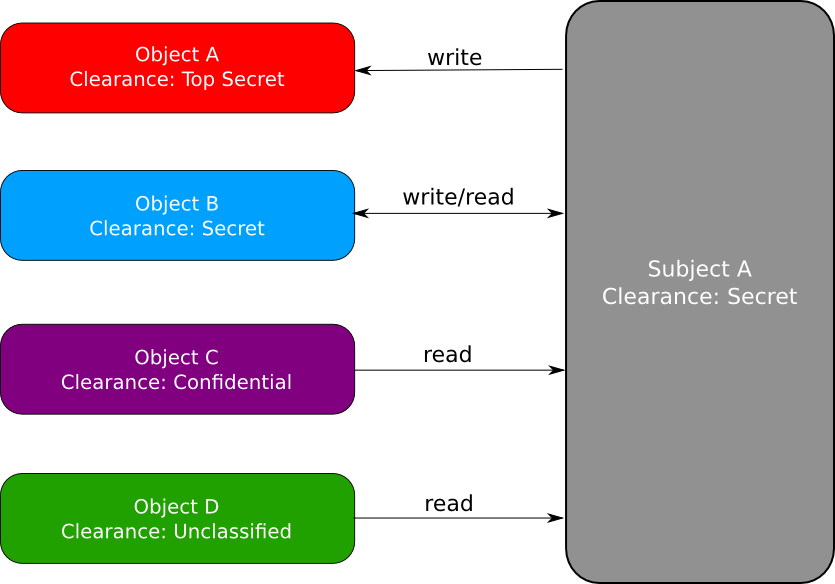
\includegraphics[width=1.0\linewidth]{gfx/chapter_2/blp_security_level_rules}
%\caption[BLP: Security Level rules]{BLP: Security Level read/write  %rules}\label{fig:blp_security_level_rules}
%\end{figure}

In addition to security level labels, as mentioned above, BLP can also be designed in combination with \emph{classification} labels to create a stronger restriction to object accesses.
Under the circumstances, the subject's classification labels should be a subset of the object's to be able gain the access permission.
If we call the subject's roles a set $R1$ and the object's $R2$, where

$$R1, R2 \in \{project manager, programmer, designer\}$$ 

The subject can gain access permission to R2 only if $R1 \subseteq R2$.
\autoref{fig:blp_security_level_roles_rules} shows the principles of handling request from a subject to the other objects regarding only to their security levels.

%\begin{figure}[bth]                                                                                                                                                  
%\myfloatalign
%\includegraphics[width=1.0\linewidth]{gfx/chapter_2/blp_security_level_roles_rules}
%\caption[BLP: A set of Security Level and Roles rules]{BLP: A set of Security %Level and Roles rules}\label{fig:blp_security_level_roles_rules}
%\end{figure}

Finally, a user can use \emph{Discretionary Access Control} (DAC) set the permission to an object.
\cite{centos:2008} cited that MLS access rules are always combined with \emph{conventional access permissions} (or file permission).
It means that if a user with security label \emph{Secret} uses DAC to block access to an object by the other uses, this also block access by by users with security level of \emph{Top Secret}.
Additionally, \cite{bancinco:2015} presented that
\begin{quote}
SELinux MLS policy rules are checked after DAC rules. A higher security clearance does not automatically give permission to arbitrarily browse a file system.
\end{quote}
Hence, \autoref{fig:blp_security_level_roles_rules} will be a mostly complete picture describing about BLP model after we put every components together.

In conclusion, MLS and BLP model in specification are suitable for many of real world organization models. It can isolate objects and protect them from multi-level accesses.

\begin{figure}[bth]
\myfloatalign
\subfloat[BLP: Security Level rules]
{\label{fig:blp_security_level_rules}
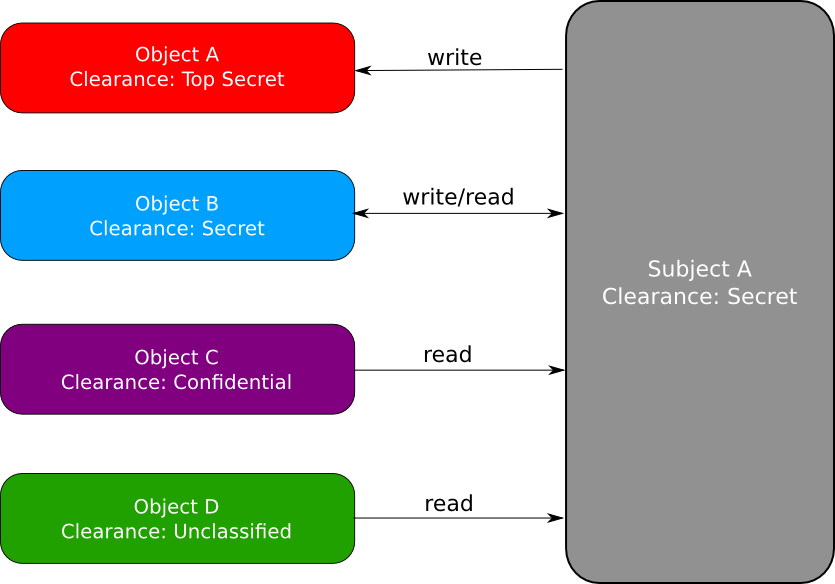
\includegraphics[width=.9\linewidth]{gfx/chapter_2/blp_security_level_rules}} \quad

\subfloat[BLP: A set of Security Level and Roles rules]
{\label{fig:blp_security_level_roles_rules}
\includegraphics[width=.9\linewidth]{gfx/chapter_2/blp_security_level_roles_rules}} \\

\subfloat[BLP: all components illustration]
{\label{fig:blp_example}
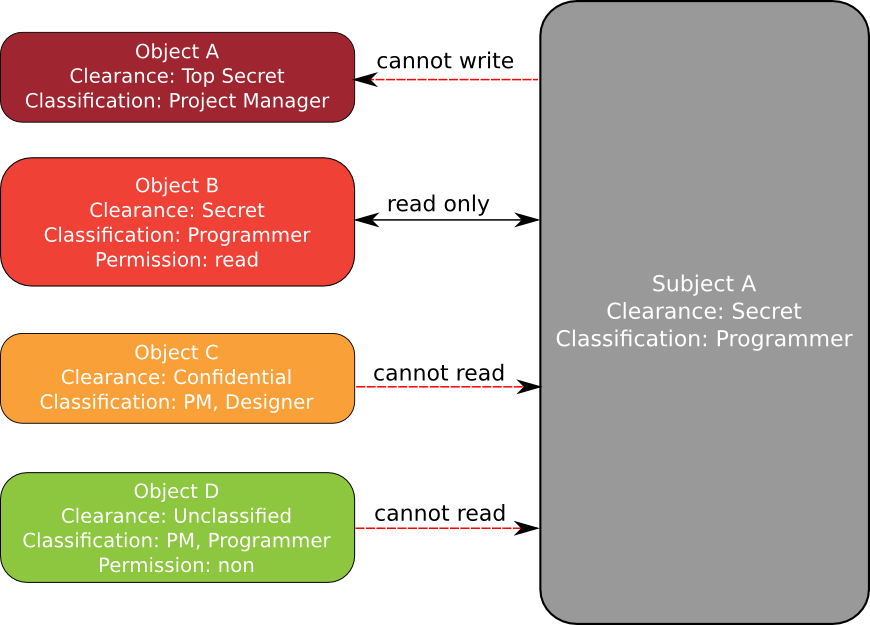
\includegraphics[width=.9\linewidth]{gfx/chapter_2/blp_example}} \\

\caption[BLP illustration]{Illustrate how BLP components relate to each others}\label{fig:blp_illustration}
\end{figure} 
 % Chapter 2
% Chapter 3

\chapter{HotPot Project} % Chapter title

\label{ch:hopot_project} % For referencing the chapter elsewhere, use \autoref{ch:hotpot_project}

%----------------------------------------------------------------------------------------

In \autoref{ch:background}, we learned that MLS is a very practical solution for multi-level access control.
It is very suitable to PMT because of the essence of PMT is sharing and collaborating among groups of people of different concerns and priorities.
As introduced in \autoref{ch:introduction:use_cases}, \myProject is a PMT implementing BLP model to ensure data security by forcing subjects to follow a set of predefined rules in order to gain access permission to objects.
In this chapter, I am going to explain in details the features of the project; how is it different from the other PMT; how does it approach the security demands.
By that way, we can understand precisely the goal of the project.

%----------------------------------------------------------------------------------------

\section{Concepts}
\label{ch:hopot_project:concepts}

By the time of writing this thesis, in the market, there are already plenty of PMTs with a huge number of features.
Some of popular names are Redmine, Workfront, FreshDesk, Genius Project etc...
Every tools has their own key features.
Go through their features list, we can see that most of features mainly focus on management and analyzing purposes.
They aim to provide customers most convenient tool with rich features and best user experience.
In term of security, most of the projects support SSL data encryption and apply vairous techniques to ensure data integrity.
Those traits can protect data on communicating progress, or keep it away from external exploits.
However, in order to protect internal assets from being accessed by authenticated users, most of them only support CAP which allow read/write permissions on an asset.
In fact, many of data leaking cases were reported done by authenticated but unauthorized users.
MLS perfectly matches into this scenario that it enforces all internal subjects to follow accessing policies, regardless of their priorities or the object's CAP.
In another word, every objects in the system will served exactly to groups of subjects who satisfy their admission requirements.
As the result, MLS is a eminently strong solution for lacking of MAC.
And that is also the main goal of \myProject that tries to implement BLP model to PMT.

\myProject is a PMT with essential features of managing projects.
At this stage, because of the purpose of this thesis, I only primarily focus on security practices of BLP in PMT.
And the management features are only enough to illustrate a general working PMT.

%------------------------------------------------

\subsection{Project Management Features}
\label{ch:hopot_project:concepts:pm_features} 

PMT is a platform in which users can plan their projects, create and track project tasks, project progress, team members' assignments etc...
In the market, many PMTs have outstanding user experience features.
They consist of performance analyzing and evaluation tool, both personally and organizationally.
Some even embed discussion forum, subversion control monitoring etc...
However in \myProject, I only focus on some essential features of a PMT in order to demonstrate the security features such as:

\begin{itemize}
\item Create and manage (edit, delete) accounts. There are two types of account: normal account and admin, we will go into details about these types in the next \autoref{ch:hopot_project:project_components:account}
\begin{itemize} 
\item Editting account's personal information (\eg full name, email, address, contact etc...). 
After logging in, users can update their own information.
\end{itemize}

\item Create and manage (edit, delete) projects.
\begin{itemize} 
\item Assigning members to projects. 
\item Setting project members' security labels (\eg \emph{security level}, \emph{roles}).
\end{itemize}
\item List all projects.
\item List project's members.

\item Create and manage (edit, delete) articles.
\begin{itemize} 
\item Creating directory.
\item Setting articles and directories' security labels (\eg \emph{security level}, \emph{roles}).
\end{itemize}
\item List project's articles: the result of the articles list will be different from users. Because each account will have different set of security labels.

\item Create and manage (edit, delete) tickets.
\begin{itemize} 
\item Tickets assigning.
\item Setting tickets' security labels (\eg \emph{security level}, \emph{roles}).
\end{itemize}
\item List project's tickets: this list is similar to articles list.

\item Create and manage (edit, delete) security components. \footnote{They are the core of the security policies}
\begin{itemize} 
\item Roles.
\item Security Levels.
\end{itemize}.

\end{itemize}

In the next \autoref{ch:hopot_project:concepts:security_features}, we will learn about the projects' \emph{security policies}.
It will help us to answer questions related to management features such as who can perform these functions? How security policies will affect their performance? etc...

%------------------------------------------------

\subsection{Security Features}
\label{ch:hopot_project:concepts:security_features}

This chapter focus on answering one big question \emph{How do we handle security?}
It will explain in details the \emph{security policies} of the project.
So that, We can understand how users can use this system? What rules they have to follow? And how the restriction can protect data by users with multi-level security?

Because of using MLS, first of all, we have to list all of the system's components, then categories them as either \emph{subject} or \emph{object}.
\emph{Subjects} are components which actively interact in the system \eg\ processes, users etc\dots
So, in our project, they are \emph{accounts} (or users, team members\dots) and another special type of account is \emph{administrators} (or admins for short).
On the other hand, \emph{objects} are passive components which are \emph{articles}, \emph{tickets}, and \emph{projects} in our case.
Rather than that, there are three elements that form the security policies for subjects and objects. They are \emph{security levels}, \emph{roles}, and \emph{read/write permissions}.
Every subjects and objects will have one security level label and at least one role. Besides that, all the objects will have one more CAP feature, so they can restrict the subjects' behaviors such as read or write.
In the system, there can be many projects developed at the same time.
Everyone, every subjects, can have different roles, and priorities in different projects.
Consequently, in order to ensure the system consistency, every subject in different projects will have different \emph{project profiles}.
Each profile consists of a different set of security labels, corresponding to the subject's characters in the project. %draw sth to illustrate this

In \myProject, there are main actions a subject can perform on an object: \emph{create, view, list, edit, delete}.
Some of them such as \emph{view, list} are considered as reading behavior, so that it requires \emph{read permission} on the objects for the subjects to perform.
In a different manner, \emph{create, edit and delete} require \emph{write permission} on the object for the subject to perform.
\marginpar{\emph{Edit} action need both read and write permission.}
However, considering about \emph{edit} action, we can see that in order for a subject to edit an object's contents, he must be able to read it first.
So \emph{edit} is a special case where it requires the object's both \emph{read} and \emph{write} permission.
\marginpar{\emph{Delete} action can only be done by the object's owner.}
Also \emph{delete} is also a sensitive action.
It is a \emph{write action}.
Yet, in term of data integrity, \emph{delete} action should only be executed by the object's owner \ie subject which created it.
Let's consider this scenario, a secret article should be created to report a fault of a team member to the managers.
If a manager with secrete label doesn't like that report, he can delete it.
Nevertheless, \emph{create} is also a distinctive action.
It also depends on other logical rules for the subject to perform.
For example, only team member can create articles and tickets of that project.
We will discuss about these kinds of special actions and logical rules in the upcoming \autoref{ch:hopot_project:project_components}.
According to BLP security policies explained in \autoref{ch:background:bell}, every subjects must own a set of security labels which full-fills the security policies again the target object's.
So in order to perform \emph{read action}, the subject's security level label should be higher or equals to the object's;
the subject's set of role labels must be a subset of the object's;
and the object must be readable \ie read permission is on.
On the other hand, the \emph{write action} requires the subject's security level label is lower or equals to the object's;
the subject's set of role labels must be a subset of the object's too;
and the object is set to writable mode.

% NOTE: add illustraion for the security decision.

On developing the project, I sometimes had to due with trade-off of strong security and convenient user experience.
Solving object's owner's security policies is one of the trade-off I had to make.
Let's consider a scenario.
A subject, with secret security label, creates an object \eg article with top secret label. 
After that, he needs to \emph{edit} the article, \eg add more information, but the security policies will prevent him from doing that because, as we explained above, he need to have the same security level with the artilce to \emph{edit} it.
This will be very inconvenient in case he has to edit the article many times.
On the contrary, if we allow the owner to read his objects regardless of their security level, it may be vulnerable to data leak.
Since, if a top secret subject decides to edit the object to add some sensitive data into it, the owner can still read them.
\marginpar{\emph{Trade-off}: a subject have all permissions on his own objects.}
However, thinking about the user experience and because the project aims to serve civil organizations of medium scale, I think it's better to let owners have all permissions on their own objects.
It also helps to solve the problem of \emph{delete} action that we discussed before.
\marginpar{\emph{Future plan}: logging system is needed to track all actions in the system, especially these kind of compromising actions that need the subjects' awareness.}
Because this is a compromise, so that we need a good practice to fix it.
It could be a system unrelated rule, that high security level subjects should not edit objects of lower security level subject, instead he should create a copy of it then add his additional information into the copy, unless he is only leaving comments on the object.

Furthermore, besides the BLP model policies, some logical rules are applied for some actions in the system.
These rules also have to follow the predefined security policies.
They are just like another layer of the access control to the actions.
For example, creating new subjects (accounts); managing relations among objects; creating new objects related to another objects etc\dots
Those logical rules will be discussed in the next \autoref{ch:hopot_project:project_components}.
%----------------------------------------------------------------------------------------

\section{Project Components and Use Cases}
\label{ch:hopot_project:project_components}

How we build the project? what we focus on? What security principle should the follow?

This chapter will explain about security behaviors of every components of the project.
We will learn about all the main features of the system, as well as how they are expected to behave against security policies.
Here, we also discuss about the logical polices that could be considered another layer of the access control.
Finally, we will explain most of the use cases of the project.
These use cases will be demonstrated illustratively later in \autoref{ch:result:user_guide}.

%------------------------------------------------

\subsection{Account and Administrator}
\label{ch:hopot_project:project_components:account}

Account is the main subject in our system.
There are two types of account: \emph{user account} and \emph{admin account}.
These two types of account have the same properties in database, however, due to their responsibilities ,they will have different behavior in the system.

A user account is the account type for most of everyone in the organization.
It consists of enough information of an employee \eg username, password, contact \dots
Below are lists of all actions the account can perform on other objects in the system. These actions will be explained in more detailed when will discuss about the other components in this chapter.

\afterpage{
%account
\begin{table}[!htbp]
\myfloatalign
\begin{tabularx}{\textwidth}{lX} 
\toprule
\tableheadline{Actions} & \tableheadline{Description}\\ 
\midrule
\emph{Create} & 
ONLY administrator can create new account.\\
\midrule
\emph{View} & 
Every account can view the other's details. 
This is because of the simplicity and convenience of the project.
In fact, there is no vital data in this area that can be exploited.\\
\midrule
\emph{Edit} & 
ONLY the \emph{account's owner} can update his own account's details. \\
\bottomrule
\midrule
\emph{Delete} & 
Administrator and the account owner can delete the account.\\
\end{tabularx}
\caption[Account's actions on account details.]{Account's actions on account details.}  
\label{tab:account_on_detail}
\end{table}

%project
\begin{table}[!htbp]
\myfloatalign
\begin{tabularx}{\textwidth}{lX} 
\toprule
\tableheadline{Actions} & \tableheadline{Description}\\ 
\midrule
\emph{Create} & 
Every account can create a new project. The creator account, then, will be set as the project's owner, and added to the project as a project member.\\
\midrule
\emph{View} & 
Every account can view the project information. 
However, the visitor cannot see the list of articles and tickets of the project.\\
\midrule
\emph{Edit} & 
ONLY the \emph{project owner} can update the project's information. \\
\midrule
\emph{Add member} & 
ONLY the \emph{project owner} can add the other accounts to his project. \footnote{Every accounts added to a project will have one \emph{project profile} where store all of the account's security labels in that project} \\
\midrule
\emph{Edit member permission} & 
ONLY administrators can perform this action. \\
\midrule
\emph{Delete} & 
ONLY the \emph{project's owner} can delete the project. \\
\bottomrule
\end{tabularx}
\caption[Account's actions on projects.]{Account's actions on projects.}  
\label{tab:account_on_project}
\end{table}

%article
\begin{table}[!htbp]
\myfloatalign
\begin{tabularx}{\textwidth}{lX} 
\toprule
\tableheadline{Actions} & \tableheadline{Description}\\ 
\midrule
\emph{Create} & 
Every project member can create new articles of that project. The creator account, then, will be set as the article's owner. This action must follow the security policies in \autoref{ch:hopot_project:concepts:security_features}.\\
\midrule
\emph{List} & 
Every project member can see the list of project's articles.
The list only shows articles related to the member's security labels, that follow the security policies in \autoref{ch:hopot_project:concepts:security_features}.\\
\midrule
\emph{View} & 
Every project member can view the project's articles.
This action must follow the security policies in \autoref{ch:hopot_project:concepts:security_features}.\\
\midrule
\emph{Edit} & 
Every project member can edit the project's articles. 
This action must follow the security policies in \autoref{ch:hopot_project:concepts:security_features}.\\
\midrule
\emph{Add article to directory} & 
Every project member can add articles to a the project's article directory 
\footnote{\emph{Article} and \emph{directory} relation will be discuss in \autoref{ch:hopot_project:article}}.
Adding an article to a directory is considered as editing the directory so that this action must follow the security policies in \autoref{ch:hopot_project:concepts:security_features} against on directory.\\
\midrule
\emph{Delete} & 
ONLY the \emph{article's owner} can delete it. \\
\bottomrule
\end{tabularx}
\caption[Account's actions on articles.]{Account's actions on articles.}  
\label{tab:account_on_article}
\end{table}

%ticket
\begin{table}[!htbp]
\myfloatalign
\begin{tabularx}{\textwidth}{lX} 
\toprule
\tableheadline{Actions} & \tableheadline{Description}\\ 
\midrule
\emph{Create} & 
Every project member can create new tickets of that project. The creator account, then, will be set as the ticket's owner. This action must follow the security policies in \autoref{ch:hopot_project:concepts:security_features}.\\
\midrule
\emph{List} & 
Every project member can see the list of project's tickets.
The list only shows tickets related to the member's security labels, that follow the security policies in \autoref{ch:hopot_project:concepts:security_features}.\\
\midrule
\emph{View} & 
Every project member can view the project's tickets.
This action must follow the security policies in \autoref{ch:hopot_project:concepts:security_features}.\\
\midrule
\emph{Edit} & 
Every project member can edit the project's tickets. 
This action must follow the security policies in \autoref{ch:hopot_project:concepts:security_features}.\\
\midrule
\emph{Assign ticket} & 
This action is similar to \emph{edit} action.\\
\midrule
\emph{Delete} & 
ONLY the \emph{ticket's owner} can delete it. \\
\bottomrule

\end{tabularx}
\caption[Account's actions on tickets.]{Account's actions on tickets.}  
\label{tab:account_on_ticket}
\end{table}
}

Besides that, there are some actions on security related components like \emph{security labels}, \emph{role} that can only be performed by \emph{administrator accounts}. Administrators have all permissions on these special components. Besides that, they are the only ones who can edit other accounts' security labels.
\cleardoublepage %fix the tables' appearance problems

%------------------------------------------------

\subsection{Project}
\label{ch:hopot_project:project_components:project}

Project is not actually neither subject nor object of the system.
In the manner of management, it's just a grouping element to group related objects \eg accounts, articles and tickets.

According to \autoref{tab:account_on_detail}, all accounts can create new project.
Then, the project's owner can add other accounts to the project as team members.
Each of the team members will have one \emph{project profile} which store all needed information for the system to apply the security policies on the member's actions \eg \emph{security level}, roles.
By that design, every accounts will have different priorities in different projects, which provide a flexible management in the organization.
Moreover, only the owner can edit and delete the project.

Each projects has its own lists of articles and tickets.
Only the project's team members can access them \eg create, edit, list, view delete.

%------------------------------------------------

\subsection{Security Level (Clearance)}
\label{ch:hopot_project:project_components:security_level}

\emph{Security Level} is one of the security components.
It represent the \emph{clearance} property of objects and subjects.
Only an administrator can access to perfom actions on this component.
The \emph{security level label} has a \emph{level} property to indicate its priority.
The higher number the level, the more important the owner is.
For example, \emph{Secret} label has the \emph{level} value of 3, and \emph{Top Secret} has the value of 4.
The name of the security level label as well as its priority level can completely be decided by the system's administrators.
In another word, the administrators can modify the system's appearance as his will. 
The security level label will relate to an account via his project profiles. Every account's project profiles will have a different one.

%------------------------------------------------

\subsection{Role (Classification)}
\label{ch:hopot_project:role}

Like \emph {Security Level}, \emph{Role} is also a security component of the system.
It indicate subjects, objects' categories \ie \emph{classification}.
As we discussed in previous \autoref{ch:background:bell}, one subject or object can have various role labels.
And a subject's roles have to be a subset of the object's in order for the subject to access it.
Similar to \emph{Security Level}, \emph{Roles} also relate to an account via hist project profiles. 
In another word, one subject may have different roles in different project.
Indeed, it's a great common scenario in organizations.


%------------------------------------------------

\subsection{Article and Directory}
\label{ch:hopot_project:article}

\emph{Article} is one of two main objects of the system.
Article could be any kinds of document.
It could be a report, technical notes, project related documentation etc\dots
Every article belongs to a particular project.
Any team member in the project can create new articles.
While every other team members have to full-fills the security policies described in \autoref{ch:background:bell} in order to access an article, the article's owner has all permission on it.
And, only the owner can delete his articles.

In some cases, many articles, which relate to each other and share similar security policies, should be grouped together.
It helps us to manage articles better, and provides a flexible hierachy for sharing articles.
In that manner, \emph{Directory} is designed to deliver that feature.
In fact, \emph{directory} is an \emph{article}.
It means that it has all article's properties, and follows all article's security policies, except that a directory can have the other articles as its children.
The children articles created inside a directory should have equal or higher \emph{security level} than the directory.
So that, team members can \emph{create} new article inside the directory without getting restricted by security polices.
Rather than that, the children should have a set of roles which is a subset of the directory's roles.
It will generate a common sense for team members when they want to find some articles inside a directory, they can check the directory's roles to know the children's categories.
Finally, because \emph{directory} is an \emph{article}, so it also have read and write permission on it.

%------------------------------------------------

\subsection{Ticket}
\label{ch:hopot_project:ticket}

Just like \emph{Article}, \emph{Ticket} is also a kind of subject of the system.
It also need to follow security policies defined in \autoref{ch:background:bell}, and it belongs to projects too.
Every tickets will have an owner (or creator) and an assignee property.
Assigning an assignee to a ticket is also considered as an \emph{edit action}, so that the subject who performs it also need full-fills the edit policies.
Moreover, the assignee's security policies should satisfy the ticket's.
 % Chapter 3
% Chapter 4

\chapter{Implementation} % Chapter title

\label{ch:implementation} 
% For referencing the chapter elsewhere, use \autoref{ch:name} 

%---------------------------------------------------------------------------------------- 

From previous chapters, we studied about concepts of a MLS system, as well as logical security policies in the manner of PM.
They together form a list of essential features of a MLS-implemented PMT.
In another world, so far, we had a blueprint of a MLS PMT. 
My \myProject project is built upon this blueprint.
The project's purpose is to evaluate the possibility of my theory and to answer these questions.

\begin{enumerate}
\item How much effort is needed to build a MLS system? 
\item How practically they are used in PM?
\item And how much does it affect to user experience?
\end{enumerate}

In this chapter, we are going to cover the implementation of the project.
It consists of the project's agenda, technical requirements, the program architecture, its data models and their corresponding database schema, relations among data models, etc\dots

%----------------------------------------------------------------------------------------

\section{Project agenda}
\label{ch:implementation:project_agenda}

\autoref{fig:hotpot_gantchart} is my very first Gant chart of developing time of my project.
Later, although there has been couples of small changes in the time line, however, basically the project finished as scheduled.

\begin{figure}[bth]                                                                                                                                                  
\myfloatalign
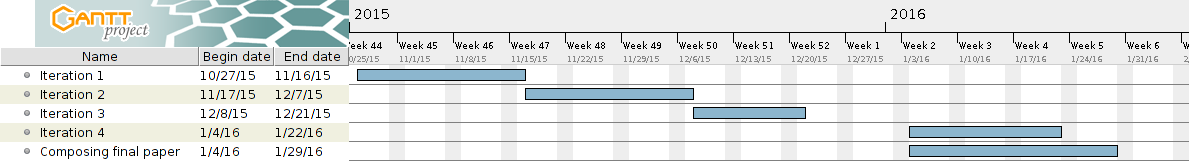
\includegraphics[width=1.0\linewidth]{gfx/chapter_4/hotpot_gantchart}
\caption[HotPot Gant chart]{BLP: HotPot Gant Chart}
\label{fig:hotpot_gantchart}
\end{figure}

The project has four iterations, each of which is three weeks long.

\begin{description}
\item[First iteration]
From 27/10/2015 to 16/11/2015
\begin{itemize}
\item Setup environment. 
\item Create initial DB schema. 
\item Create \emph{account} model with associated details. 
\item Create \emph{project} model. 
\item Add/remove accounts into/from projects. 
\item Create roles, security level. 
\item Assign account to many roles, and one security level.
\end{itemize}

\item[Second iteration]
From 17/11/2015 to 7/12/2015
\begin{itemize}
\item Create \emph{article} model.
\item Assigning security level and role to articles. 
\item Handling user login.
\item List projects related to current logged in account.
\item List articles related to current logged in account.
\end{itemize}

\item[Third iteration]
From 8/12/2015 to 29/12/2015
\begin{itemize}
\item Setup security logic on article actions (\eg create, view, list, edit, delete\dots). 
\item Create \emph{ticket} model. 
\item Apply security logic to ticket actions.
\end{itemize}

\item[Fourth iteration]
From 4/1/2016 to 31/1/2016
\begin{itemize}
\item Fix and update new security logics on \emph{objects' actions}.
\item Implement \emph{directory} structure for managing articles.
\item Apply graphical design.
\item Writing thesis documents and reports.
\end{itemize}
\end{description}
 
Every iterations has one or two days different from the planed schedule, however, in general, the programming part was completed as scheduled.

%----------------------------------------------------------------------------------------

\section{Technical information}
\label{ch:implementation:technical_information} 

In this section, I am going to introduce about the technologies used in this project, as well as the reason why I chose them at the first place.
The list below are technologies used in the project's developing environment:

\begin{description}
\item[OS] \emph{Ubuntu 14.04}.
It's a free, open source and widely used Linux distro developed by \emph{Canonical Ltd}.
It is easy to use, convenient, and strongly supported by a huge community.
I also used {Vagrant} (\emph{HashiCorp}) and \emph{VirtualBox} (\emph{Oracle}) for virtual environment.
\item[Programming language] \emph{Javascript - Nodejs}.
It's a very dynamic programming language which has an increasing number of developers.
This is my second project using Javascript on back-end, and it's the first project I work with back-end Javascript - Nodejs on my own. It's only for learning purpose, and indeed, I learned many things from this project.
\item[Framework and libraries] \emph{Expressjs, Sequelizejs}.
Expressjs may be the most popular web framework for Nodejs.
It has apparent documentation and a strong community.
Sequelizejs, on the other hand, is a famous and stable DAO library for Nodejs.
\item[Database] \emph{PostgreSQL} is my best choice of SQL Database.
It supports various data types and useful features.
Moreover, it has many libraries to be used in numerous programming language.
\item[Subversion control] \emph{Git} as the tool and \emph{GitHub} as the repository.
\item[Text Editors] \emph{Vim} for coding and \latex for composing thesis papers. And, as the \latex template, I use \emph{Classicthesis Typographic Thesis} of \emph{Andr\'{e} Miede}.

\end{description}

In fact, after finishing developing, I deployed a sample of my project on a cloud machine.
Most of the technical requirements are the same except that I used \emph{CentOS} (\emph{RedHat Inc} instead of Ubuntu for testing purpose and I can confirm that it works on \emph{CentOS} as well.
I can find every things needed on CentOS just like on Ubuntu.

%----------------------------------------------------------------------------------------

\section{Models}
\label{ch:implementation:models}

This section is a summary of my project's design.
I utilized MVC design model in this project.
All the logical controls will go to \emph{controllers}, which handle all the security policies as previously described in \autoref{ch:background:bell}.
So that, in this thesis document, I only focus explaining about the project's models and their relationship so that we can understand about the system's architecture.

In this section, I am going to list all the data models of the system.
We will learn about their properties, relations which will be illustrated as database diagrams.
\autoref{fig:er_diagram} is an \emph{ER diagram} including all data tables and their mutual relations in the system.

\begin{figure}[bth]                                                                                                                                                  
\myfloatalign
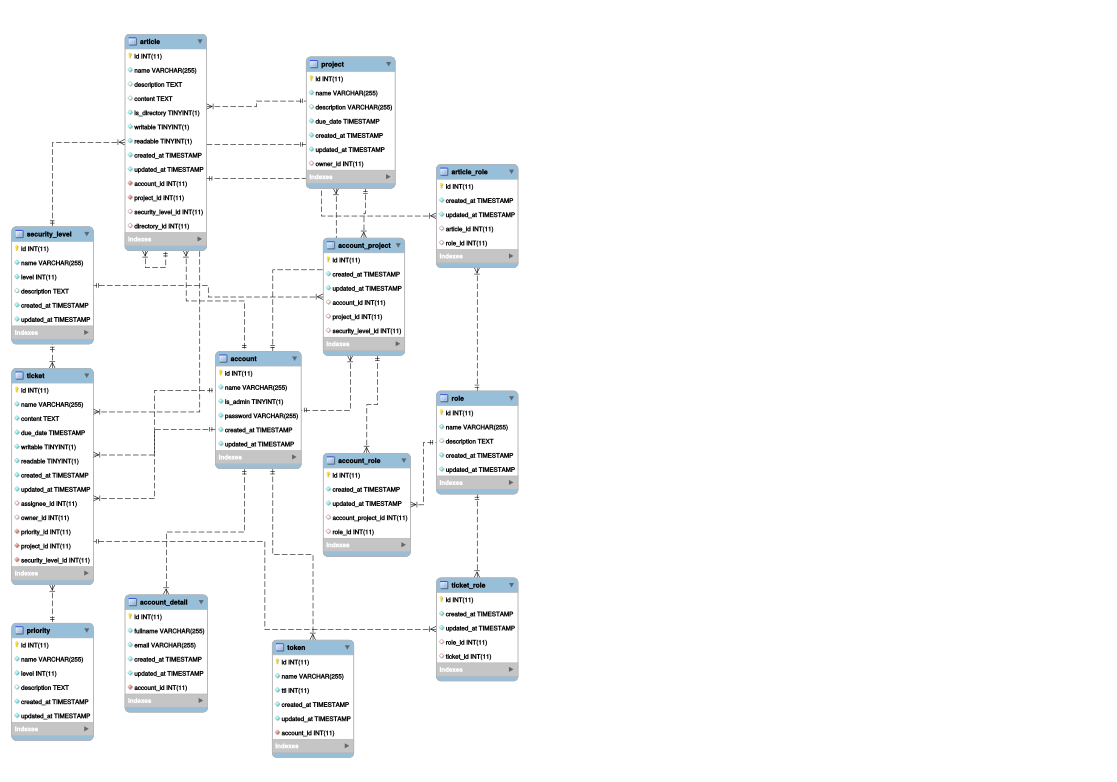
\includegraphics[width=1.0\linewidth]{gfx/chapter_4/er_diagram}
\caption[Entity Relation Diagram]{Entity Relation Diagram}
\label{fig:er_diagram}
\end{figure}
\clearpage

%------------------------------------------------

\subsection{Account}

\emph{Account} model corresponds to \emph{account subject} in the system.
It only consists of authentication and identity information of an account.
\autoref{tab:account_model_properties} explains all the properties of \emph{account} model, while \autoref{tab:account_model_relations} shows the relations between \emph{account} and the others in the system.

\begin{table}[!htbp]
\myfloatalign
\begin{tabularx}{\textwidth}{lXX} 
\toprule
\tableheadline{Property} & \tableheadline{Type} & \tableheadline{Description}\\ 
\midrule
\emph{name} &
string, not null, unique & 
The account's user name for logging in.\\
\midrule
\emph{password} & 
string, not null &
The account's password.\\
\midrule
\emph{password\_confirm} & 
string, not null &
This is a virtual field, which means it doesn't exist in the database table, and used for confirming password on account creation. \\
\midrule
\emph{is\_admin} & 
boolean, not null, default value: false &
Indicate whether an account is an administrator or not.\\
\bottomrule
\end{tabularx}
\caption[Account model properties.]{\emph{account} model properties.}  
\label{tab:account_model_properties}
\end{table}

\begin{table}[!htbp]
\myfloatalign
\begin{tabularx}{\textwidth}{llX} 
\toprule
\tableheadline{Model} & \tableheadline{Relation} & \tableheadline{Description}\\ 
\midrule
\emph{token} &
1:1 & 
Every account will have one new token for every logging in.\\
\midrule
\emph{account\_detail} & 
1:1 &
The account's detail information \eg full name, email, phone \dots \\
\midrule
\emph{project} & 
many:many &
An account may join many projects. 
This m:m relationship is defined through \emph{account\_project} model \ie relation table.\\
\midrule
\emph{account\_project} & 
1:many &
This is the relation model between \emph{account} and \emph{project} models to define the m:m relation.
In another word, it defines an account's \emph{project profiles}.
More about \emph{project profile} is explained in \autoref{ch:implementation:models:account_project} \\
\midrule
\emph{project} & 
1:many &
This relation is used for defining the account's \emph{owned projects}.
So once an account create a project, he will become that project's owner.\\
\midrule
\emph{article} & 
1:many &
This relation is used for defining the account's \emph{owned articles}.\\
\midrule
\emph{ticket} & 
1:many &
This relation is used for defining the account's \emph{owned tickets}.\\
\midrule
\emph{ticket} & 
1:many &
This relation is used for defining the account's \emph{assigned articles}.\\
\bottomrule
\end{tabularx}
\caption[Account model relations.]{Relations between \emph{account} and other models}  
\label{tab:account_model_relations}
\end{table}
\clearpage %to fix the float table problem.

%------------------------------------------------

\subsection{Account Detail}

This data model represents an account's detailed information. Its properties is listed in \autoref{tab:account_detail_model_properties}, and its relations to other models are explained in \autoref{tab:account_detail_model_relations}.

\begin{table}[!htbp]
\myfloatalign
\begin{tabularx}{\textwidth}{lXX} 
\toprule
\tableheadline{Property} & \tableheadline{Type} & \tableheadline{Description}\\ 
\midrule
\emph{fullname} &
string, not null, length between 8 and 128 & 
The account's fullname.\\
\midrule
\emph{email} & 
string, not null, unique &
The account's email address.\\
\bottomrule
\end{tabularx}
\caption[Account Detail model properties.]{\emph{account\_detail} model properties.}  
\label{tab:account_detail_model_properties}
\end{table}

\begin{table}[!htbp]
\myfloatalign
\begin{tabularx}{\textwidth}{llX} 
\toprule
\tableheadline{Model} & \tableheadline{Relation} & \tableheadline{Description}\\ 
\midrule
\emph{account} & 
1:1 &
One \emph{account\_detail} belongs to one \emph{account} and vice versa. \\
\bottomrule
\end{tabularx}
\caption[Account Detail model relations.]{Relations between \emph{account\_detail} and other models}  
\label{tab:account_detail_model_relations}
\end{table}
\clearpage %to fix the float table problem.

%------------------------------------------------

\subsection{Project}

This model contains all the information of a project. Its details are described in two table \autoref{tab:project_model_properties} and \autoref{tab:project_model_relations}

\begin{table}[!htbp]
\myfloatalign
\begin{tabularx}{\textwidth}{lXX} 
\toprule
\tableheadline{Property} & \tableheadline{Type} & \tableheadline{Description}\\ 
\midrule
\emph{name} &
string, not null, unique & 
The \emph{project}'s name.\\
\midrule
\emph{description} & 
string, allow null, length between 8 and 128  &
The \emph{project}'s description.\\
\midrule
\emph{due\_date} & 
date, allow null  &
The \emph{project}'s deadline.\\
\bottomrule
\end{tabularx}
\caption[Project model properties.]{\emph{project} model properties.}  
\label{tab:project_model_properties}
\end{table}

\begin{table}[!htbp]
\myfloatalign
\begin{tabularx}{\textwidth}{llX} 
\toprule
\tableheadline{Model} & \tableheadline{Relation} & \tableheadline{Description}\\ 
\midrule
\emph{account} & 
many:many &
A \emph{project} may have many \emph{members}. 
This m:m relationship is defined through \emph{account\_project} model. \\
\midrule
\emph{account} & 
many:1 &
This relation is used for defining the \emph{project}'s \emph{owner}.\\
\midrule
\emph{article} & 
1:many &
This relation is used for defining the \emph{project}'s \emph{articles}.\\
\midrule
\emph{ticket} & 
1:many &
This relation is used for defining the \emph{project}'s \emph{tickets}.\\
\bottomrule
\end{tabularx}
\caption[Project model relations.]{Relations between \emph{project} and other models}  
\label{tab:project_model_relations}
\end{table}
\clearpage %to fix the float table problem.

%------------------------------------------------

\subsection{Account Project (Project Profile)}
\label{ch:implementation:models:account_project}

\emph{account\_project} is a special model.
It is the relation table used to define the \emph{m:m} relation between \emph{account} and \emph{project} model.
Rather than that, it also contains all the information relating to a project of an account \eg his \emph{security level}, \emph{roles}.
In another word, this model contains all the security information of an account in a project, that we can use to authorize the account's access requests to the project's objects later.
In that manner, we also call this model a \emph{project\_profile} model.
Because this is only a relation model, there is no properties in it.
Its relations to other models are defined in \autoref{tab:account_project_model_relations}

\begin{table}[!htbp]
\myfloatalign
\begin{tabularx}{\textwidth}{llX} 
\toprule
\tableheadline{Model} & \tableheadline{Relation} & \tableheadline{Description}\\ 
\midrule
\emph{account} & 
many:many &
A project may have many \emph{members}. 
This m:m relationship is defined through \emph{account\_project} model. \\
\midrule
\emph{account} & 
1:1 &
This relation is used for defining the \emph{profile}'s \emph{account} (aka owner).\\
\midrule
\emph{project} & 
1:1 &
This relation is used for defining the \emph{profile}'s \emph{project}.\\
\midrule
\emph{security\_level} & 
1:1 &
This relation is used for defining the \emph{profile}'s \emph{security\_level}.\\
\midrule
\emph{role} & 
many:many &
This relation is used for defining the \emph{profile}'s \emph{roles}.
One profile may have many roles.\\
\bottomrule
\end{tabularx}
\caption[Account Project model relations.]{Relations between \emph{account\_project} and other models}  
\label{tab:account_project_model_relations}
\end{table}
\clearpage %to fix the float table problem.

%------------------------------------------------
\subsection{Security Level}

\emph{security\_level} model defines essential information of a security level label. Its details are described in two table \autoref{tab:security_model_properties} and \autoref{tab:security_model_relations}

\begin{table}[!htbp]
\myfloatalign
\begin{tabularx}{\textwidth}{lXX} 
\toprule
\tableheadline{Property} & \tableheadline{Type} & \tableheadline{Description}\\ 
\midrule
\emph{name} &
string, not null, unique & 
The \emph{security level}'s name.\\
\midrule
\emph{description} & 
string, allow null &
The \emph{security level}'s description.\\
\midrule
\emph{level} & 
integer, not null, unique &
The \emph{security level}'s level.
The higher value, the more important it is.\\
\bottomrule
\end{tabularx}
\caption[Security Level model properties.]{\emph{security\_level} model properties.}  
\label{tab:security_model_properties}
\end{table}

\begin{table}[!htbp]
\myfloatalign
\begin{tabularx}{\textwidth}{llX} 
\toprule
\tableheadline{Model} & \tableheadline{Relation} & \tableheadline{Description}\\ 
\midrule
\emph{account\_project} & 
1:many &
A \emph{security level} label may be used to tag on many \emph{accounts}.\\
\midrule
\emph{article} & 
1:many &
A \emph{security level} label may be used to tag on many \emph{articles}.\\
\midrule
\emph{ticket} & 
1:many &
A \emph{security level} label may be used to tag on many \emph{articles}.\\
\bottomrule
\end{tabularx}
\caption[Security Level model relations.]{Relations between \emph{security\_level} and other models}  
\label{tab:security_model_relations}
\end{table}
\clearpage %to fix the float table problem.

%------------------------------------------------

\subsection{Role}

\emph{role} model defines essential information of a role label.
Its details are described in two table \autoref{tab:role_model_properties} and \autoref{tab:role_model_relations}

\begin{table}[!htbp]
\myfloatalign
\begin{tabularx}{\textwidth}{lXX} 
\toprule
\tableheadline{Property} & \tableheadline{Type} & \tableheadline{Description}\\ 
\midrule
\emph{name} &
string, not null, unique & 
The \emph{role}'s name.\\
\midrule
\emph{description} & 
string, allow null &
The \emph{role}'s description.\\
\bottomrule
\end{tabularx}
\caption[Role model properties.]{\emph{role} model properties.}  
\label{tab:role_model_properties}
\end{table}

\begin{table}[!htbp]
\myfloatalign
\begin{tabularx}{\textwidth}{llX} 
\toprule
\tableheadline{Model} & \tableheadline{Relation} & \tableheadline{Description}\\ 
\midrule
\emph{account\_project} & 
many:many &
One or many \emph{role} labels may be used to tag on many \emph{profiles}.
This relation is defined through \emph{account\_role} model.\\
\midrule
\emph{article} & 
many:many &
One or many \emph{role} labels may be used to tag on many \emph{articles}.
This relation is defined through \emph{article\_role} model.\\
\midrule
\emph{ticket} & 
many:many &
One or many \emph{role} labels may be used to tag on many \emph{articles}.
This relation is defined through \emph{ticket\_role} model.\\
\bottomrule
\end{tabularx}
\caption[Role model relations.]{Relations between \emph{role} and other models}  
\label{tab:role_model_relations}
\end{table}
\clearpage %to fix the float table problem.

%------------------------------------------------

\subsection{Article}

\emph{article} model defines essential information of an article.
Its details are described in two table \autoref{tab:article_model_properties} and \autoref{tab:article_model_relations}

\begin{table}[!htbp]
\myfloatalign
\begin{tabularx}{\textwidth}{lXX} 
\toprule
\tableheadline{Property} & \tableheadline{Type} & \tableheadline{Description}\\ 
\midrule
\emph{name} &
string, not null & 
The \emph{article}'s name.\\
\midrule
\emph{description} & 
string, allow null &
The \emph{article}'s description.\\
\midrule
\emph{content} & 
string, allow null &
The \emph{article}'s content.\\
\midrule
\emph{is\_directory} & 
boolean, not null, default false &
Indicate whether this article is a directory or not.\\
\midrule
\emph{writable} & 
boolean, not null, default false &
Indicate whether this article is writable or not.\\
\midrule
\emph{readable} & 
boolean, not null, default false &
Indicate whether this article is readable or not.\\
\bottomrule
\end{tabularx}
\caption[Article model properties.]{\emph{article} model properties.}  
\label{tab:article_model_properties}
\end{table}

\begin{table}[!htbp]
\myfloatalign
\begin{tabularx}{\textwidth}{llX} 
\toprule
\tableheadline{Model} & \tableheadline{Relation} & \tableheadline{Description}\\ 
\midrule
\emph{account} & 
many:1 &
This relation is used for defining the \emph{article}'s \emph{owner}.\\
\midrule
\emph{project} & 
many:1 &
This relation is used for defining in which \emph{project} the \emph{article} belongs to.\\
\midrule
\emph{roles} & 
many:many &
An \emph{article} may have one or many \emph{role} labels.
This relation is defined through \emph{article\_role} model.\\
\midrule
\emph{security\_level} & 
many:1 &
This relation is used for defining the \emph{article}'s \emph{security level} label.\\
\midrule
\emph{article} & 
1:many &
If this \emph{article} is a directory, this relation defines \emph{articles} belong to it.\\
\midrule
\emph{article} & 
many:1 &
This relation is used for defining the \emph{article}'s \emph{directory} if available.\\
\bottomrule
\end{tabularx}
\caption[Article model relations.]{Relations between \emph{article} and other models}  
\label{tab:article_model_relations}
\end{table}
\clearpage %to fix the float table problem.

%------------------------------------------------

\subsection{Priority}

\emph{priority} is a property of \emph{ticket} model.
So, in order to provide a scalable system, I added this table for users to insert the suitable priorities for their system.
This model defines essential information of a priority.
Its details are described in two table \autoref{tab:priority_model_properties} and \autoref{tab:priority_model_relations}

\begin{table}[!htbp]
\myfloatalign
\begin{tabularx}{\textwidth}{lXX} 
\toprule
\tableheadline{Property} & \tableheadline{Type} & \tableheadline{Description}\\ 
\midrule
\emph{name} &
string, not null, unique & 
The \emph{priority}'s name.\\
\midrule
\emph{description} & 
string, allow null &
The \emph{priority}'s description.\\
\midrule
\emph{level} & 
integer, not null, unique &
The \emph{priority}'s level.
The higher level, the higher priority.\\
\bottomrule
\end{tabularx}
\caption[Priority model properties.]{\emph{priority} model properties.}  
\label{tab:priority_model_properties}
\end{table}

\begin{table}[!htbp]
\myfloatalign
\begin{tabularx}{\textwidth}{llX} 
\toprule
\tableheadline{Model} & \tableheadline{Relation} & \tableheadline{Description}\\ 
\midrule
\emph{ticket} & 
1:many &
This relation is used for defining \emph{tickets} with the \emph{priority}.\\
\bottomrule
\end{tabularx}
\caption[Priority model relations.]{Relations between \emph{priority} and other models}  
\label{tab:priority_model_relations}
\end{table}
\clearpage %to fix the float table problem.

%------------------------------------------------

\subsection{Ticket}

\emph{ticket} model defines essential information of an ticket.
Its details are described in two table \autoref{tab:ticket_model_properties} and \autoref{tab:ticket_model_relations}

\begin{table}[!htbp]
\myfloatalign
\begin{tabularx}{\textwidth}{lXX} 
\toprule
\tableheadline{Property} & \tableheadline{Type} & \tableheadline{Description}\\ 
\midrule
\emph{name} &
string, not null & 
The \emph{ticket}'s name.\\
\midrule
\emph{content} & 
string, not null &
The \emph{ticket}'s content.\\
\midrule
\emph{due\_date} & 
date, allow null &
The \emph{ticket}'s deadline.\\
\midrule
\emph{writable} & 
boolean, not null, default false &
Indicate whether this ticket is writable or not.\\
\midrule
\emph{readable} & 
boolean, not null, default false &
Indicate whether this ticket is readable or not.\\
\bottomrule
\end{tabularx}
\caption[Ticket model properties.]{\emph{ticket} model properties.}  
\label{tab:ticket_model_properties}
\end{table}

\begin{table}[!htbp]
\myfloatalign
\begin{tabularx}{\textwidth}{llX} 
\toprule
\tableheadline{Model} & \tableheadline{Relation} & \tableheadline{Description}\\ 
\midrule
\emph{account} & 
many:1 &
This relation is used for defining the \emph{ticket}'s \emph{owner}.\\
\midrule
\emph{account} & 
many:1 &
This relation is used for defining the \emph{ticket}'s \emph{assignee}.\\
\midrule
\emph{project} & 
many:1 &
This relation is used for defining in which \emph{project} the \emph{ticket} belongs to.\\
\midrule
\emph{roles} & 
many:many &
An \emph{ticket} may have one or many \emph{role} labels.
This relation is defined through \emph{ticket\_role} model.\\
\midrule
\emph{security\_level} & 
many:1 &
This relation is used for defining the \emph{ticket}'s \emph{security level} label.\\
\midrule
\emph{priority} & 
1:many &
This relation is used for defining the \emph{ticket}'s \emph{priority} label.\\
\bottomrule
\end{tabularx}
\caption[Ticket model relations.]{Relations between \emph{ticket} and other models}  
\label{tab:ticket_model_relations}
\end{table}
\clearpage %to fix the float table problem.

%----------------------------------------------------------------------------------------
 % Chapter 4
% Chapter 5

\chapter{Project Outcome} % Chapter title

\label{ch:outcome} 
% For referencing the chapter elsewhere, use \autoref{ch:outcome} 

%----------------------------------------------------------------------------------------

The project ended up with a web-based project management system.
The system consists of basic managing features which cover most common scenarios in PMT.
Besides that, the system also follows a set of MLS policies described in \autoref{ch:background:bell}.
This chapter includes an installation guide to setup the project from fresh; 
the system's user guide which describes its features and their usage demonstrations.
And at the end, I will discuss about my learning from the project's developing progress.

%----------------------------------------------------------------------------------------

\section{Installation Guide}
\label{ch:result:installation_guide}

\autoref{ch:implementation:technical_information} listed the technical requirements for this project.
In this guide, we will learn about the project's setup from scratch, step by step.

Assume that you already have a machine running CentOS 7 with these packages have already been installed: \emph{git, postgresql, nodejs with npm}.
I am using \emph{Digital Ocean} as VPS provider.
I create a \emph{Digital Ocean's droplet} with this specification: \emph{512MB Ram 20GB SSD Disk CentOS 7.1 x64}.
A postgresql database should be created and named as \emph{hotpot} whose owner is \emph{hotpot} and the password at your own choice.

First of all we need to clone the project's source code from GitHub using the command.
\begin{lstlisting}[breaklines=false,frame=lt]
$ git clone git@github.com:khangpn/hotpot.git
\end{lstlisting}

Next, we need to install all the project's dependencies by going into the project's root directory and execute \emph{npm} install command
\begin{lstlisting}[breaklines=false,frame=lt]
$/hotpot/ npm install
\end{lstlisting}
This command may take a while to install all required packages.

After checking the database accessibility, we need to configure its connection in \emph{config\/database.js}. 
Open that file by your favorite text editor, my choice is \emph{vim}. 
\begin{lstlisting}[breaklines=false,frame=lt]
$/hotpot/ vim config/database.js
\end{lstlisting}

Below is an example of the database configuration, if you named the database, its user and password are \emph{hotpot} and the database is running on local machine, then your configuration file should be similar to this.
\begin{lstlisting}[breaklines=false,frame=lt]
var settings = {                                                                                                                                                     
  development: { 
    database : "hotpot",
    username : "hotpot",
    password : "hotpot",
    options  : { 
      dialect : "postgresql",
      host     : "127.0.0.1"   
    }
  },
  production: { 
    database : "hotpot",
    username : "hotpot",
    password : "hotpot",
    options  : { 
      dialect : "postgresql",  
      host     : "127.0.0.1"   
    }
  }
};
  
module.exports = settings;
\end{lstlisting}

Next, lets open file \emph{setup} and change its \emph{NODE\_ENV} to \emph{development} or \emph{production} depending on your purpose.
\emph{Development} environemnt will print out the system's logs on our server and return errors' full stack trace to client, while  \emph{production} will omit it.
\begin{lstlisting}[breaklines=false,frame=lt]
// file hotpot/setup
NODE_ENV=development DEBUG=hotpot node bin/db-integration.js
\end{lstlisting}

Also edit file \emph{start} to change its \emph{NODE\_ENV}
\begin{lstlisting}[breaklines=false,frame=lt]
// file hotpot/start
NODE_ENV=development DEBUG=hotpot npm start
\end{lstlisting}
We can also add \emph{PORT} variable to the script to specify the project's running port. By default, it runs on port \emph{3000}
\begin{lstlisting}[breaklines=false,frame=lt]
// file hotpot/start
NODE_ENV=development PORT=4000 DEBUG=hotpot npm start
\end{lstlisting}

Next, we have to initialize the project's database schema using the \emph{setup} script.
\begin{lstlisting}[breaklines=false,frame=lt]
$/hotpot/ ./setup
\end{lstlisting}
This setup may take a while. And finally we can start the project using the \emph{start} script.
\begin{lstlisting}[breaklines=false,frame=lt]
$/hotpot/ ./start
\end{lstlisting}

%----------------------------------------------------------------------------------------

\section{User Guide}
\label{ch:result:user_guide}

As the demonstration for this project, I have deployed \myProject at the address \href{http://178.62.253.47:3000/}{http://178.62.253.47:3000/}.
In this section, we are going through demonstrations of the project's features \ie test cases of the project's behaviours.

% Miscellaneous guide ----------------------------
\subsection{Miscellaneous}
\label{ch:result:user_guide:miscellaneous}
\autoref{fig:user_guide:homepage}, \autoref{fig:user_guide:user_interface}, \autoref{fig:user_guide:admin_interface},\autoref{fig:user_guide:profile}, and \autoref{fig:user_guide:not_permitted} are some general interfaces which are visible across the guide.

\begin{figure}[bth]                                                                                                                                                  \myfloatalign
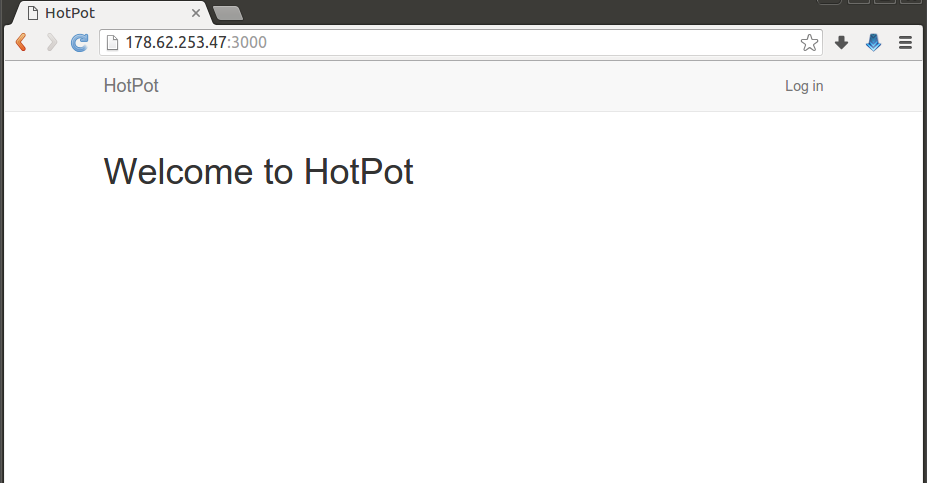
\includegraphics[width=1.0\linewidth]{gfx/chapter_5/general/homepage}
\caption[HotPot homepage]{HotPot homepage}
\label{fig:user_guide:homepage}
\end{figure}

\begin{figure}[bth]                                                                                                                                                  \myfloatalign
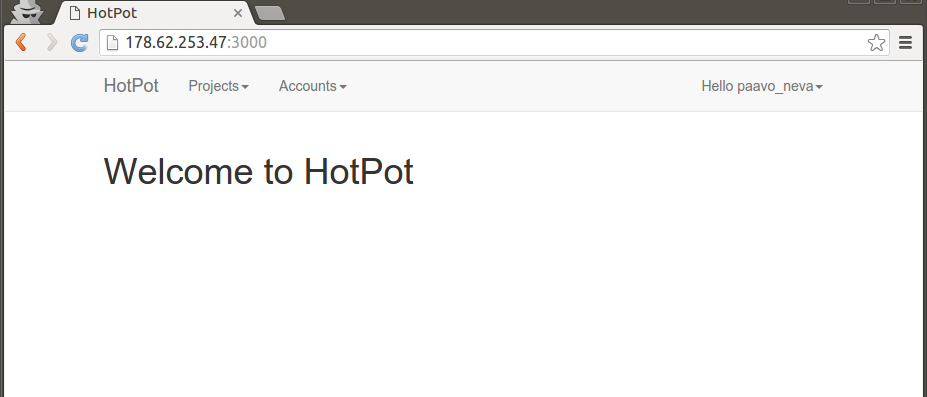
\includegraphics[width=1.0\linewidth]{gfx/chapter_5/general/user_interface}
\caption[HotPot user interface]{HotPot user interface}
\label{fig:user_guide:user_interface}
\end{figure}

\begin{figure}[bth]                                                                                                                                                  \myfloatalign
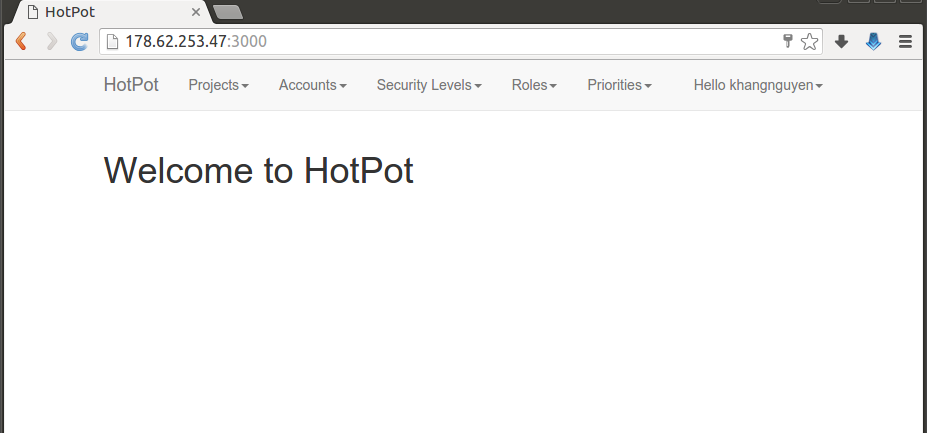
\includegraphics[width=1.0\linewidth]{gfx/chapter_5/general/admin_interface}
\caption[HotPot admin interface]{HotPot admin interface}
\label{fig:user_guide:admin_interface}
\end{figure}

\begin{figure}[bth]                                                                                                                                                  \myfloatalign
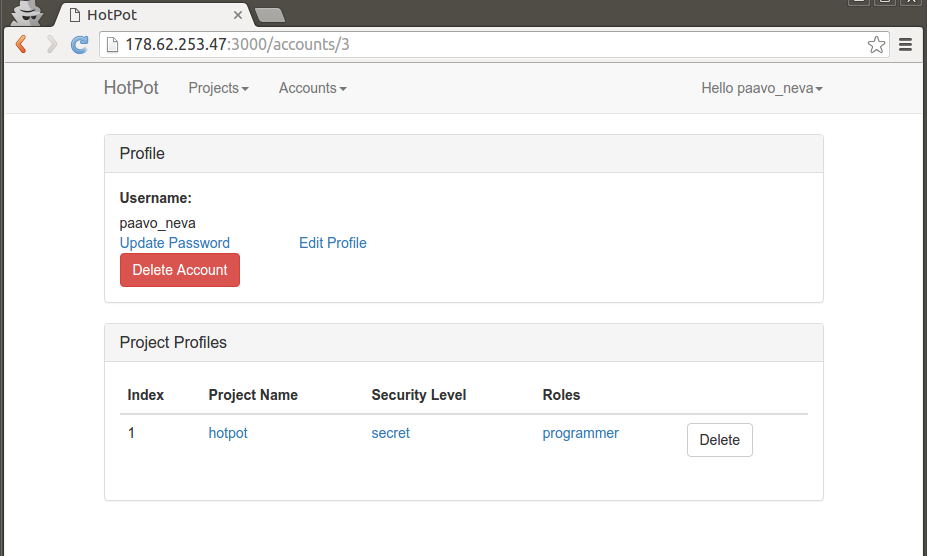
\includegraphics[width=1.0\linewidth]{gfx/chapter_5/general/profile}
\caption[HotPot profile page]{HotPot profile page}
\label{fig:user_guide:profile}
\end{figure}

\begin{figure}[bth]                                                                                                                                                  \myfloatalign
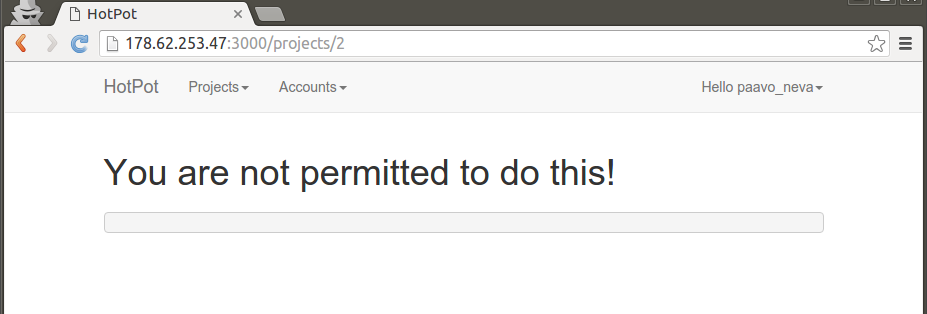
\includegraphics[width=1.0\linewidth]{gfx/chapter_5/general/not_permitted}
\caption[HotPot not permitted error]{HotPot not permitted error}
\label{fig:user_guide:not_permitted}
\end{figure}

\clearpage

\subsubsection{Login}
\label{ch:result:user_guide:miscellaneous:login}

\begin{description}
\item[Description] Every accounts can login to the system using its username and password.
\item[Parameters] An account whose username:password are:
\begin{itemize}
\item \emph{username}: paavo\_neva.
\item \emph{password}: paavo\_neva.
\end{itemize}
\item[Results] If the account is authenticated then a token is created and save on client cookies, and the user is redirected to homepage.
If the account is invalid, the login page will be rendered with error messages.
\end{description}

On homepage \autoref{fig:user_guide:homepage} click on \emph{Log in} link on the top bar to go to \href{http://178.62.253.47:3000/login}{http://178.62.253.47:3000/login}.

\begin{figure}[bth]                                                                                                                                                  \myfloatalign
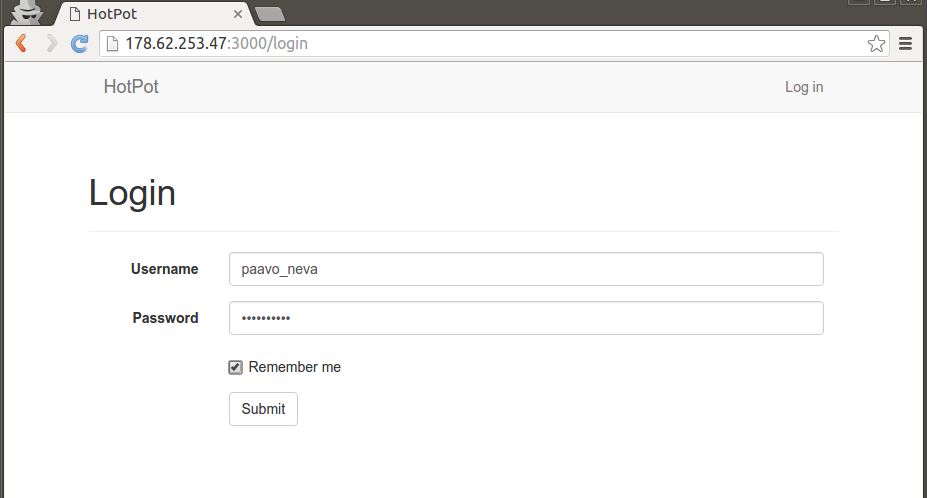
\includegraphics[width=1.0\linewidth]{gfx/chapter_5/miscellaneous/login}
\caption[HotPot login page]{HotPot login page}
\label{fig:user_guide:miscellaneous:login}
\end{figure}

\begin{figure}[bth]
\myfloatalign
\subfloat[Login failed]
{
\label{fig:user_guide:miscellaneous:login_failed}
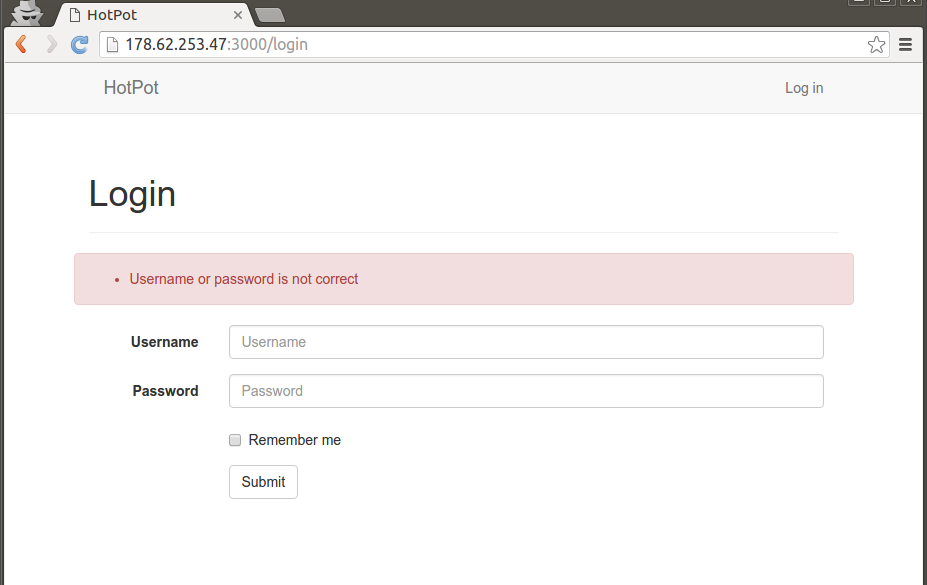
\includegraphics[width=1.\linewidth]{gfx/chapter_5/miscellaneous/login_failed}
} \quad
\subfloat[Login successfully then redirected to profile page]
{
\label{fig:user_guide:miscellaneous:profile}
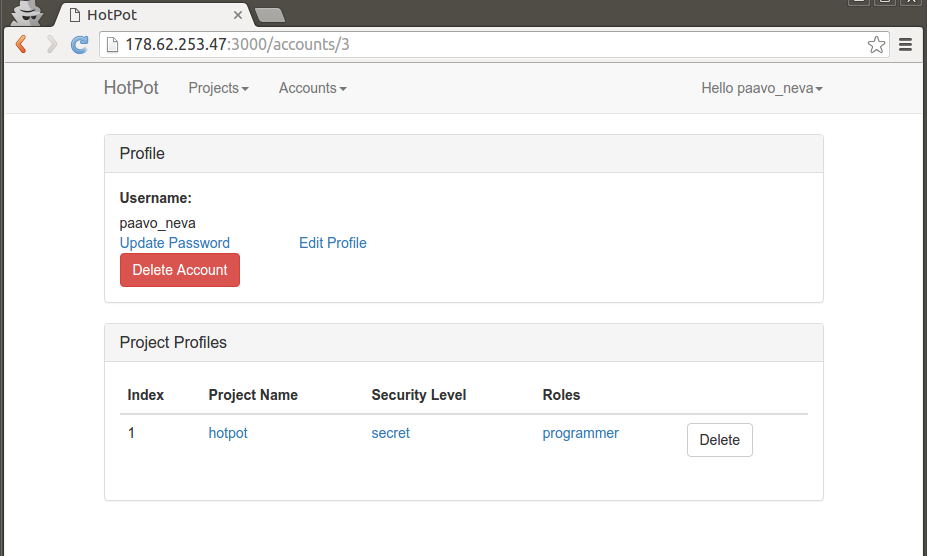
\includegraphics[width=1.\linewidth]{gfx/chapter_5/general/profile}
} \\
\caption[Login results]{Login results}
\label{fig:user_guide:login:result}
\end{figure}

\clearpage

\subsubsection{Logout}
\label{ch:result:user_guide:miscellaneous:logout}

\begin{description}
\item[Description] Every logged in accounts can logout from the system.
\item[Parameters] A logged in account.
\item[Results] The account will be logged out.
Its token will be deleted.
All of his cookies data on the client will be emptied.
Finally, he will be redirected to homepage.
\end{description}

After logging in, on any pages, click on the username link to show \emph{Log out} link.
Click on it for logging out.
After that, the user will be redirected to \emph{homepage} \(\autoref{fig:user_guide:homepage}\).

\begin{figure}[bth]                                                                                                                                                  \myfloatalign
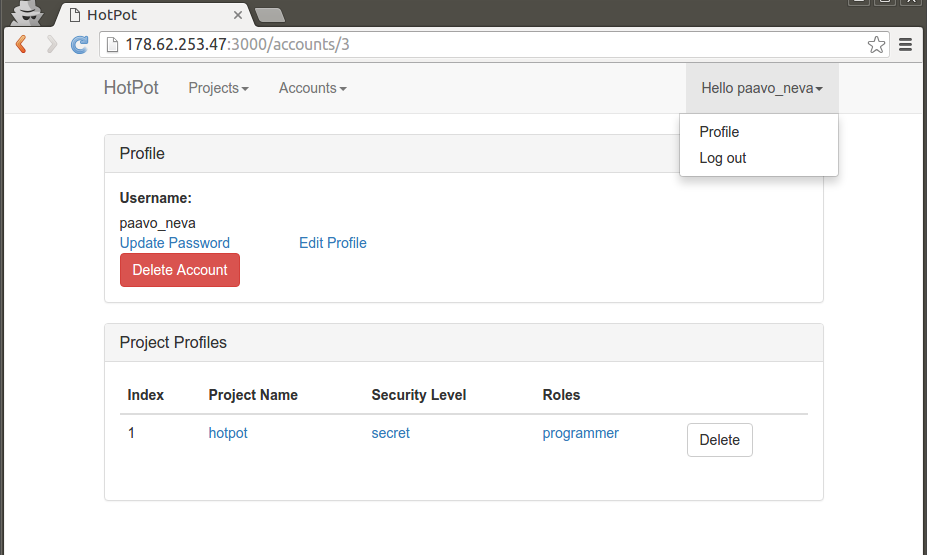
\includegraphics[width=1.0\linewidth]{gfx/chapter_5/miscellaneous/logout}
\caption[HotPot logout link]{HotPot logout link}
\label{fig:user_guide:miscellaneous:logout}
\end{figure}

%\clearpage

% Account guide ----------------------------
\subsection{Account}
\label{ch:result:user_guide:account}
\subsubsection{Create}
\label{ch:result:user_guide:account:create}

\begin{description}
\item[Description] Administrators can create new accounts on the system.
\item[Pre-conditions] An administrator account is logged in.
\item[Parameters] Create an account with values:
\begin{itemize}
\item \emph{username}: testingtesting.
\item \emph{password}: testingtesting.
\end{itemize}
\item[Results] If all the input information is valid, new account will be created, otherwise error messages will be displayed.
\end{description}

After logging in as an administrator, the user interface will appeared like in \autoref{fig:user_guide:admin_interface}.
On the tool bar, click on \emph{Accounts}, then \emph{Create account}.
The creating page will appear under URL

\noindent\href{http://178.62.253.47:3000/accounts/create}{http://178.62.253.47:3000/accounts/create} as shown in \autoref{fig:user_guide:account:account_create}.
Input the value, the \emph{Confirm Password} field is for re-typing password, and the result will be shown as \autoref{fig:user_guide:account:account_create_result}.

\begin{figure}[bth]
\myfloatalign
\subfloat[HotPot Account creation link]
{
\label{fig:user_guide:account:account_create_link}
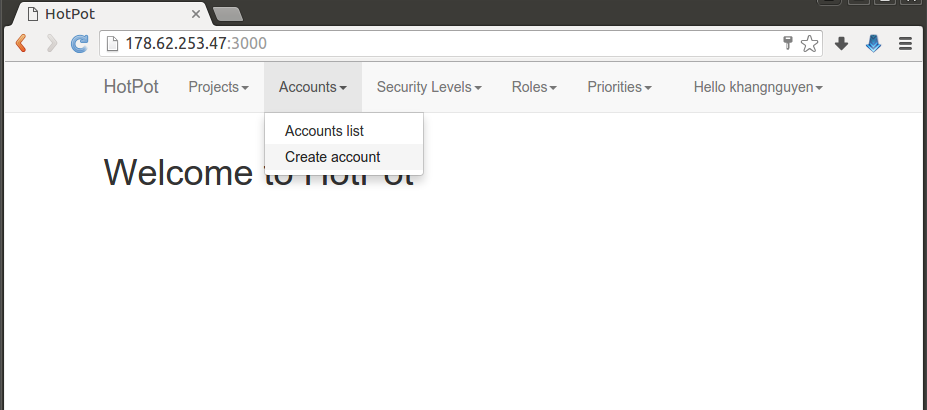
\includegraphics[width=1.0\linewidth]{gfx/chapter_5/account/account_create_link}
} \quad
\subfloat[HotPot Account creating page]
{
\label{fig:user_guide:account:account_create}
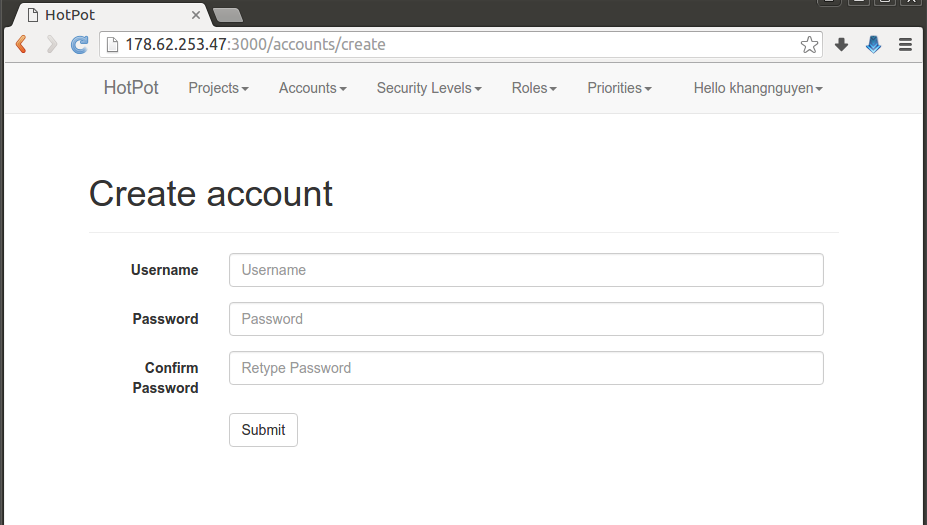
\includegraphics[width=1.0\linewidth]{gfx/chapter_5/account/account_create}
} \\
\caption[HotPot Account creation]{HotPot Account creating}
\label{fig:user_guide:account:account_create}
\end{figure}

\begin{figure}[bth]
\myfloatalign
\subfloat[Account creating failed]
{
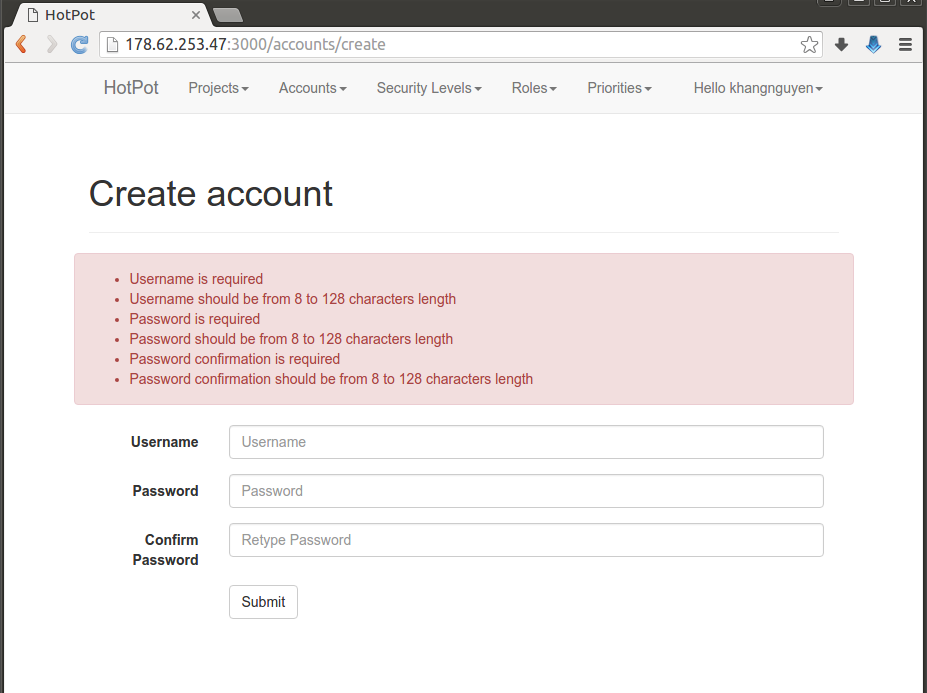
\includegraphics[width=1.\linewidth]{gfx/chapter_5/account/account_create_failed}
} \quad
\subfloat[Account creating successfully then redirected to account detail page]
{
\label{fig:user_guide:account:account_view}
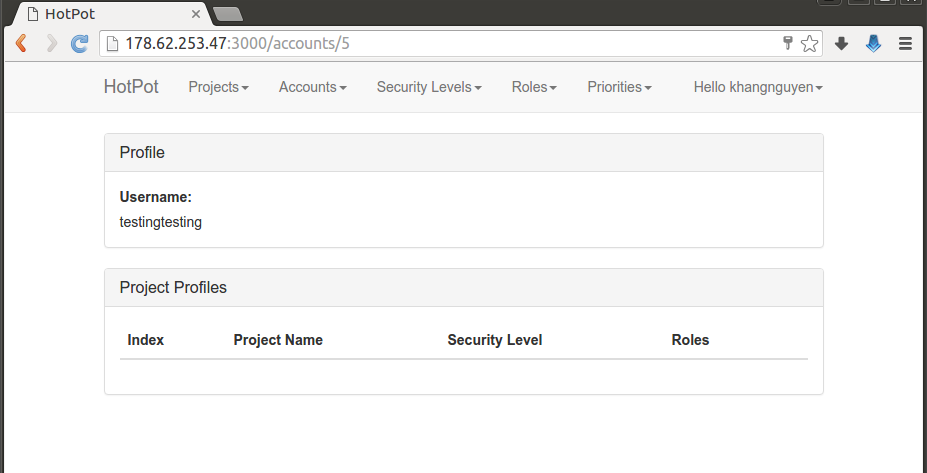
\includegraphics[width=1.\linewidth]{gfx/chapter_5/account/account_view}
} \\
\caption[Login results]{Account creating results}
\label{fig:user_guide:account:account_create_result}
\end{figure}

\clearpage

\subsubsection{Edit profile}
\label{ch:result:user_guide:account:profile}

\begin{description}
\item[Description] Account's owner can edit his all profile details.
\item[Pre-conditions] An account is logged in.
\item[Parameters] Update the logged in account's profile with values:
\begin{itemize}
\item \emph{fullname}: Paavo Neva.
\item \emph{email}: paavo@hotpot.com.
\end{itemize}
\item[Results] If all the input information is valid, the account's profile will be updated.
\end{description}

After logging in, the user interface will appeared like in \autoref{fig:user_guide:user_interface}.
On the tool bar, click on the account name on left top corner, then \emph{Profile} as shown in \autoref{fig:user_guide:account:profile_link}.
The account's profile page will appear under URL \href{http://178.62.253.47:3000/accounts/3}{http://178.62.253.47:3000/accounts/3} as shown in \autoref{fig:user_guide:profile}.
Click on \emph{Edit Profile} link, to go to \href{http://178.62.253.47:3000/accounts/update\_detail}{http://178.62.253.47:3000/accounts/update\_detail} as shown in 
\autoref{fig:user_guide:account:edit_profile}
Input the value, and the result will be shown as \autoref{fig:user_guide:account:profile_updated}.

\begin{figure}[bth]
\myfloatalign
\subfloat[HotPot Profile update link]
{
\label{fig:user_guide:account:profile_link}
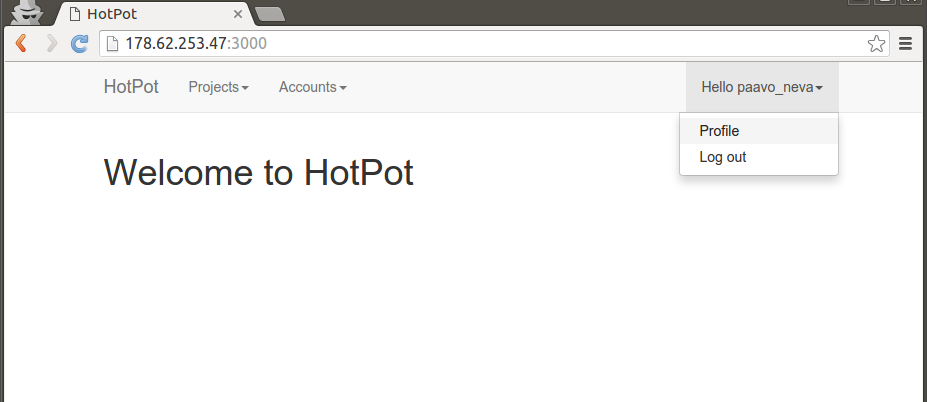
\includegraphics[width=1.0\linewidth]{gfx/chapter_5/account/profile_link}
} \quad
\subfloat[HotPot Profile editing page]
{
\label{fig:user_guide:account:edit_profile}
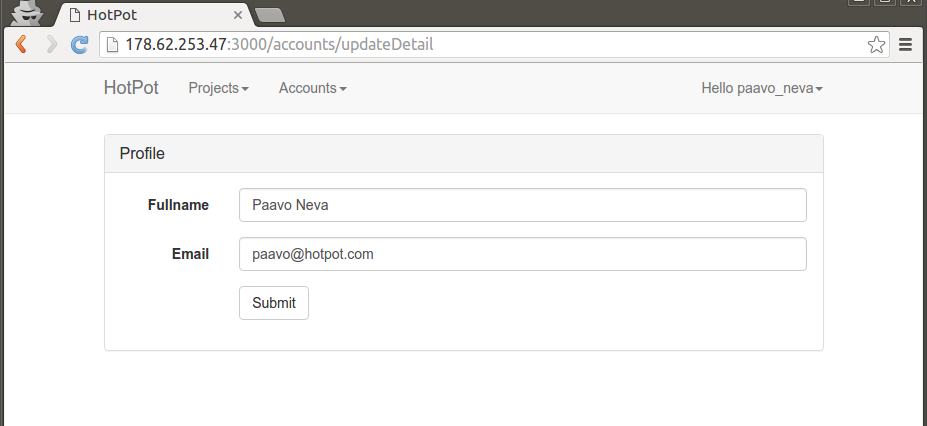
\includegraphics[width=1.0\linewidth]{gfx/chapter_5/account/edit_profile}
} \\
\caption[HotPot Account creation]{HotPot Account creating}
\label{fig:user_guide:account:edit_profile}
\end{figure}

\begin{figure}[bth]                                                                                                                                                  \myfloatalign
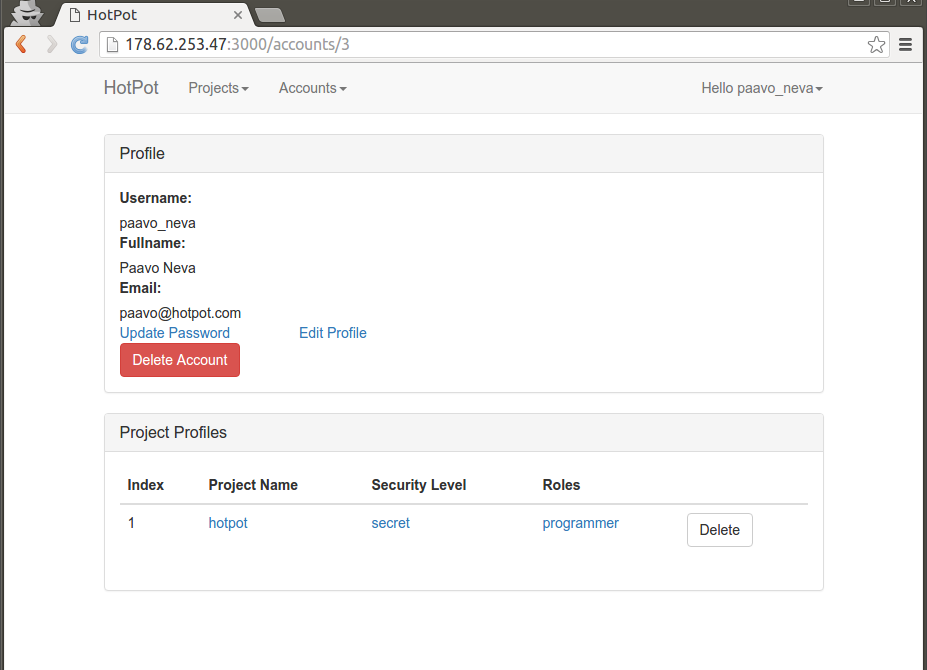
\includegraphics[width=1.0\linewidth]{gfx/chapter_5/account/profile_updated}
\caption[HotPot Profile updated]{HotPot Profile updated}
\label{fig:user_guide:account:profile_updated}
\end{figure}

\subsubsection{Change Password}
\label{ch:result:user_guide:account:change_password}

\begin{description}
\item[Description] Account's owner can change his password.
\item[Pre-conditions] An account is logged in.
\item[Parameters] Update the logged in account's password with values:
\begin{itemize}
\item \emph{password}: newpasswordupdate.
\end{itemize}
\item[Results] If the new password is valid, the user will be redirected back to his profile page.
\end{description}

On user's profile page \(\autoref{fig:user_guide:profile}\), click \emph{Update Password} to go to \href{http://178.62.253.47:3000/accounts/update\_password}{http://178.62.253.47:3000/accounts/update\_password}.
Input new password.
If the new password is valid, the user will be redirected to \autoref{fig:user_guide:profile}, otherwise error messages will be shown as \autoref{fig:user_guide:account:change_password_failed}.

\begin{figure}[bth]
\myfloatalign
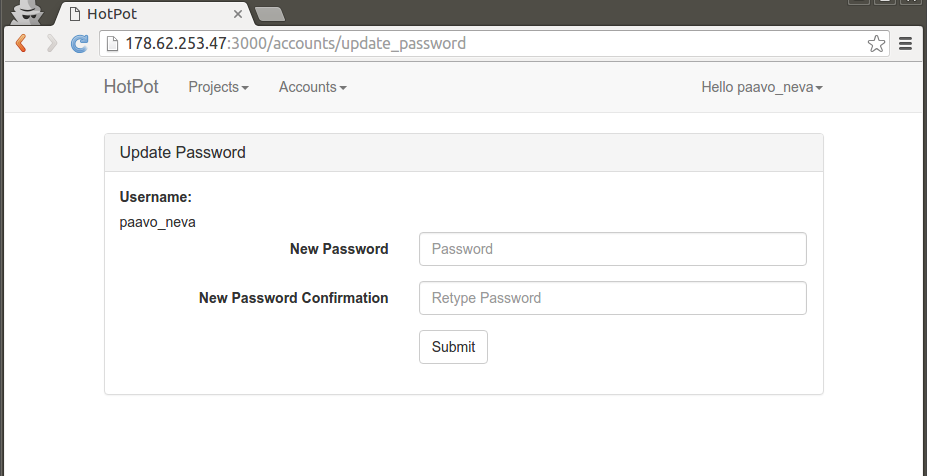
\includegraphics[width=1.0\linewidth]{gfx/chapter_5/account/change_password}
\caption[HotPot password changing page]{HotPot password changing page}
\label{fig:user_guide:account:change_password}
\end{figure}

\begin{figure}[bth]                                                                                                                                                  \myfloatalign
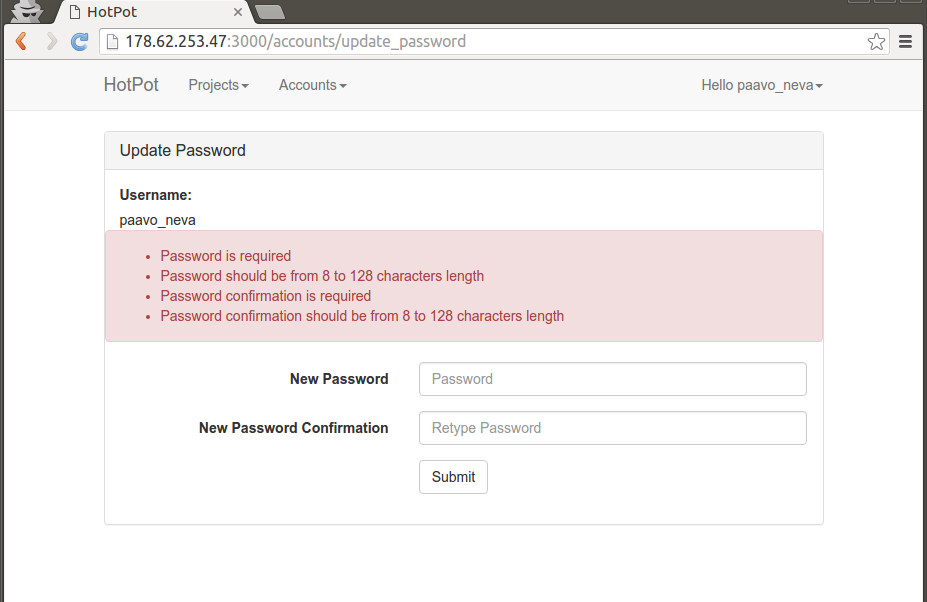
\includegraphics[width=1.0\linewidth]{gfx/chapter_5/account/change_password_failed}
\caption[Password changing failed]{Password changing failed}
\label{fig:user_guide:account:change_password_failed}
\end{figure}

\clearpage

\subsubsection{Delete}
\label{ch:result:user_guide:account:delete}

\begin{description}
\item[Description] Account's owner can delete his account.
\item[Pre-conditions] An account is logged in.
\item[Results] The account will be deleted from the system.
\end{description}

On profile page \autoref{fig:user_guide:profile}, click on \emph{Delete Account} button.

\subsubsection{List and View}
\label{ch:result:user_guide:account:list}

\begin{description}
\item[Description] Every accounts can view the accounts list and their profile.
\item[Pre-conditions] An account is logged in.
\end{description}

On any pages, click on \emph{Accounts} link on top bar, then click on \emph{Account list} link to go to \href{http://178.62.253.47:3000/accounts}{http://178.62.253.47:3000/accounts} as shown in \autoref{fig:user_guide:account:account_list}.
Then, clicking on any user's name to go to account view, as shown in \autoref{fig:user_guide:account:account_view}.

\begin{figure}[bth]
\myfloatalign
\subfloat[HotPot Account list link]
{
\label{fig:user_guide:account:list_link}
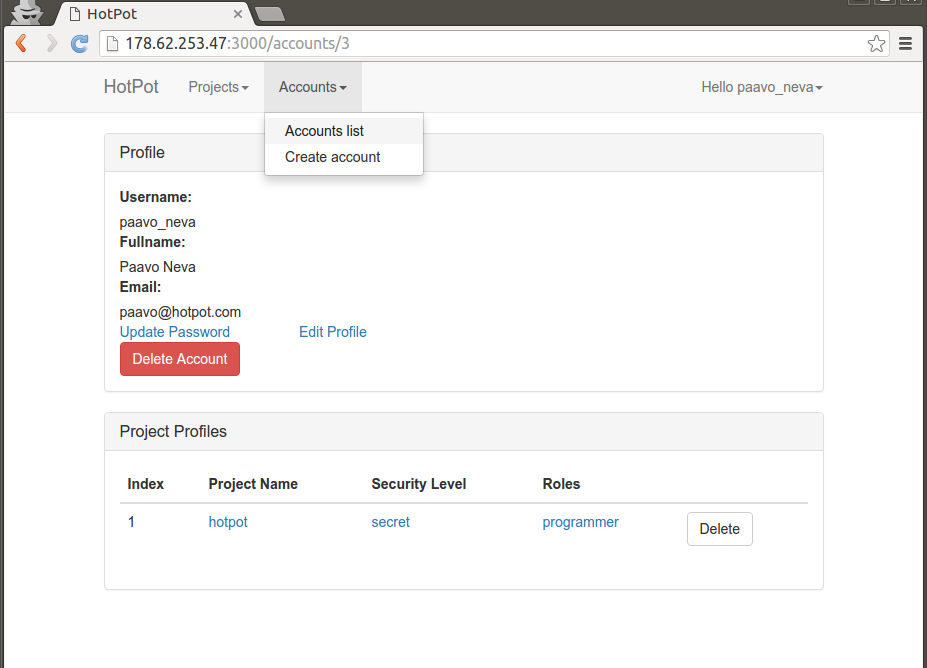
\includegraphics[width=1.0\linewidth]{gfx/chapter_5/account/account_list_link}
} \quad
\subfloat[HotPot Account list page]
{
\label{fig:user_guide:account:account_list}
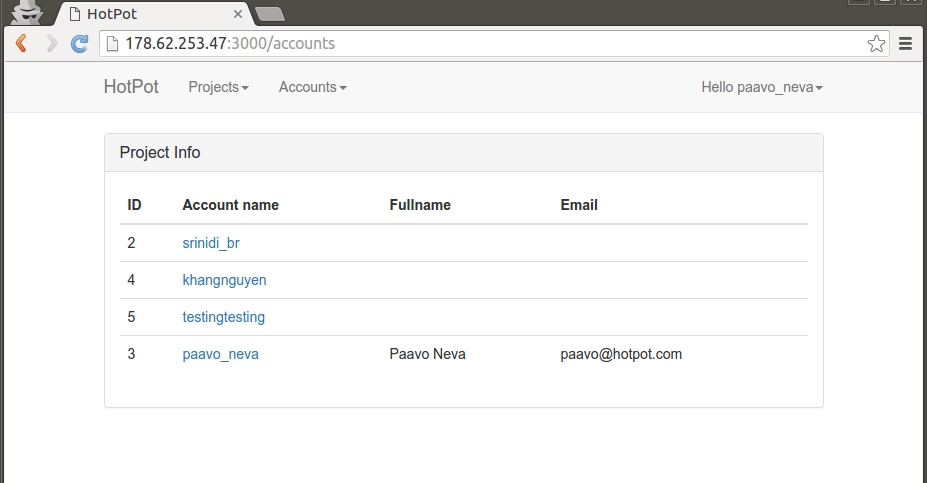
\includegraphics[width=1.0\linewidth]{gfx/chapter_5/account/account_list}
} \\
\caption[HotPot Account list]{HotPot Account list}
\label{fig:user_guide:account:account_list}
\end{figure}

\clearpage

% Project guide ----------------------------
\subsection{Project}
\label{ch:result:user_guide:project}
\subsubsection{Create}
\label{ch:result:user_guide:project:create}

\begin{description}
\item[Description] Every account can create a new project.
\item[Pre-conditions] A logged in account.
\item[Parameters] Create an project with values:
\begin{itemize}
\item \emph{name}: Paavo Project.
\item \emph{description}:  This project is created by paavo\_neva.
\item \emph{due date}: 02/29/2016.
\end{itemize}
\item[Results] If all the input information is valid, new project will be created, the account will be marked as its owner, and the owner will be its first member.
\end{description}

After logging in, on the tool bar, click on \emph{Projects}, then \emph{Create project} as shown in as shown in \autoref{fig:user_guide:project:project_create_link}.
The creating page will appear under URL \href{http://178.62.253.47:3000/projects/create}{http://178.62.253.47:3000/projects/create} as shown in \autoref{fig:user_guide:project:project_create}.
Input the value and the result will be shown as \autoref{fig:user_guide:project:project_create_result}.

\begin{figure}[bth]
\myfloatalign
\subfloat[HotPot Project creation link]
{
\label{fig:user_guide:project:project_create_link}
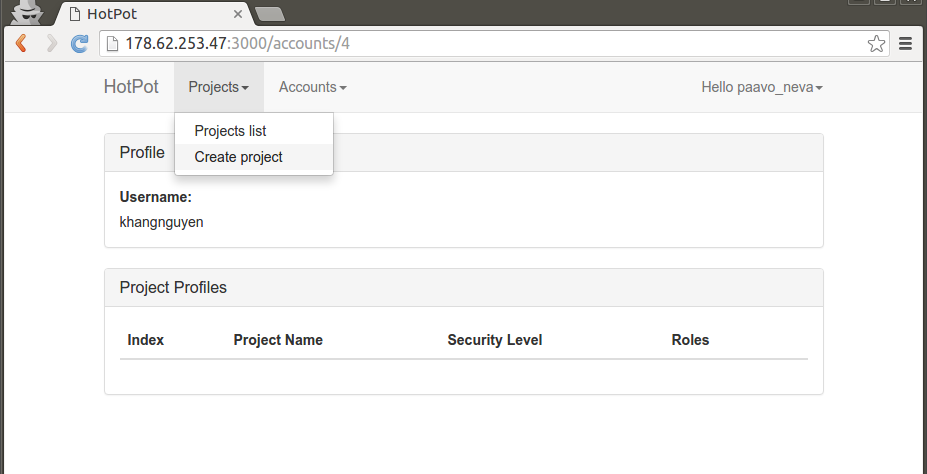
\includegraphics[width=1.0\linewidth]{gfx/chapter_5/project/project_create_link}
} \quad
\subfloat[HotPot Project creating page]
{
\label{fig:user_guide:project:project_create}
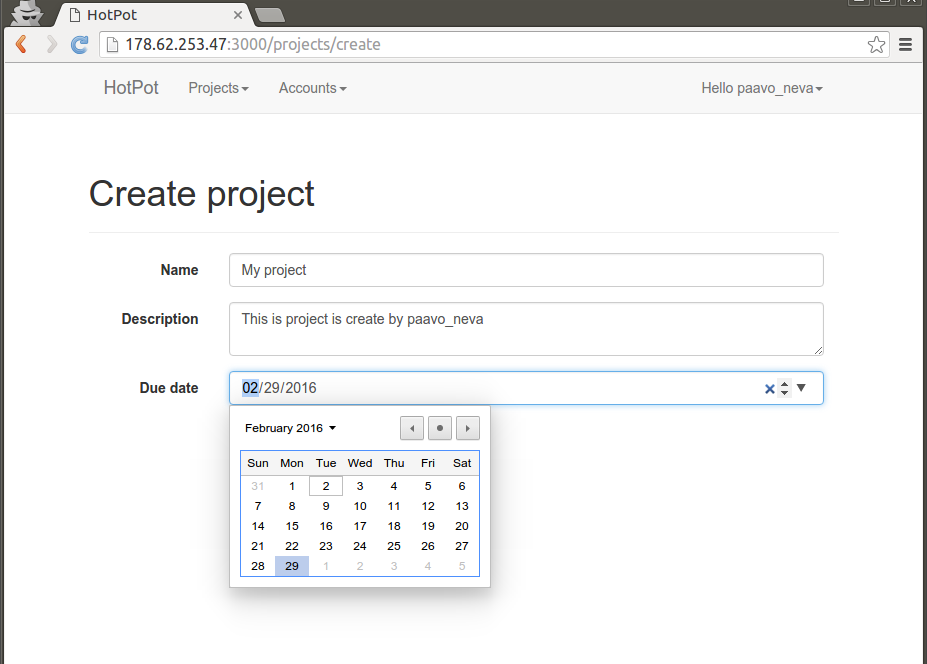
\includegraphics[width=1.0\linewidth]{gfx/chapter_5/project/project_create}
} \\
\caption[HotPot Project creation]{HotPot Project creating}
\label{fig:user_guide:project:project_create}
\end{figure}

\begin{figure}[bth]
\myfloatalign
\subfloat[Project creating failed]
{
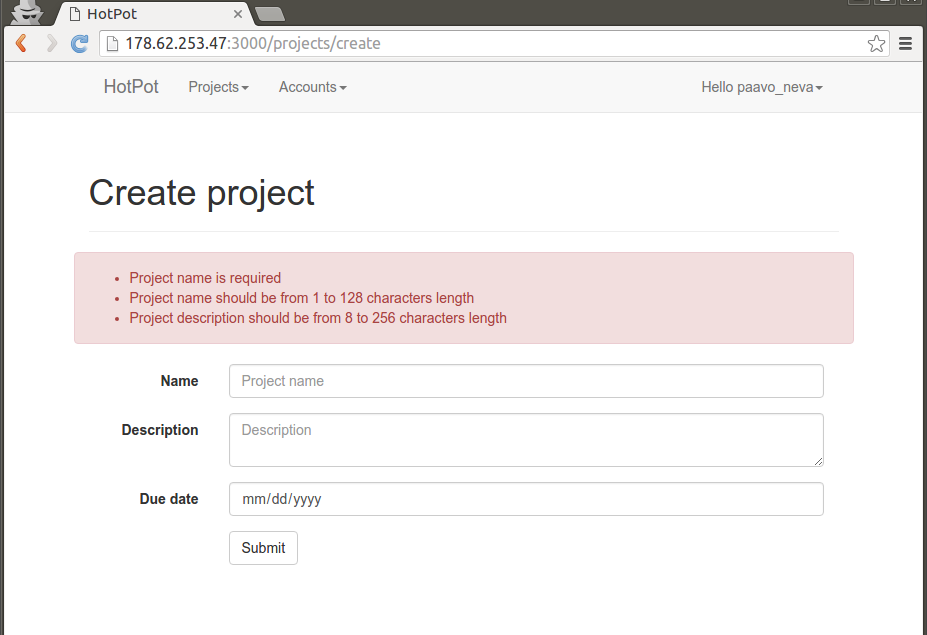
\includegraphics[width=1.\linewidth]{gfx/chapter_5/project/project_create_failed}
} \quad
\subfloat[Project creating successfully then redirected to project detail page]
{
\label{fig:user_guide:project:project_view}
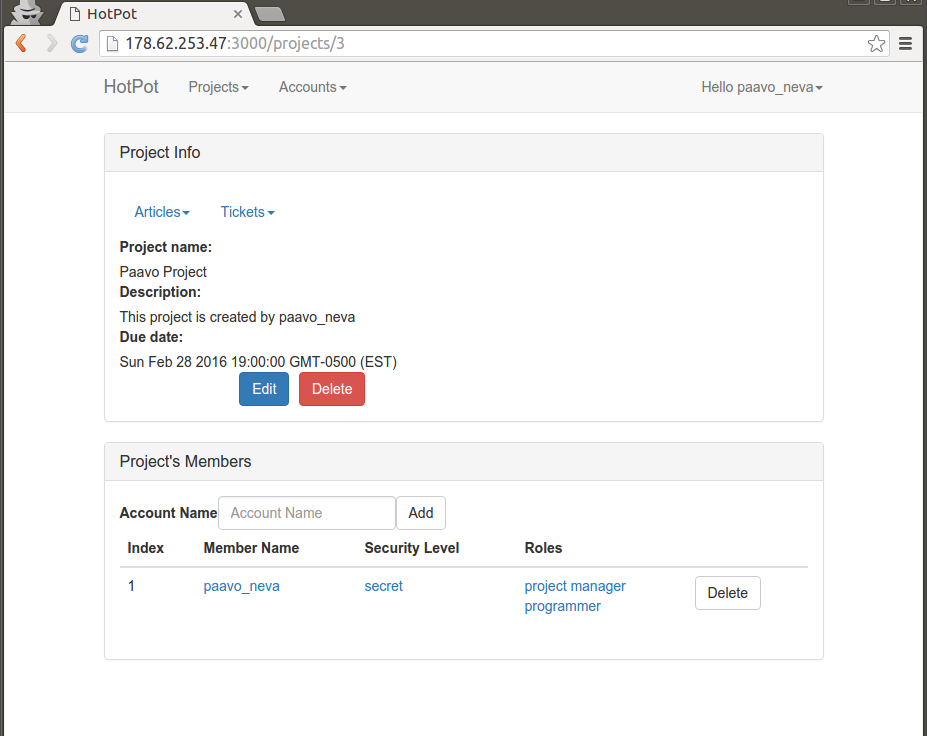
\includegraphics[width=1.\linewidth]{gfx/chapter_5/project/project_view}
} \\
\caption[Project creating results]{Project creating results}
\label{fig:user_guide:project:project_create_result}
\end{figure}

\clearpage

\subsubsection{Managing member}
\label{ch:result:user_guide:project:managing_member}

\begin{description}
\item[Description] Only project owner can add or remove project's member.
\item[Pre-conditions] Project's owner logged in, \eg account \emph{paavo\_neva}.
\item[Parameters] Add and remove user \emph{srinidi\_br} to/from \emph{Paavo Project} project.
\item[Results] The account will respectively be added and removed from \emph{Paavo Project} project.
\end{description}

After logging in as the project's owner, go to his own project in URL \href{http://178.62.253.47:3000/projects/3}{http://178.62.253.47:3000/projects/3}.
Input the \emph{account's name} and the result will be shown as \autoref{fig:user_guide:project:assign_member}.

For removing project's member, on the project view, click on the member's \emph{Delete} button.

\begin{figure}[bth]
\myfloatalign
\subfloat[Project: inputting project's new member username]
{
\label{fig:user_guide:project:input_new_member}
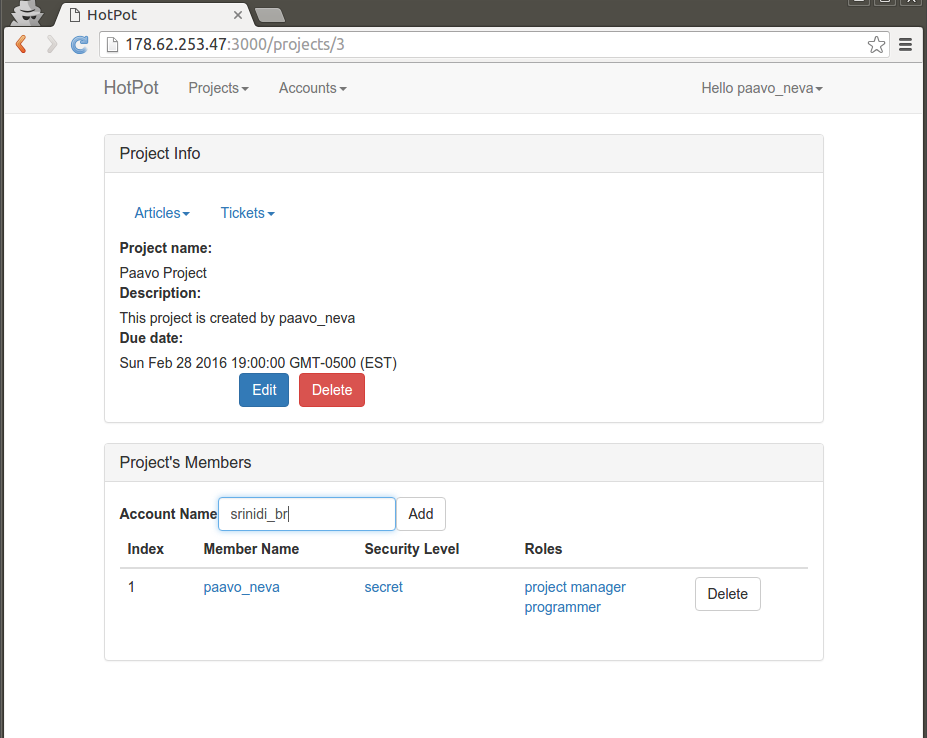
\includegraphics[width=1.\linewidth]{gfx/chapter_5/project/assign_member}
} \quad
\subfloat[Project: assigning project's new member successfully]
{
\label{fig:user_guide:project:project_view}
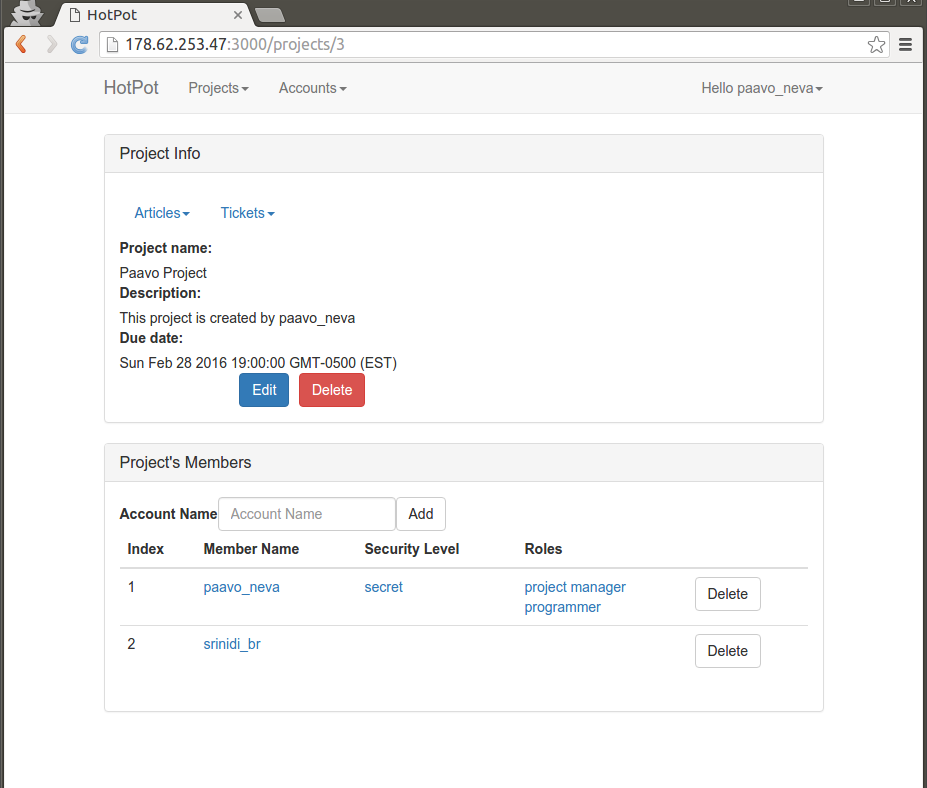
\includegraphics[width=1.\linewidth]{gfx/chapter_5/project/assign_member_successfully}
} \\
\caption[Project: assigning project's new member]{Project: assigning project's new member}
\label{fig:user_guide:project:assign_member}
\end{figure}

\clearpage

\subsubsection{Update}
\label{ch:result:user_guide:project:update}

\begin{description}
\item[Description] Only project owner can edit his own project.
\item[Pre-conditions] Project's owner logged in, \eg account \emph{paavo\_neva}.
\item[Results] The project will be updated with new details.
\end{description}

After logging in as the project's owner, on the project view page, as shown in \autoref{fig:user_guide:project:project_view}, click \emph{Edit} button to go to its edit page 

\noindent\href{http://178.62.253.47:3000/projects/edit/3}{http://178.62.253.47:3000/projects/edit/3}.
Change the project's details.
If there are any errors, they will be shown as \autoref{fig:user_guide:project:project_edit_failed}, otherwise the user will be redirected to project view.

\begin{figure}[bth]
\myfloatalign
\subfloat[Project: edit page]
{
\label{fig:user_guide:project:project_edit_page}
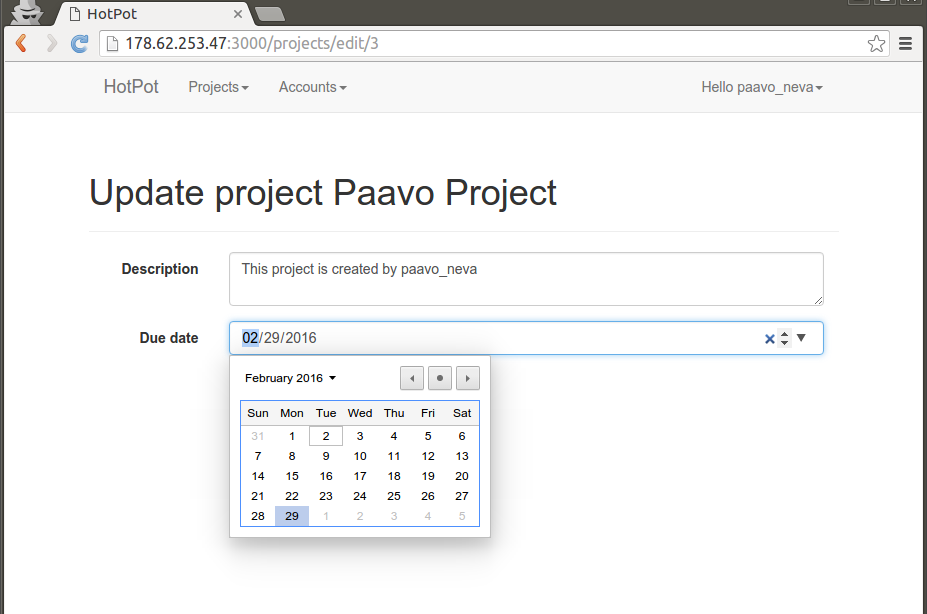
\includegraphics[width=1.\linewidth]{gfx/chapter_5/project/project_edit}
} \quad
\subfloat[Project: project editing failed]
{
\label{fig:user_guide:project:project_edit_failed}
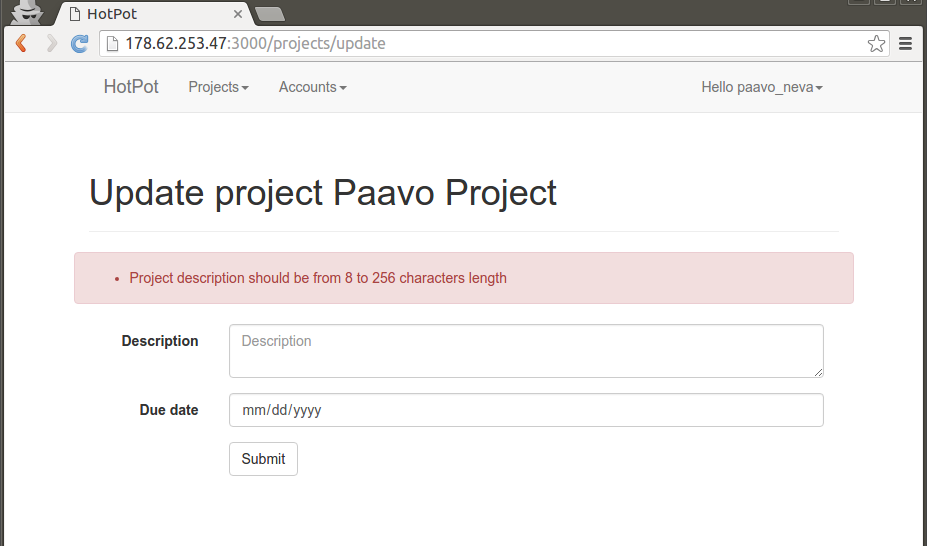
\includegraphics[width=1.\linewidth]{gfx/chapter_5/project/project_edit_failed}
} \\
\caption[Project: project edit]{Project:  project edit}
\label{fig:user_guide:project:project_edit}
\end{figure}

\clearpage

\subsubsection{Delete}
\label{ch:result:user_guide:project:delete}

\begin{description}
\item[Description] Only project owner can delete his own project.
\item[Pre-conditions] Project's owner logged in, \eg account \emph{paavo\_neva}.
\item[Results] The project will be deleted.
\end{description}

After logging in as the project's owner, on the project view page, as shown in \autoref{fig:user_guide:project:project_view}, click \emph{Delete} button to delete the current project. 

\subsubsection{List and View}
\label{ch:result:user_guide:project:list}

\begin{description}
\item[Description] Every accounts can view the list of projects. However, only the team member can view the project's details.
\item[Pre-conditions] A logged in account, \eg account \emph{paavo\_neva}.
\item[Results] The user can view the list of all projects, but can only see details of projects in which he is a team member.
\end{description}

After logging in, in every pages, on the top bar, click on \emph{Projects} link, then click on \emph{Projects list}, as shown in \autoref{fig:user_guide:project:project_list_link}, to go to 

\noindent\href{http://178.62.253.47:3000/projects}{http://178.62.253.47:3000/projects} as shown in \autoref{fig:user_guide:project:project_list}.
Then clicking on any project's name will go to the project's view page, as \autoref{fig:user_guide:project:project_view}, if the user is a member of the project, otherwise \autoref{fig:user_guide:not_permitted} will be shown.

\begin{figure}[bth]
\myfloatalign
\subfloat[Project: projects list link]
{
\label{fig:user_guide:project:project_list_link}
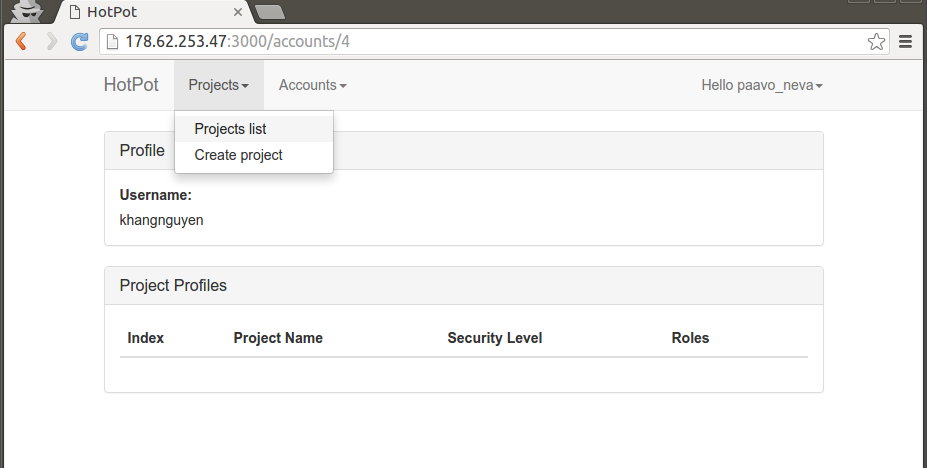
\includegraphics[width=1.\linewidth]{gfx/chapter_5/project/project_list_link}
} \quad
\subfloat[Project: projects list]
{
\label{fig:user_guide:project:project_list}
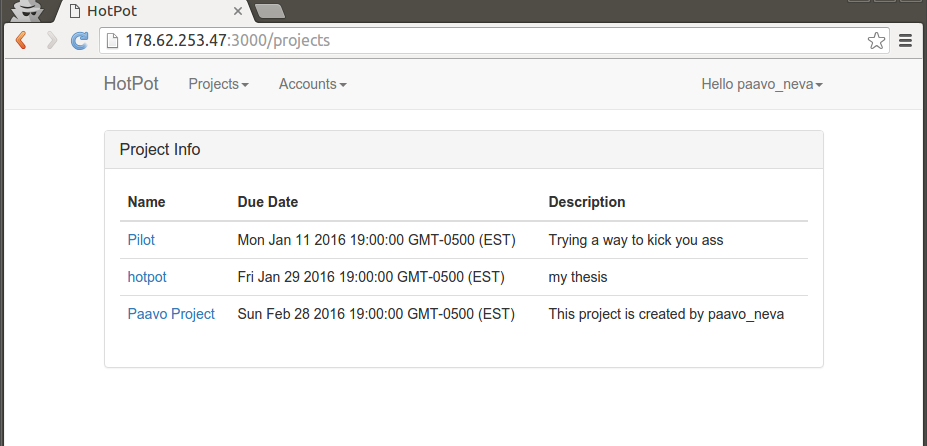
\includegraphics[width=1.\linewidth]{gfx/chapter_5/project/project_list}
} \\
\caption[Project: view projects list]{Project: view projects list}
\label{fig:user_guide:project:project_list}
\end{figure}

\clearpage

% Article guide ----------------------------
\subsection{Article}
\label{ch:result:user_guide:article}
\subsubsection{Create}
\label{ch:result:user_guide:article:create}

\begin{description}
\item[Description] Only project members can create the project's new articles.
\item[Pre-conditions] Project's member logged in, \eg account \emph{paavo\_neva} and project \emph{Paavo Project}.
\item[Conditions] The article's \emph{security level} can only be equal or higher than its creator's.
\item[Parameters] Create new article with these values:
\begin{itemize}
\item \emph{name}: Paavo article.
\item \emph{description}: This article is created by Paavo.
\item \emph{content}: A secret content.
\item \emph{is directory}: false.
\item \emph{writable}: true.
\item \emph{readable}: true.
\item \emph{security level}: secret (equals to account \emph{paavo\_neva}).
\item \emph{role}: designer and programmer.
\end{itemize}
\item[Results] A new artilce will be created under the project.
\end{description}

On the project's view page, click on \emph{Articles} link, then click on \emph{Create article}, as shown in \autoref{fig:user_guide:article:article_create}, to go to \href{http://178.62.253.47:3000/articles/create}{http://178.62.253.47:3000/articles/create}.
Input the article's information.
If the inputs are valid, a new article will be created and the user will be redirected to the article view page as \autoref{fig:user_guide:article:article_view}.
Otherwise, error messages will be displayed as \autoref{fig:user_guide:article:article_create_failed}

\begin{figure}[bth]
\myfloatalign
\subfloat[Article: articles create link]
{
\label{fig:user_guide:article:article_create_link}
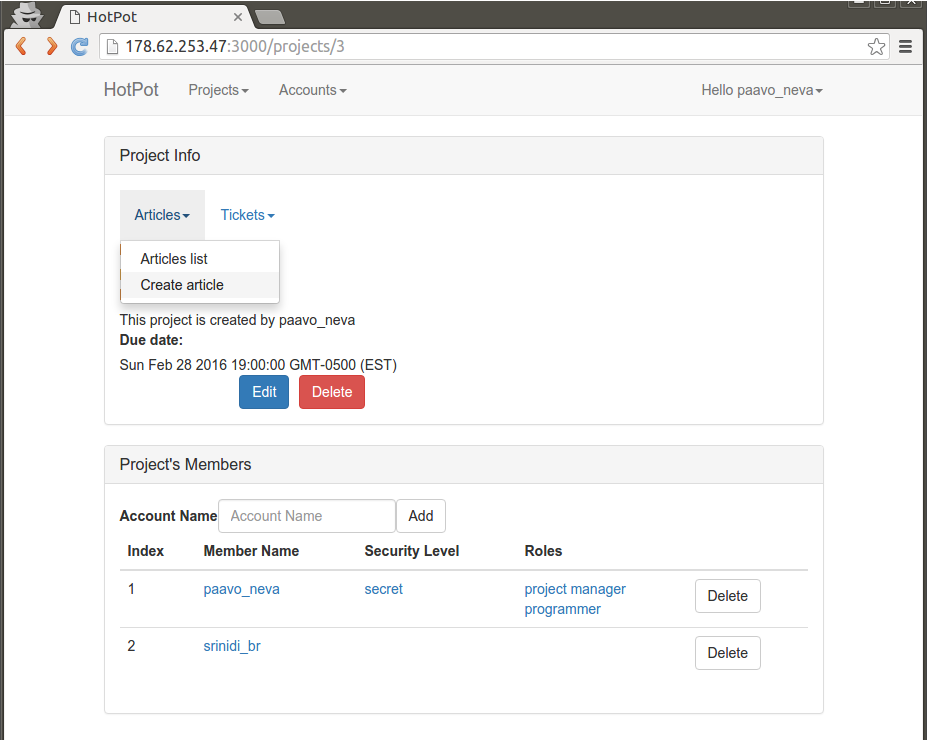
\includegraphics[width=1.\linewidth]{gfx/chapter_5/article/article_create_link}
} \quad
\subfloat[Article: articles create page]
{
\label{fig:user_guide:article:article_create}
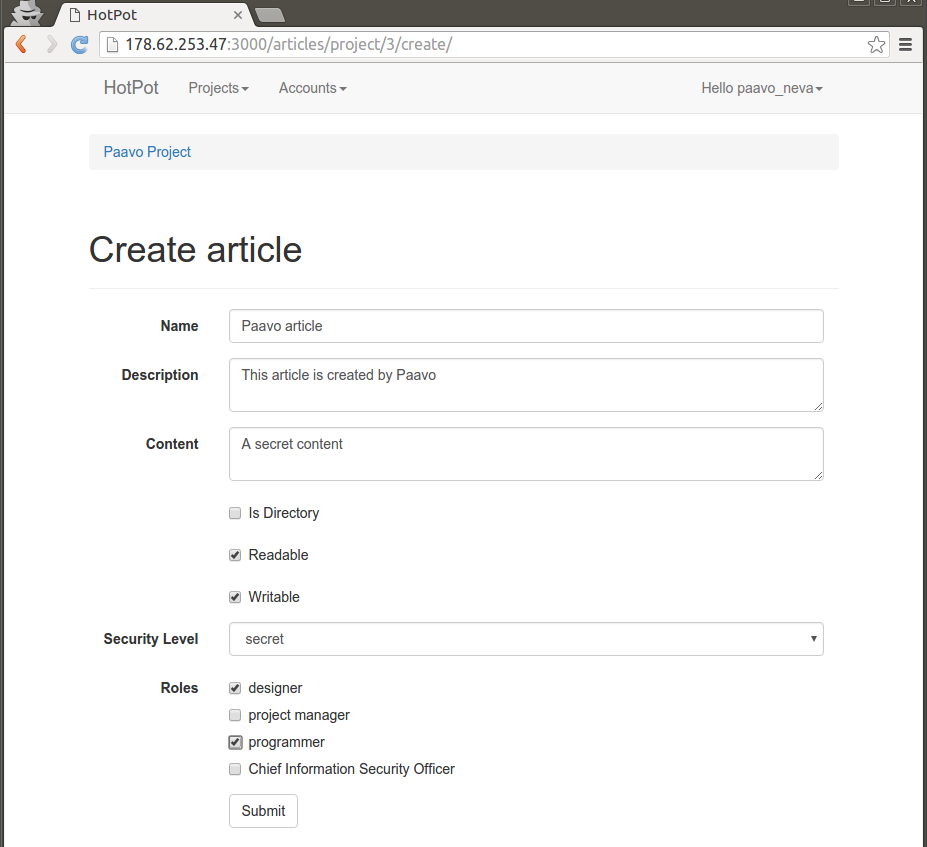
\includegraphics[width=1.\linewidth]{gfx/chapter_5/article/article_create}
} \\
\caption[Article: create articles]{Article: create articles}
\label{fig:user_guide:article:article_create}
\end{figure}

\begin{figure}[bth]
\myfloatalign
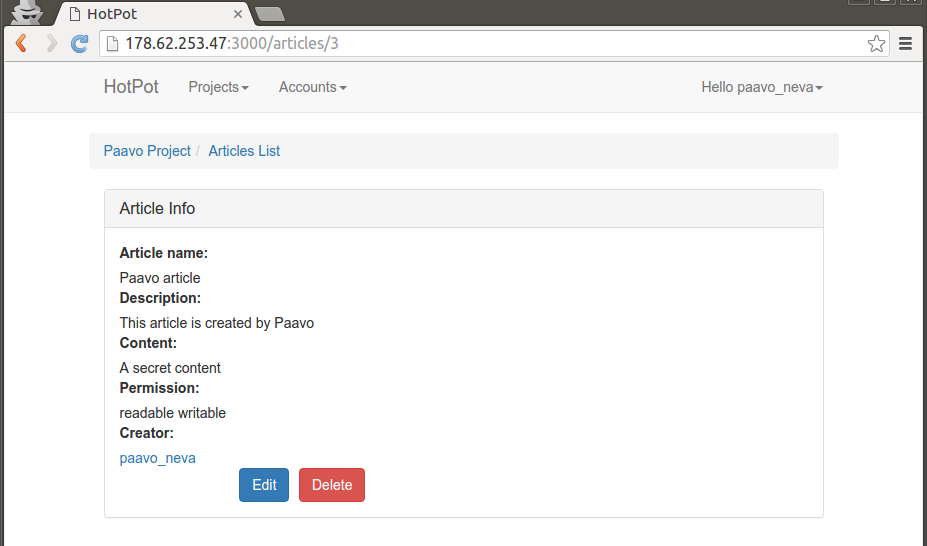
\includegraphics[width=1.0\linewidth]{gfx/chapter_5/article/article_view}
\caption[Article: article view page]{Article: article view page}
\label{fig:user_guide:article:article_view}
\end{figure}

\begin{figure}[bth]
\myfloatalign
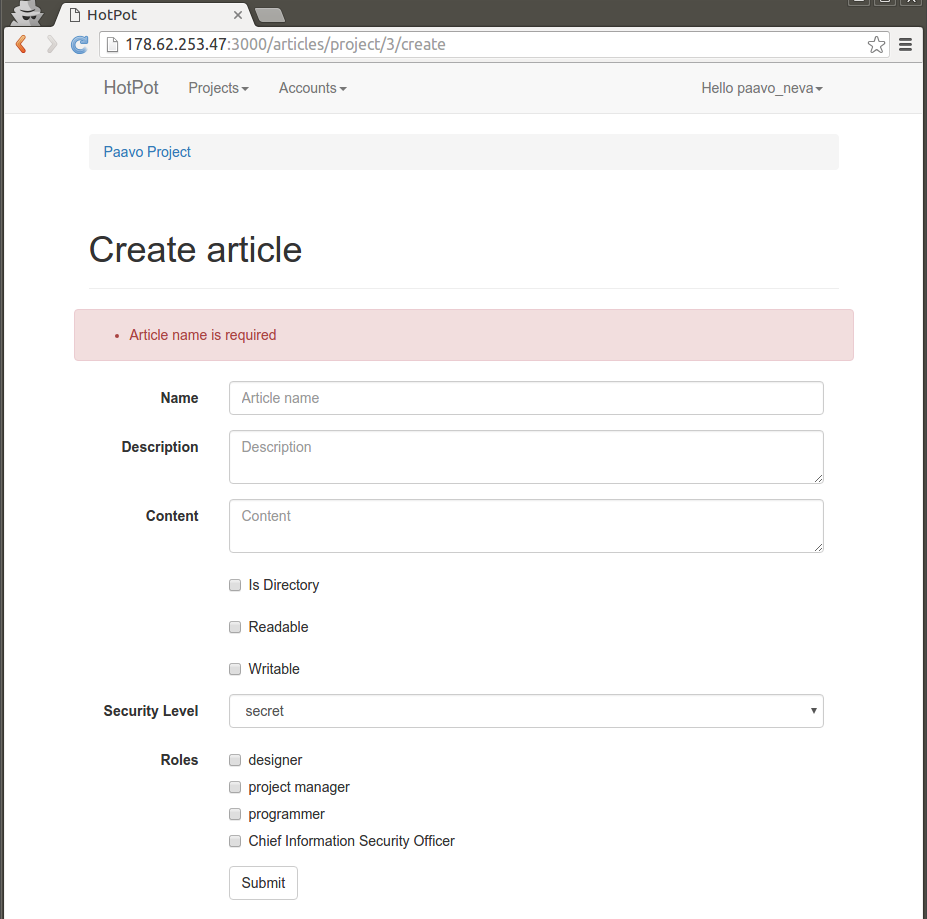
\includegraphics[width=1.0\linewidth]{gfx/chapter_5/article/article_create_failed}
\caption[Article: article list]{Article: article creating failed}
\label{fig:user_guide:article:article_create_failed}
\end{figure}

\clearpage

\subsubsection{Update}
\label{ch:result:user_guide:article:update}

\begin{description}
\item[Description] Only project members can update the project's articles.
Furthemore, the member must either be the article's owner or have a set of security policies which satisfies the article's one.
The access control logics were discussed in \autoref{ch:hopot_project:project_components}.
\item[Pre-conditions] Project's member logged in, an article is created as \autoref{ch:result:user_guide:article:create}.
\item[Conditions] The article's new \emph{security level} can only be equal or higher than its creator's.
\item[Parameters] Update the article with these values:
\begin{itemize}
\item \emph{name}: Paavo article.
\item \emph{description}: This updated article is created by Paavo.
\item \emph{content}: A top secret content.
\item \emph{is directory}: false.
\item \emph{writable}: true.
\item \emph{readable}: true.
\item \emph{security level}: top secret (equals to account \emph{paavo\_neva}).
\item \emph{role}: programmer.
\end{itemize}
\item[Results] If the input values are valid, the artilce will be updated accordingly.
\end{description}

On the article's view page, click on \emph{Edit} button, as shown in \autoref{fig:user_guide:article:article_view}, to go to \href{http://178.62.253.47:3000/articles/edit/3}{http://178.62.253.47:3000/articles/edit/3} as shown in \autoref{fig:user_guide:article:article_edit}.
Input the article's new details.
If the inputs are valid, the article will be updated and the user will be redirected to the article view page as \autoref{fig:user_guide:article:article_view}.
Otherwise, error messages will be displayed.

\begin{figure}[bth]
\myfloatalign
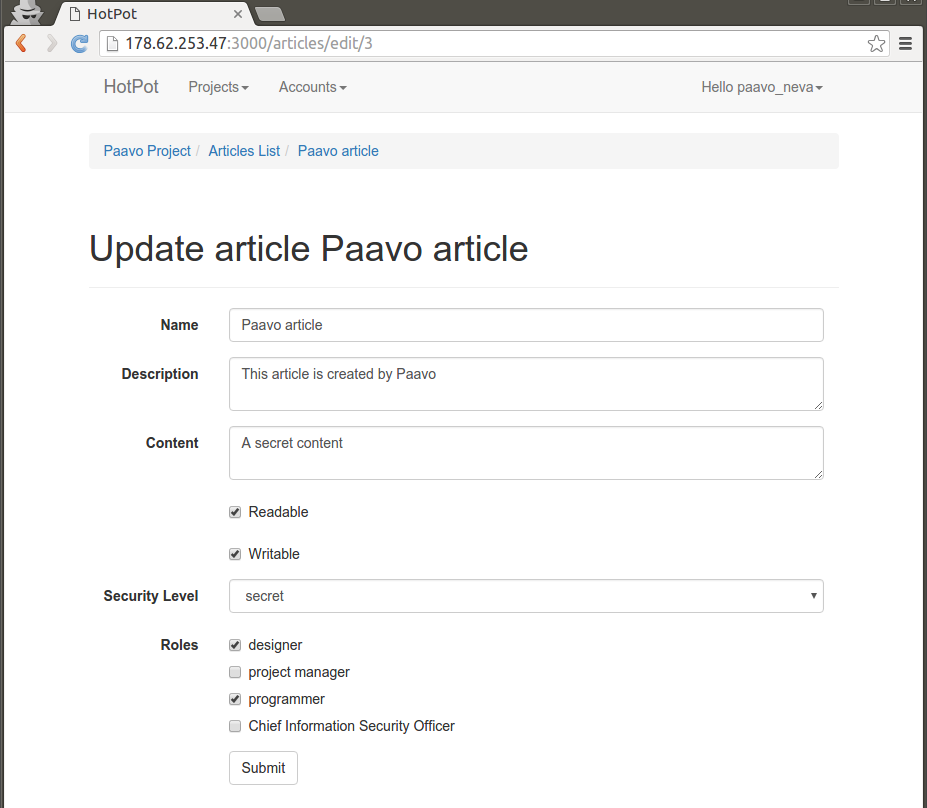
\includegraphics[width=1.0\linewidth]{gfx/chapter_5/article/article_edit}
\caption[Article: article view page]{Article: article edit page}
\label{fig:user_guide:article:article_edit}
\end{figure}

\subsubsection{Delete}
\label{ch:result:user_guide:article:delete}

\begin{description}
\item[Description] Only article's owner can delete it.
\item[Pre-conditions] An article is created as \autoref{ch:result:user_guide:article:create}.
The article's owner logged in.
\item[Results] The article will be deleted.
\end{description}

On the article's view page, click on \emph{Delete} button, as shown in \autoref{fig:user_guide:article:article_view}.

\subsubsection{List}
\label{ch:result:user_guide:article:list}

\begin{description}
\item[Description] Only project's members can see the list of articles in that project.
Articles in the list are filtered upon the member's set of security labels, as discussed in \autoref{ch:hopot_project:project_components}.
\item[Pre-conditions] Project's member logged in.
\item[Results] List of filtered articles.
\end{description}

On the project's view page, click on \emph{Articles} link, then click on \emph{Articles list}, as shown in \autoref{fig:user_guide:article:article_list_link}, to go to \href{http://178.62.253.47:3000/articles/project/3}{http://178.62.253.47:3000/articles/project/3} as shown in \autoref{fig:user_guide:article:article_list}.

\begin{figure}[bth]
\myfloatalign
\subfloat[Article: articles list link]
{
\label{fig:user_guide:article:article_list_link}
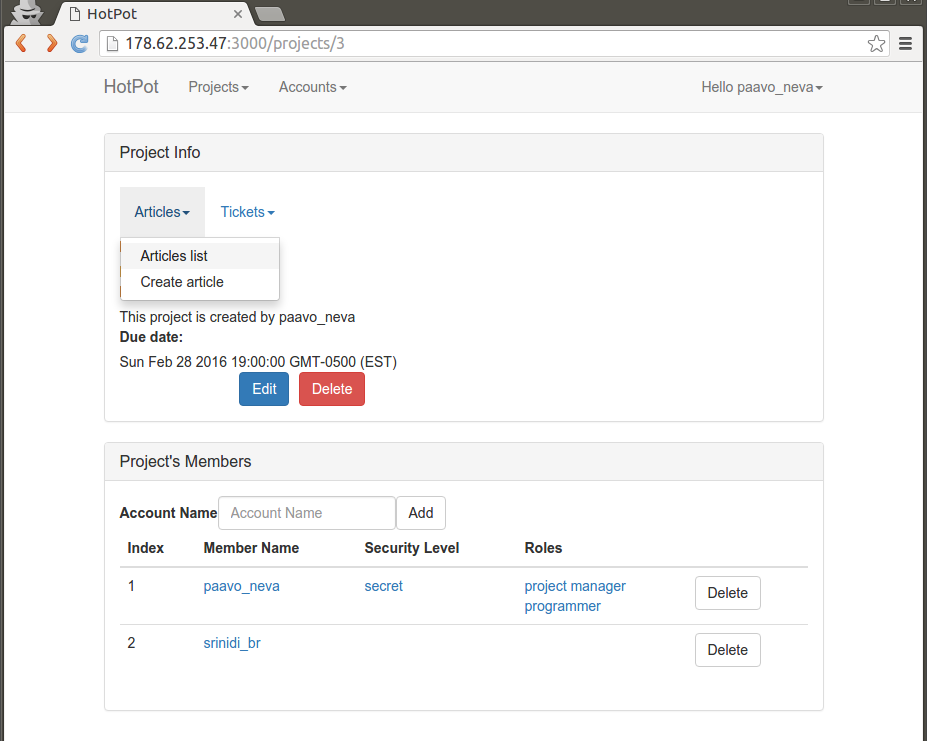
\includegraphics[width=1.\linewidth]{gfx/chapter_5/article/article_list_link}
} \quad
\subfloat[Article: articles list page]
{
\label{fig:user_guide:article:article_list}
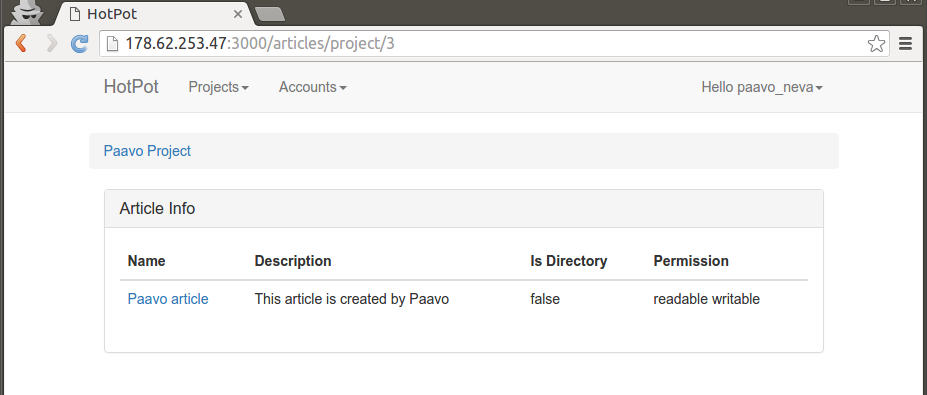
\includegraphics[width=1.\linewidth]{gfx/chapter_5/article/article_list}
} \\
\caption[Article: articles list]{Article: articles list}
\label{fig:user_guide:article:article_list}
\end{figure}

\clearpage

\subsubsection{View}
\label{ch:result:user_guide:article:list}

\begin{description}
\item[Description] Only project's members can view article's details in that project.
Furthemore, the member must either be the article's owner or have a set of security policies which satisfies the article's one.
The access control logics were discussed in \autoref{ch:hopot_project:project_components}.
\item[Pre-conditions] Project's member logged in.
\item[Results] View the article's details.
If the account is permitted, he can view the article as \autoref{fig:user_guide:article:article_view}.
Otherwise, he will redirected to \autoref{fig:user_guide:not_permitted}.
\end{description}

% Ticket guide ----------------------------
\subsection{Ticket}
\label{ch:result:user_guide:ticket}
\subsubsection{Create}
\label{ch:result:user_guide:ticket:create}

\begin{description}
\item[Description] Only project members can create the project's new tickets.
\item[Pre-conditions] Project's member logged in, \eg account \emph{paavo\_neva} and project \emph{Paavo Project}.
\item[Conditions] The ticket's \emph{security level} can only be equal or higher than its creator's.
\item[Parameters] Create new ticket with these values:
\begin{itemize}
\item \emph{name}: Paavo ticket.
\item \emph{content}: A secret content.
\item \emph{due date}: 02/29/2016.
\item \emph{writable}: true.
\item \emph{readable}: true.
\item \emph{priority}: normal.
\item \emph{security level}: secret (equals to account \emph{paavo\_neva}).
\item \emph{role}: designer and programmer.
\end{itemize}
\item[Results] A new ticket will be created under the project.
\end{description}

On the project's view page, click on \emph{Tickets} link, then click on \emph{Create ticket}, as shown in \autoref{fig:user_guide:ticket:ticket_create}, to go to \href{http://178.62.253.47:3000/tickets/create}{http://178.62.253.47:3000/tickets/create}.
Input the ticket's information.
If the inputs are valid, a new ticket will be created and the user will be redirected to the ticket view page as \autoref{fig:user_guide:ticket:ticket_view}.
Otherwise, error messages will be displayed as \autoref{fig:user_guide:ticket:ticket_create_failed}

\begin{figure}[bth]
\myfloatalign
\subfloat[Ticket: tickets create link]
{
\label{fig:user_guide:ticket:ticket_create_link}
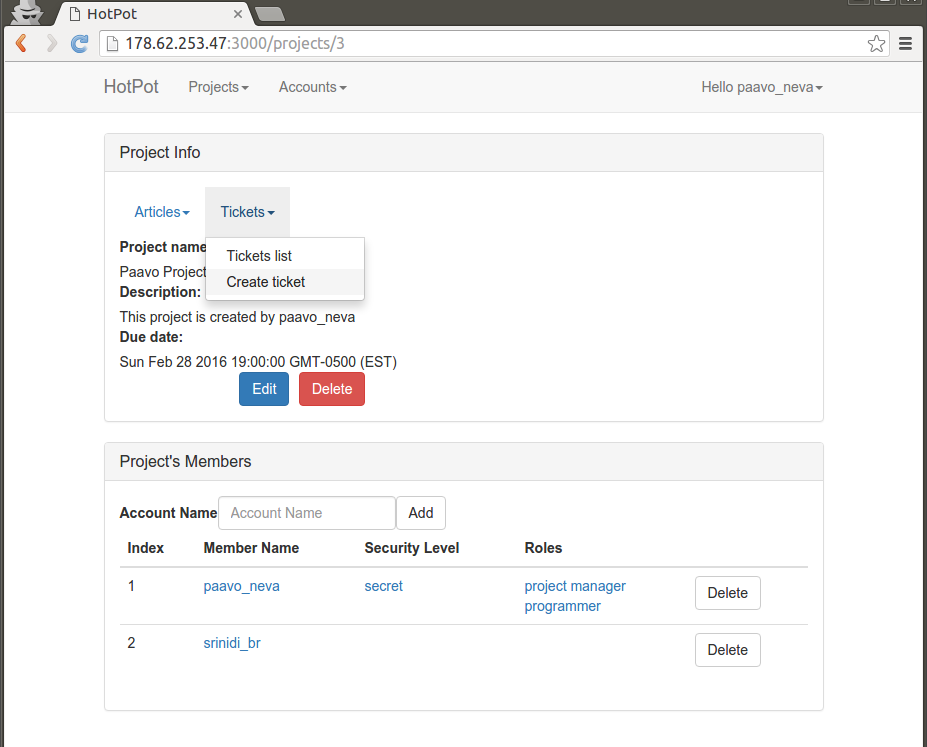
\includegraphics[width=1.\linewidth]{gfx/chapter_5/ticket/ticket_create_link}
} \quad
\subfloat[Ticket: tickets create page]
{
\label{fig:user_guide:ticket:ticket_create}
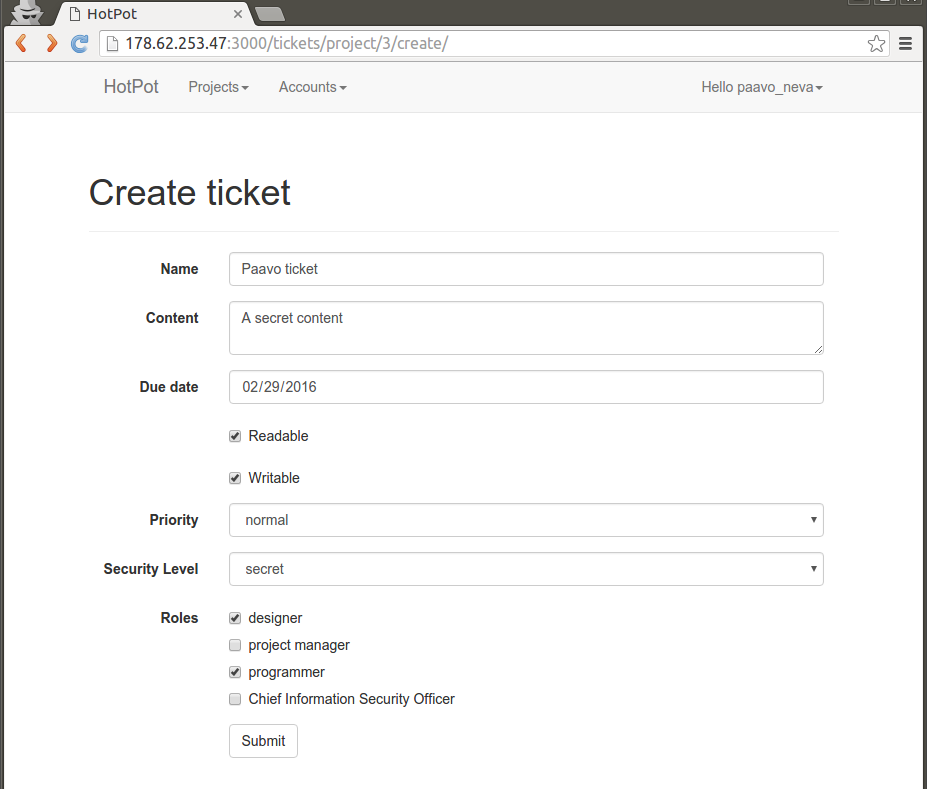
\includegraphics[width=1.\linewidth]{gfx/chapter_5/ticket/ticket_create}
} \\
\caption[Ticket: create tickets]{Ticket: create tickets}
\label{fig:user_guide:ticket:ticket_create}
\end{figure}

\begin{figure}[bth]
\myfloatalign
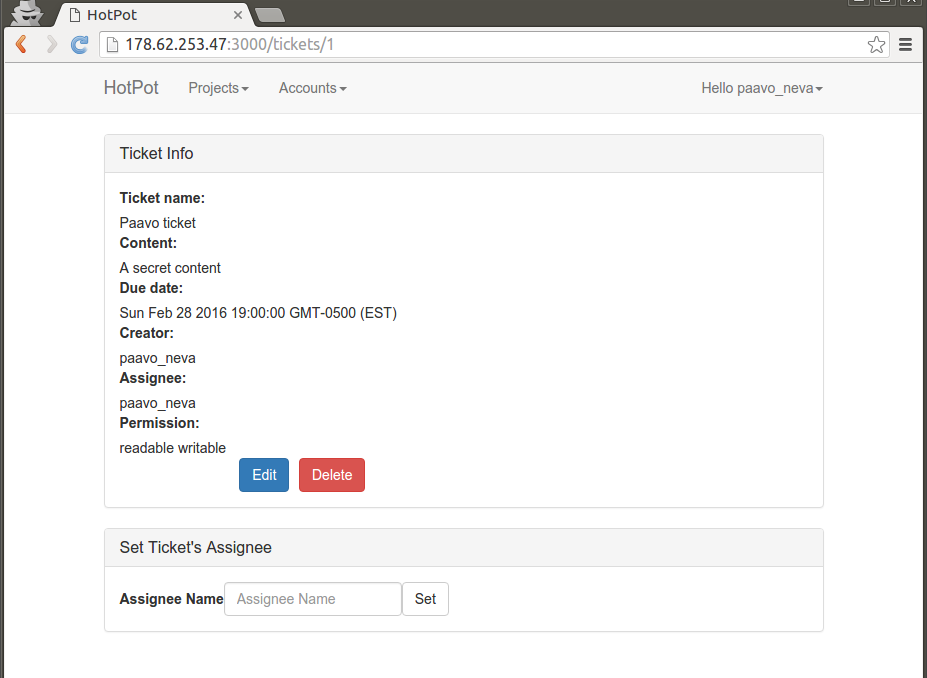
\includegraphics[width=1.0\linewidth]{gfx/chapter_5/ticket/ticket_view}
\caption[Ticket: ticket view page]{Ticket: ticket view page}
\label{fig:user_guide:ticket:ticket_view}
\end{figure}

\begin{figure}[bth]
\myfloatalign
\includegraphics[width=1.0\linewidth]{gfx/chapter_5/ticket/ticket_create_failed}
\caption[Ticket: ticket create failed]{Ticket: ticket creating failed}
\label{fig:user_guide:ticket:ticket_create_failed}
\end{figure}

\clearpage

\subsubsection{Update}
\label{ch:result:user_guide:ticket:update}

\begin{description}
\item[Description] Only project members can update the project's tickets.
Furthemore, the member must either be the ticket's owner or have a set of security policies which satisfies the ticket's one.
The access control logics were discussed in \autoref{ch:hopot_project:project_components}.
\item[Pre-conditions] Project's member logged in, an ticket is created as \autoref{ch:result:user_guide:ticket:create}.
\item[Conditions] The ticket's new \emph{security level} can only be equal or higher than its creator's.
\item[Parameters] Update the ticket with these values:
\begin{itemize}
\item \emph{name}: Paavo ticket.
\item \emph{content}: A top secret content.
\item \emph{due date}: 02/29/2016.
\item \emph{writable}: true.
\item \emph{readable}: true.
\item \emph{priority}: high.
\item \emph{security level}: top secret (equals to account \emph{paavo\_neva}).
\item \emph{role}: programmer.
\end{itemize}
\item[Results] If the input values are valid, the ticket will be updated accordingly.
\end{description}

On the ticket's view page, click on \emph{Edit} button, as shown in \autoref{fig:user_guide:ticket:ticket_view}, to go to \href{http://178.62.253.47:3000/tickets/edit/1}{http://178.62.253.47:3000/tickets/edit/1} as shown in \autoref{fig:user_guide:ticket:ticket_edit}.
Input the ticket's new details.
If the inputs are valid, the ticket will be updated and the user will be redirected to the ticket view page as \autoref{fig:user_guide:ticket:ticket_view}.
Otherwise, error messages will be displayed.

\begin{figure}[bth]
\myfloatalign
\includegraphics[width=1.0\linewidth]{gfx/chapter_5/ticket/ticket_edit}
\caption[Ticket: ticket view page]{Ticket: ticket edit page}
\label{fig:user_guide:ticket:ticket_edit}
\end{figure}

\subsubsection{Delete}
\label{ch:result:user_guide:ticket:delete}

\begin{description}
\item[Description] Only ticket's owner can delete it.
\item[Pre-conditions] An ticket is created as \autoref{ch:result:user_guide:ticket:create}.
The ticket's owner logged in.
\item[Results] The ticket will be deleted.
\end{description}

On the ticket's view page, click on \emph{Delete} button, as shown in \autoref{fig:user_guide:ticket:ticket_view}.

\subsubsection{List}
\label{ch:result:user_guide:ticket:list}

\begin{description}
\item[Description] Only project's members can see the list of tickets in that project.
tickets in the list are filtered upon the member's set of security labels, as discussed in \autoref{ch:hopot_project:project_components}.
\item[Pre-conditions] Project's member logged in.
\item[Results] List of filtered tickets.
\end{description}

On the project's view page, click on \emph{Tickets} link, then click on \emph{Tickets list}, as shown in \autoref{fig:user_guide:ticket:ticket_list_link}, to go to \href{http://178.62.253.47:3000/tickets/project/3}{http://178.62.253.47:3000/tickets/project/3} as shown in \autoref{fig:user_guide:ticket:ticket_list}.

\begin{figure}[bth]
\myfloatalign
\subfloat[Ticket: tickets list link]
{
\label{fig:user_guide:ticket:ticket_list_link}
\includegraphics[width=1.\linewidth]{gfx/chapter_5/ticket/ticket_list_link}
} \quad
\subfloat[Ticket: tickets list page]
{
\label{fig:user_guide:ticket:ticket_list}
\includegraphics[width=1.\linewidth]{gfx/chapter_5/ticket/ticket_list}
} \\
\caption[Ticket: tickets list]{Ticket: tickets list}
\label{fig:user_guide:ticket:ticket_list}
\end{figure}

\clearpage

\subsubsection{View}
\label{ch:result:user_guide:ticket:list}

\begin{description}
\item[Description] Only project's members can view ticket's details in that project.
Furthemore, the member must either be the ticket's owner or have a set of security policies which satisfies the ticket's one.
The access control logics were discussed in \autoref{ch:hopot_project:project_components}.
\item[Pre-conditions] Project's member logged in.
\item[Results] View the ticket's details.
If the account is permitted, he can view the ticket as \autoref{fig:user_guide:ticket:ticket_view}.
Otherwise, he will redirected to \autoref{fig:user_guide:not_permitted}.
\end{description}

\subsubsection{Assign member}
\label{ch:result:user_guide:ticket:managing_member}

\begin{description}
\item[Description] Every project's members can assign ticket to another member.
Furthermore, this action is considered similar to \emph{edit}, so that it also need to follow \emph{edit}'s policies.
\item[Pre-conditions] A project member logged in, \eg account \emph{paavo\_neva}.
\item[Parameters] Set user \emph{khangnguyen} as the ticket's assignee.
\item[Results] The account will be set as the ticket's assignee.
\end{description}

After logging in as the project's member, go to a ticket in URL \href{http://178.62.253.47:3000/tickets/1}{http://178.62.253.47:3000/tickets/1}.
Input the \emph{account's name} and the result will be shown as \autoref{fig:user_guide:ticket:ticket_assign}.

\begin{figure}[bth]
\myfloatalign
\subfloat[Ticket: inputting ticket's assignee username]
{
\label{fig:user_guide:ticket:input_new_member}
\includegraphics[width=1.\linewidth]{gfx/chapter_5/ticket/ticket_assign}
} \quad
\subfloat[Ticket: assigning ticket's assignee successfully]
{
\label{fig:user_guide:ticket:ticket_view}
\includegraphics[width=1.\linewidth]{gfx/chapter_5/ticket/ticket_assign_successfully}
} \\
\caption[Ticket: assigning ticket's assignee]{Ticket: assigning ticket's assignee}
\label{fig:user_guide:ticket:ticket_assign}
\end{figure}

\clearpage

% Security Level guide ----------------------------
\subsection{Security Level}
\label{ch:result:user_guide:security_level}
\subsubsection{Create}
\label{ch:result:user_guide:security_level:create}

\begin{description}
\item[Description] Only administrators can create the system's new security level.
\item[Pre-conditions] A logged in administrator account, \eg account \emph{khangnguyen:khangnguyen}.
\item[Parameters] Create new security level with these values:
\begin{itemize}
\item \emph{name}: God file.
\item \emph{level}: 5 (the higher level the more secured the label is).
\item \emph{description}: Ultimately secret level.
\end{itemize}
\item[Results] A new security level label will be created in the system.
\end{description}

On admin interface, on the top bar, click on \emph{Security Levels} link, then click on \emph{Create level}, as shown in \autoref{fig:user_guide:security_level:level_links}, 
to go to \href{http://178.62.253.47:3000/security\_levels/create}{http://178.62.253.47:3000/security\_levels/create} as shown in \autoref{fig:user_guide:security_level:level_create}.
Input the security level's information.
If the inputs are valid, a new security level will be created and the administrator will be redirected to the security level view page as \autoref{fig:user_guide:security_level:level_view}.
Otherwise, error messages will be displayed as \autoref{fig:user_guide:security_level:level_create_failed}

\begin{figure}[bth]
\myfloatalign
\subfloat[Security Level: security level create link]
{
\label{fig:user_guide:security_level:level_links}
\includegraphics[width=1.\linewidth]{gfx/chapter_5/security_level/level_links}
} \quad
\subfloat[Security Level: security level create page]
{
\label{fig:user_guide:security_level:security_level_create}
\includegraphics[width=1.\linewidth]{gfx/chapter_5/security_level/level_create}
} \\
\caption[Security Level: create security level]{Security Level: create security level}
\label{fig:user_guide:security_level:level_create}
\end{figure}

\begin{figure}[bth]
\myfloatalign
\includegraphics[width=1.0\linewidth]{gfx/chapter_5/security_level/level_view}
\caption[Security Level: security level view page]{Security Level: security level view page}
\label{fig:user_guide:security_level:level_view}
\end{figure}

\begin{figure}[bth]
\myfloatalign
\includegraphics[width=1.0\linewidth]{gfx/chapter_5/security_level/level_create_failed}
\caption[Security Level: security level create]{Security Level: security level creating failed}
\label{fig:user_guide:security_level:level_create_failed}
\end{figure}

\clearpage

\subsubsection{Update}
\label{ch:result:user_guide:security_level:update}

\begin{description}
\item[Description] Only administrators can update the system's existing security levels.
\item[Pre-conditions] A logged in administrator account, \eg account \emph{khangnguyen:khangnguyen}.
A security level is created as \autoref{ch:result:user_guide:security_level:create}
\item[Parameters] Update the security level with these values:
\begin{itemize}
\item \emph{name}: Sheep file.
\item \emph{level}: 1.
\item \emph{description}: Ultimately low level.
\end{itemize}
\item[Results] The level will be updated.
\end{description}

On the security level's view page, click on \emph{Edit} button, as shown in \autoref{fig:user_guide:security_level:level_view}, 
to go to \href{http://178.62.253.47:3000/security\_levels/edit/6}{http://178.62.253.47:3000/security\_levels/edit/6} as shown in \autoref{fig:user_guide:security_level:level_edit}.
Input the security level's new details.
If the inputs are valid, the security level will be updated and the administrator will be redirected to the security level view page as \autoref{fig:user_guide:security_level:level_view}.
Otherwise, error messages will be displayed.

\begin{figure}[bth]
\myfloatalign
\includegraphics[width=1.0\linewidth]{gfx/chapter_5/security_level/level_edit}
\caption[Security Level: security level edit page]{Security Level: security level edit page}
\label{fig:user_guide:security_level:level_edit}
\end{figure}

\subsubsection{Delete}
\label{ch:result:user_guide:security_level:delete}

\begin{description}
\item[Description] Only administrators can delete the system's existing security levels.
\item[Pre-conditions] A logged in administrator account, \eg account \emph{khangnguyen:khangnguyen}.
A security level is created as \autoref{ch:result:user_guide:security_level:create}
\item[Results] The level will be deleted.
\end{description}

On the security level's view page, click on \emph{Delete} button, as shown in \autoref{fig:user_guide:security_level:level_view}.

\subsubsection{List and View}
\label{ch:result:user_guide:security_level:list}

\begin{description}
\item[Description] Every accounts can view the list of security levels in the system, as well as their details.
\item[Pre-conditions] A logged in account, \eg account \emph{khangnguyen:khangnguyen}.
\item[Results] The list of security levels is shown.
\end{description}

On admin interface, on the top bar, click on \emph{Security Levels} link, then click on \emph{Levels list}, as shown in \autoref{fig:user_guide:security_level:level_links}, 
to go to \href{http://178.62.253.47:3000/security\_levels}{http://178.62.253.47:3000/security\_levels} as shown in \autoref{fig:user_guide:security_level:level_list}.

\begin{figure}[bth]
\myfloatalign
\includegraphics[width=1.0\linewidth]{gfx/chapter_5/security_level/level_list}
\caption[Security Level: security level list page]{Security Level: security level list page}
\label{fig:user_guide:security_level:level_list}
\end{figure}

% Role guide ----------------------------
\subsection{Role}
\label{ch:result:user_guide:role}
\subsubsection{Create}
\label{ch:result:user_guide:role:create}

\begin{description}
\item[Description] Only administrators can create the system's new role.
\item[Pre-conditions] A logged in administrator account, \eg account \emph{khangnguyen:khangnguyen}.
\item[Parameters] Create new role with these values:
\begin{itemize}
\item \emph{name}: System admin.
\item \emph{description}: He fix your machine.
\end{itemize}
\item[Results] A new role label will be created in the system.
\end{description}

On admin interface, on the top bar, click on \emph{Roles} link, then click on \emph{Create role}, as shown in \autoref{fig:user_guide:role:role_links}, 
to go to \href{http://178.62.253.47:3000/roles/create}{http://178.62.253.47:3000/roles/create} as shown in \autoref{fig:user_guide:role:role_create}.
Input the role's information.
If the inputs are valid, a new role will be created and the administrator will be redirected to the role view page as \autoref{fig:user_guide:role:role_view}.
Otherwise, error messages will be displayed as \autoref{fig:user_guide:role:role_create_failed}

\begin{figure}[bth]
\myfloatalign
\subfloat[Role: role create link]
{
\label{fig:user_guide:role:role_links}
\includegraphics[width=1.\linewidth]{gfx/chapter_5/role/role_links}
} \quad
\subfloat[Role: role create page]
{
\label{fig:user_guide:role:role_create}
\includegraphics[width=1.\linewidth]{gfx/chapter_5/role/role_create}
} \\
\caption[Role: create role]{Role: create role}
\label{fig:user_guide:role:role_create}
\end{figure}

\begin{figure}[bth]
\myfloatalign
\includegraphics[width=1.0\linewidth]{gfx/chapter_5/role/role_view}
\caption[Role: role view page]{Role: role view page}
\label{fig:user_guide:role:role_view}
\end{figure}

\begin{figure}[bth]
\myfloatalign
\includegraphics[width=1.0\linewidth]{gfx/chapter_5/role/role_create_failed}
\caption[Role: role create]{Role: role creating failed}
\label{fig:user_guide:role:role_create_failed}
\end{figure}

\clearpage

\subsubsection{Update}
\label{ch:result:user_guide:role:update}

\begin{description}
\item[Description] Only administrators can update the system's existing roles.
\item[Pre-conditions] A logged in administrator account, \eg account \emph{khangnguyen:khangnguyen}.
A role is created as \autoref{ch:result:user_guide:role:create}
\item[Parameters] Update the role with these values:
\begin{itemize}
\item \emph{name}: System admin.
\item \emph{description}: He fix your machine, and back you up.
\end{itemize}
\item[Results] The role will be updated.
\end{description}

On the role's view page, click on \emph{Edit} button, as shown in \autoref{fig:user_guide:role:role_view}, 
to go to \href{http://178.62.253.47:3000/roles/edit/6}{http://178.62.253.47:3000/roles/edit/6} as shown in \autoref{fig:user_guide:role:role_edit}.
Input the role's new details.
If the inputs are valid, the role will be updated and the administrator will be redirected to the role view page as \autoref{fig:user_guide:role:role_view}.
Otherwise, error messages will be displayed.

\begin{figure}[bth]
\myfloatalign
\includegraphics[width=1.0\linewidth]{gfx/chapter_5/role/role_edit}
\caption[Role: role edit page]{Role: role edit page}
\label{fig:user_guide:role:role_edit}
\end{figure}

\subsubsection{Delete}
\label{ch:result:user_guide:role:delete}

\begin{description}
\item[Description] Only administrators can delete the system's existing roles.
\item[Pre-conditions] A logged in administrator account, \eg account \emph{khangnguyen:khangnguyen}.
A role is created as \autoref{ch:result:user_guide:role:create}
\item[Results] The role will be deleted.
\end{description}

On the role's view page, click on \emph{Delete} button, as shown in \autoref{fig:user_guide:role:role_view}.

\subsubsection{List and View}
\label{ch:result:user_guide:role:list}

\begin{description}
\item[Description] Every accounts can view the list of roles in the system, as well as their details.
\item[Pre-conditions] A logged in account, \eg account \emph{khangnguyen:khangnguyen}.
\item[Results] The list of roles is shown.
\end{description}

On admin interface, on the top bar, click on \emph{Roles} link, then click on \emph{roles list}, as shown in \autoref{fig:user_guide:role:role_links}, 
to go to \href{http://178.62.253.47:3000/roles}{http://178.62.253.47:3000/roles} as shown in \autoref{fig:user_guide:role:role_list}.

\begin{figure}[bth]
\myfloatalign
\includegraphics[width=1.0\linewidth]{gfx/chapter_5/role/role_list}
\caption[Role: role list page]{Role: role list page}
\label{fig:user_guide:role:role_list}
\end{figure}

% Priority guide ----------------------------
\subsection{Priority}
\label{ch:result:user_guide:priority}
\subsubsection{Create}
\label{ch:result:user_guide:priority:create}

\begin{description}
\item[Description] Only administrators can create the system's new priority.
\item[Pre-conditions] A logged in administrator account, \eg account \emph{khangnguyen:khangnguyen}.
\item[Parameters] Create new priority with these values:
\begin{itemize}
\item \emph{name}: Highest Priority.
\item \emph{level}: 5 (the higher level the higher the priority is).
\item \emph{description}: Ultimately high priority.
\end{itemize}
\item[Results] A new priority label will be created in the system.
\end{description}

On admin interface, on the top bar, click on \emph{Priorities} link, then click on \emph{Create priority}, as shown in \autoref{fig:user_guide:priority:priority_links}, 
to go to \href{http://178.62.253.47:3000/priorities/create}{http://178.62.253.47:3000/priorities/create} as shown in \autoref{fig:user_guide:priority:priority_create}.
Input the priority's information.
If the inputs are valid, a new priority will be created and the administrator will be redirected to the priority view page as \autoref{fig:user_guide:priority:priority_view}.
Otherwise, error messages will be displayed as \autoref{fig:user_guide:priority:priority_create_failed}

\begin{figure}[bth]
\myfloatalign
\subfloat[Priority: priority create link]
{
\label{fig:user_guide:priority:priority_links}
\includegraphics[width=1.\linewidth]{gfx/chapter_5/priority/priority_links}
} \quad
\subfloat[Priority: priority create page]
{
\label{fig:user_guide:priority:priority_create}
\includegraphics[width=1.\linewidth]{gfx/chapter_5/priority/priority_create}
} \\
\caption[Priority: create priority]{priority: create priority}
\label{fig:user_guide:priority:priority_create}
\end{figure}

\begin{figure}[bth]
\myfloatalign
\includegraphics[width=1.0\linewidth]{gfx/chapter_5/priority/priority_view}
\caption[priority: priority view page]{priority: priority view page}
\label{fig:user_guide:priority:priority_view}
\end{figure}

\begin{figure}[bth]
\myfloatalign
\includegraphics[width=1.0\linewidth]{gfx/chapter_5/priority/priority_create_failed}
\caption[priority: priority create]{priority: priority creating failed}
\label{fig:user_guide:priority:priority_create_failed}
\end{figure}

\clearpage

\subsubsection{Update}
\label{ch:result:user_guide:priority:update}

\begin{description}
\item[Description] Only administrators can update the system's existing priorities.
\item[Pre-conditions] A logged in administrator account, \eg account \emph{khangnguyen:khangnguyen}.
A priority is created as \autoref{ch:result:user_guide:priority:create}
\item[Parameters] Update the priority with these values:
\begin{itemize}
\item \emph{name}: Sheep file.
\item \emph{level}: 1.
\item \emph{description}: Ultimately low priority.
\end{itemize}
\item[Results] The priority will be updated.
\end{description}

On the priority's view page, click on \emph{Edit} button, as shown in \autoref{fig:user_guide:priority:priority_view}, 
to go to \href{http://178.62.253.47:3000/priorities/edit/6}{http://178.62.253.47:3000/priorities/edit/6} as shown in \autoref{fig:user_guide:priority:priority_edit}.
Input the priority's new details.
If the inputs are valid, the priority will be updated and the administrator will be redirected to the priority view page as \autoref{fig:user_guide:priority:priority_view}.
Otherwise, error messages will be displayed.

\begin{figure}[bth]
\myfloatalign
\includegraphics[width=1.0\linewidth]{gfx/chapter_5/priority/priority_edit}
\caption[Priority: priority edit page]{Priority: priority edit page}
\label{fig:user_guide:priority:priority_edit}
\end{figure}

\subsubsection{Delete}
\label{ch:result:user_guide:priority:delete}

\begin{description}
\item[Description] Only administrators can delete the system's existing priorities.
\item[Pre-conditions] A logged in administrator account, \eg account \emph{khangnguyen:khangnguyen}.
A priority is created as \autoref{ch:result:user_guide:priority:create}
\item[Results] The priority will be deleted.
\end{description}

On the priority's view page, click on \emph{Delete} button, as shown in \autoref{fig:user_guide:priority:priority_view}.

\subsubsection{List and View}
\label{ch:result:user_guide:priority:list}

\begin{description}
\item[Description] Every accounts can view the list of priorities in the system, as well as their details.
\item[Pre-conditions] A logged in account, \eg account \emph{khangnguyen:khangnguyen}.
\item[Results] The list of priorities is shown.
\end{description}

On admin interface, on the top bar, click on \emph{Priorities} link, then click on \emph{priorities list}, as shown in \autoref{fig:user_guide:priority:priority_links}, 
to go to \href{http://178.62.253.47:3000/priorities}{http://178.62.253.47:3000/priorities} as shown in \autoref{fig:user_guide:priority:priority_list}.

\begin{figure}[bth]
\myfloatalign
\includegraphics[width=1.0\linewidth]{gfx/chapter_5/priority/priority_list}
\caption[Priority: priority list page]{Priority: priority list page}
\label{fig:user_guide:priority:priority_list}
\end{figure}

%----------------------------------------------------------------------------------------
\section{Learnings}

As working on the project, I have learned many new things.
First of all, technically, this is my second \emph{Nodejs} project.
So in this project, I deliberately chose it for study purpose.
After the project, I had an improving about \emph{Nodejs} and one of its most popular framework \emph{Expressjs}.
All of my experiences and learning about it are noted in \emph{diary} directory on GitHub repository which is listed in \autoref{ch:appendix:repository_structure}.
Those diaries are my daily reports of what I have done, the problems occurred on that day, and their solutions if available\dots

About programming experience, there is one advise which may be very useful when we have to due with unfamiliar issues of new technologies: always spend time for reading the technology's documents.
\marginpar{``Give me six hours to chop down a tree and I will spend the first four sharpening the axe'' -- Abraham Lincoln (1809-1865) }
Obviously, with the strong supports of huge technical communities these days, we can easily finish our jobs by searching for available solutions.
However, it does not help us to master the technology on our own \ie we don't understand it enough to handle other problems in the future.
Reading documentation will profit us in understand the technology's principles, from that we can study best practices in using it.
Consequently, it will improve our performance in using it.
On the other hand, spending time on learning a technology properly, we will also learn its owner's experience on programming and problems solving skills.
In another word, we can inherit his programming mindsets, design patterns which could be profitable in our future projects.
My suggestion is to put technology studying as a task in the project's tasks list, and assign a time span to it as an usual one.
The time span should be long enough for reading through the technology's documents, and not too long or it will become time consuming.
It took me two days to learn about \emph{Expressjs} enough for me to start working with it initially.
And it takes the same amount of time for me to studying using some crucial libraries such as \emph{Sequelizejs}, \emph{Promise}\dots
And on the working progress, I can learn more about their good practices.

Besides that, studying about MLS is a huge advantage to me.
Security is always a hot and essential topic, MLS is one of it.
Through the project, I learned about the MLS policies, and how they could be implemented in a system.
We have to design a blueprint of the system based on selected MLS model.
The blueprint consists of rules that \emph{subjects} and \emph{objects} of the system must be devoted to.
In the progress, we need to review it multiple times in multiple points of view to ensure that there is no exception.
Rather than that, again, there is no \emph{one master solution for all problems}, sometimes we have to make compromises.
In another word, for example, we have to make trade-off between performance and security.
The high secured system may be complicated and inflexible; however, flexible system with many \emph{trusted subjects/objects} could pose security leaks in the future.
So that, whenever we have to make a compromise, we have to acknowledge and keep in mind (or better, in note) its consequences to avoid in future work.

Planing is also an extensive skill.
Although, this project is my personal project, I learned a lot of time management.
In my own opinion, at the first try, we should assign a task with a small extension of time than we have evaluated.
We should not give a too tight time slot for very first tasks, there will be usually some modifications in features list and project requirements at the first stage of the project; and making early decisions very likely leads to changes.
As the progress goes on, the project is also getting stable.
The number of sudden changes or making decision will decrease remarkably.
Consequently, at this time, we can shorten the addition time extension, or just omit it.

 % Chapter 5

%----------------------------------------------------------------------------------------
%	THESIS CONTENT - APPENDICES
%----------------------------------------------------------------------------------------

%\appendix

%\part{Appendix} % New part of the thesis for the appendix

%% Appendix A

\chapter{Appendices}
\label{ch:appendix-a}

%----------------------------------------------------------------------------------------

\section{Installation Guide}
\label{ch:appendix-a:installation_guide}

\autoref{ch:implementation:technical_information} listed the technical requirements for this project.
In this guide, we will learn about the project's setup from scratch, step by step.

Assume that you already have a machine running CentOS 7 with these packages have already been installed: \emph{git, postgresql, nodejs with npm}.
I am using \emph{Digital Ocean} as VPS provider.
I create a \emph{Digital Ocean's droplet} with this specification: \emph{512MB Ram 20GB SSD Disk CentOS 7.1 x64}.
A postgresql database should be created and named as \emph{hotpot} whose owner is \emph{hotpot} and the password at your own choice.

First of all we need to clone the project's source code from GitHub using the command.
\begin{lstlisting}[breaklines=false,frame=lt]
$ git clone git@github.com:khangpn/hotpot.git
\end{lstlisting}

Next, we need to install all the project's dependencies by going into the project's root directory and execute \emph{npm} install command
\begin{lstlisting}[breaklines=false,frame=lt]
$/hotpot/ npm install
\end{lstlisting}
This command may take a while to install all required packages.

After checking the database accessibility, we need to configure its connection in \emph{config\/database.js}. 
Open that file by your favorite text editor, my choice is \emph{vim}. 
\begin{lstlisting}[breaklines=false,frame=lt]
$/hotpot/ vim config/database.js
\end{lstlisting}

Below is an example of the database configuration, if the database name, its user and password are \emph{hotpot} and the database is running on local machine, then your configuration file should be similar to this.
\begin{lstlisting}[breaklines=false,frame=lt]
var settings = {                                                                                                                                                     
  development: { 
    database : "hotpot",
    username : "hotpot",
    password : "hotpot",
    options  : { 
      dialect : "postgresql",
      host     : "127.0.0.1"   
    }
  },
  production: { 
    database : "hotpot",
    username : "hotpot",
    password : "hotpot",
    options  : { 
      dialect : "postgresql",  
      host     : "127.0.0.1"   
    }
  }
};
  
module.exports = settings;
\end{lstlisting}

Next, lets open file \emph{setup} and change its \emph{NODE\_ENV} to \emph{development} or \emph{production} depending on your purpose.
\emph{Development} environemnt will print out the system's logs on our server and return errors' full stack trace to client, while  \emph{production} will omit it.
\begin{lstlisting}[breaklines=false,frame=lt]
// file hotpot/setup
NODE_ENV=development DEBUG=hotpot node bin/db-integration.js
\end{lstlisting}

Also edit file \emph{start} to change its \emph{NODE\_ENV}
\begin{lstlisting}[breaklines=false,frame=lt]
// file hotpot/start
NODE_ENV=development DEBUG=hotpot npm start
\end{lstlisting}
We can also add \emph{PORT} variable to the script to specify the project's running port. By default, it runs on port \emph{3000}
\begin{lstlisting}[breaklines=false,frame=lt]
// file hotpot/start
NODE_ENV=development PORT=4000 DEBUG=hotpot npm start
\end{lstlisting}

Next, we have to initialize the project's database schema using the \emph{setup} script.
\begin{lstlisting}[breaklines=false,frame=lt]
$/hotpot/ ./setup
\end{lstlisting}
This setup may take a while. And finally we can start the project using the \emph{start} script.
\begin{lstlisting}[breaklines=false,frame=lt]
$/hotpot/ ./start
\end{lstlisting}

%----------------------------------------------------------------------------------------

\section{Manual}
\label{ch:appendix-a:user_guide}

As the demonstration for this project, I have deployed \myProject at the address \href{http://178.62.253.47:3000/}{http://178.62.253.47:3000/}.
In this section, we are going through demonstrations of the project's features \ie test cases of the project's behaviours.

% Miscellaneous guide ----------------------------
\subsection{Miscellaneous}
\label{ch:appendix-a:user_guide:miscellaneous}
\autoref{fig:user_guide:homepage}, \autoref{fig:user_guide:user_interface}, \autoref{fig:user_guide:admin_interface},\autoref{fig:user_guide:profile}, and \autoref{fig:user_guide:not_permitted} are some general interfaces which are visible across the guide.

\begin{figure}[bth]                                                                                                                                                  \myfloatalign
\includegraphics[width=1.0\linewidth]{gfx/chapter_5/general/homepage}
\caption[HotPot homepage]{HotPot homepage}
\label{fig:user_guide:homepage}
\end{figure}

\begin{figure}[bth]                                                                                                                                                  \myfloatalign
\includegraphics[width=1.0\linewidth]{gfx/chapter_5/general/user_interface}
\caption[HotPot user interface]{HotPot user interface}
\label{fig:user_guide:user_interface}
\end{figure}

\begin{figure}[bth]                                                                                                                                                  \myfloatalign
\includegraphics[width=1.0\linewidth]{gfx/chapter_5/general/admin_interface}
\caption[HotPot admin interface]{HotPot admin interface}
\label{fig:user_guide:admin_interface}
\end{figure}

\begin{figure}[bth]                                                                                                                                                  \myfloatalign
\includegraphics[width=1.0\linewidth]{gfx/chapter_5/general/profile}
\caption[HotPot profile page]{HotPot profile page}
\label{fig:user_guide:profile}
\end{figure}

\begin{figure}[bth]                                                                                                                                                  \myfloatalign
\includegraphics[width=1.0\linewidth]{gfx/chapter_5/general/not_permitted}
\caption[HotPot not permitted error]{HotPot not permitted error}
\label{fig:user_guide:not_permitted}
\end{figure}

\clearpage

\subsubsection{Login}
\label{ch:appendix-a:user_guide:miscellaneous:login}

\begin{description}
\item[Description] Every accounts can login to the system using its username and password.
\item[Parameters] An account whose username:password are:
\begin{itemize}
\item \emph{username}: paavo\_neva.
\item \emph{password}: paavo\_neva.
\end{itemize}
\item[Results] If the account is authenticated then a token is created and save on client cookies, and the user is redirected to homepage.
If the account is invalid, the login page will be rendered with error messages.
\end{description}

On homepage \autoref{fig:user_guide:homepage} click on \emph{Log in} link on the top bar to go to \href{http://178.62.253.47:3000/login}{http://178.62.253.47:3000/login}.

\begin{figure}[bth]                                                                                                                                                  \myfloatalign
\includegraphics[width=1.0\linewidth]{gfx/chapter_5/miscellaneous/login}
\caption[HotPot login page]{HotPot login page}
\label{fig:user_guide:miscellaneous:login}
\end{figure}

\begin{figure}[bth]
\myfloatalign
\subfloat[Login failed]
{
\label{fig:user_guide:miscellaneous:login_failed}
\includegraphics[width=1.\linewidth]{gfx/chapter_5/miscellaneous/login_failed}
} \quad
\subfloat[Login successfully then redirected to profile page]
{
\label{fig:user_guide:miscellaneous:profile}
\includegraphics[width=1.\linewidth]{gfx/chapter_5/general/profile}
} \\
\caption[Login results]{Login results}
\label{fig:user_guide:login:result}
\end{figure}

\clearpage

\subsubsection{Logout}
\label{ch:appendix-a:user_guide:miscellaneous:logout}

\begin{description}
\item[Description] Every logged in accounts can logout from the system.
\item[Parameters] A logged in account.
\item[Results] The account will be logged out.
Its token will be deleted.
All of his cookies data on the client will be emptied.
Finally, he will be redirected to homepage.
\end{description}

After logging in, on any pages, click on the username link to show \emph{Log out} link.
Click on it for logging out.
After that, the user will be redirected to \emph{homepage} \(\autoref{fig:user_guide:homepage}\).

\begin{figure}[bth]                                                                                                                                                  \myfloatalign
\includegraphics[width=1.0\linewidth]{gfx/chapter_5/miscellaneous/logout}
\caption[HotPot logout link]{HotPot logout link}
\label{fig:user_guide:miscellaneous:logout}
\end{figure}

%\clearpage

% Account guide ----------------------------
\subsection{Account}
\label{ch:appendix-a:user_guide:account}
\subsubsection{Create}
\label{ch:appendix-a:user_guide:account:create}

\begin{description}
\item[Description] Administrators can create new accounts on the system.
\item[Pre-conditions] An administrator account is logged in.
\item[Parameters] Create an account with values:
\begin{itemize}
\item \emph{username}: testingtesting.
\item \emph{password}: testingtesting.
\end{itemize}
\item[Results] If all the input information is valid, new account will be created, otherwise error messages will be displayed.
\end{description}

After logging in as an administrator, the user interface will appeared like in \autoref{fig:user_guide:admin_interface}.
On the tool bar, click on \emph{Accounts}, then \emph{Create account}.
The creating page will appear under URL

\noindent\href{http://178.62.253.47:3000/accounts/create}{http://178.62.253.47:3000/accounts/create} as shown in \autoref{fig:user_guide:account:account_create}.
Input the value, the \emph{Confirm Password} field is for re-typing password, and the result will be shown as \autoref{fig:user_guide:account:account_create_result}.

\begin{figure}[bth]
\myfloatalign
\subfloat[HotPot Account creation link]
{
\label{fig:user_guide:account:account_create_link}
\includegraphics[width=1.0\linewidth]{gfx/chapter_5/account/account_create_link}
} \quad
\subfloat[HotPot Account creating page]
{
\label{fig:user_guide:account:account_create}
\includegraphics[width=1.0\linewidth]{gfx/chapter_5/account/account_create}
} \\
\caption[HotPot Account creation]{HotPot Account creating}
\label{fig:user_guide:account:account_create}
\end{figure}

\begin{figure}[bth]
\myfloatalign
\subfloat[Account creating failed]
{
\includegraphics[width=1.\linewidth]{gfx/chapter_5/account/account_create_failed}
} \quad
\subfloat[Account creating successfully then redirected to account detail page]
{
\label{fig:user_guide:account:account_view}
\includegraphics[width=1.\linewidth]{gfx/chapter_5/account/account_view}
} \\
\caption[Login results]{Account creating results}
\label{fig:user_guide:account:account_create_result}
\end{figure}

\clearpage

\subsubsection{Edit profile}
\label{ch:appendix-a:user_guide:account:profile}

\begin{description}
\item[Description] Account's owner can edit his all profile details.
\item[Pre-conditions] An account is logged in.
\item[Parameters] Update the logged in account's profile with values:
\begin{itemize}
\item \emph{fullname}: Paavo Neva.
\item \emph{email}: paavo@hotpot.com.
\end{itemize}
\item[Results] If all the input information is valid, the account's profile will be updated.
\end{description}

After logging in, the user interface will appeared like in \autoref{fig:user_guide:user_interface}.
On the tool bar, click on the account name on left top corner, then \emph{Profile} as shown in \autoref{fig:user_guide:account:profile_link}.
The account's profile page will appear under URL \href{http://178.62.253.47:3000/accounts/3}{http://178.62.253.47:3000/accounts/3} as shown in \autoref{fig:user_guide:profile}.
Click on \emph{Edit Profile} link, to go to 

\noindent\href{http://178.62.253.47:3000/accounts/update\_detail}{http://178.62.253.47:3000/accounts/update\_detail} as shown in 
\autoref{fig:user_guide:account:edit_profile}
Input the value, and the result will be shown as \autoref{fig:user_guide:account:profile_updated}.

\begin{figure}[bth]
\myfloatalign
\subfloat[HotPot Profile update link]
{
\label{fig:user_guide:account:profile_link}
\includegraphics[width=1.0\linewidth]{gfx/chapter_5/account/profile_link}
} \quad
\subfloat[HotPot Profile editing page]
{
\label{fig:user_guide:account:edit_profile}
\includegraphics[width=1.0\linewidth]{gfx/chapter_5/account/edit_profile}
} \\
\caption[HotPot Account creation]{HotPot Account creating}
\label{fig:user_guide:account:edit_profile}
\end{figure}

\begin{figure}[bth]                                                                                                                                                  \myfloatalign
\includegraphics[width=1.0\linewidth]{gfx/chapter_5/account/profile_updated}
\caption[HotPot Profile updated]{HotPot Profile updated}
\label{fig:user_guide:account:profile_updated}
\end{figure}

\subsubsection{Change Password}
\label{ch:appendix-a:user_guide:account:change_password}

\begin{description}
\item[Description] Account's owner can change his password.
\item[Pre-conditions] An account is logged in.
\item[Parameters] Update the logged in account's password with values:
\begin{itemize}
\item \emph{password}: newpasswordupdate.
\end{itemize}
\item[Results] If the new password is valid, the user will be redirected back to his profile page.
\end{description}

On user's profile page \(\autoref{fig:user_guide:profile}\), click \emph{Update Password} to go to 

\noindent\href{http://178.62.253.47:3000/accounts/update\_password}{http://178.62.253.47:3000/accounts/update\_password}.
Input new password.
If the new password is valid, the user will be redirected to \autoref{fig:user_guide:profile}, otherwise error messages will be shown as \autoref{fig:user_guide:account:change_password_failed}.

\begin{figure}[bth]
\myfloatalign
\includegraphics[width=1.0\linewidth]{gfx/chapter_5/account/change_password}
\caption[HotPot password changing page]{HotPot password changing page}
\label{fig:user_guide:account:change_password}
\end{figure}

\begin{figure}[bth]                                                                                                                                                  \myfloatalign
\includegraphics[width=1.0\linewidth]{gfx/chapter_5/account/change_password_failed}
\caption[Password changing failed]{Password changing failed}
\label{fig:user_guide:account:change_password_failed}
\end{figure}

\clearpage

\subsubsection{Delete}
\label{ch:appendix-a:user_guide:account:delete}

\begin{description}
\item[Description] Account's owner can delete his account.
\item[Pre-conditions] An account is logged in.
\item[Results] The account will be deleted from the system.
\end{description}

On profile page \autoref{fig:user_guide:profile}, click on \emph{Delete Account} button.

\subsubsection{List and View}
\label{ch:appendix-a:user_guide:account:list}

\begin{description}
\item[Description] Every accounts can view the accounts list and their profile.
\item[Pre-conditions] An account is logged in.
\end{description}

On any pages, click on \emph{Accounts} link on top bar, then click on \emph{Account list} link to go to \href{http://178.62.253.47:3000/accounts}{http://178.62.253.47:3000/accounts} as shown in \autoref{fig:user_guide:account:account_list}.
Then, clicking on any user's name to go to account view, as shown in \autoref{fig:user_guide:account:account_view}.

\begin{figure}[bth]
\myfloatalign
\subfloat[HotPot Account list link]
{
\label{fig:user_guide:account:list_link}
\includegraphics[width=1.0\linewidth]{gfx/chapter_5/account/account_list_link}
} \quad
\subfloat[HotPot Account list page]
{
\label{fig:user_guide:account:account_list}
\includegraphics[width=1.0\linewidth]{gfx/chapter_5/account/account_list}
} \\
\caption[HotPot Account list]{HotPot Account list}
\label{fig:user_guide:account:account_list}
\end{figure}

\clearpage

% Project guide ----------------------------
\subsection{Project}
\label{ch:appendix-a:user_guide:project}
\subsubsection{Create}
\label{ch:appendix-a:user_guide:project:create}

\begin{description}
\item[Description] Every account can create a new project.
\item[Pre-conditions] A logged in account.
\item[Parameters] Create an project with values:
\begin{itemize}
\item \emph{name}: Paavo Project.
\item \emph{description}:  This project is created by paavo\_neva.
\item \emph{due date}: 02/29/2016.
\end{itemize}
\item[Results] If all the input information is valid, new project will be created, the account will be marked as its owner, and the owner will be its first member.
\end{description}

After logging in, on the tool bar, click on \emph{Projects}, then \emph{Create project} as shown in as shown in \autoref{fig:user_guide:project:project_create_link}.
The creating page will appear under URL 

\noindent\href{http://178.62.253.47:3000/projects/create}{http://178.62.253.47:3000/projects/create} as shown in \autoref{fig:user_guide:project:project_create}.
Input the value and the result will be shown as \autoref{fig:user_guide:project:project_create_result}.

\begin{figure}[bth]
\myfloatalign
\subfloat[HotPot Project creation link]
{
\label{fig:user_guide:project:project_create_link}
\includegraphics[width=1.0\linewidth]{gfx/chapter_5/project/project_create_link}
} \quad
\subfloat[HotPot Project creating page]
{
\label{fig:user_guide:project:project_create}
\includegraphics[width=1.0\linewidth]{gfx/chapter_5/project/project_create}
} \\
\caption[HotPot Project creation]{HotPot Project creating}
\label{fig:user_guide:project:project_create}
\end{figure}

\begin{figure}[bth]
\myfloatalign
\subfloat[Project creating failed]
{
\includegraphics[width=1.\linewidth]{gfx/chapter_5/project/project_create_failed}
} \quad
\subfloat[Project creating successfully then redirected to project detail page]
{
\label{fig:user_guide:project:project_view}
\includegraphics[width=1.\linewidth]{gfx/chapter_5/project/project_view}
} \\
\caption[Project creating results]{Project creating results}
\label{fig:user_guide:project:project_create_result}
\end{figure}

\clearpage

\subsubsection{Managing member}
\label{ch:appendix-a:user_guide:project:managing_member}

\begin{description}
\item[Description] Only project owner can add or remove project's member.
\item[Pre-conditions] Project's owner logged in, \eg account \emph{paavo\_neva}.
\item[Parameters] Add and remove user \emph{srinidi\_br} to/from \emph{Paavo Project} project.
\item[Results] The account will respectively be added and removed from \emph{Paavo Project} project.
\end{description}

After logging in as the project's owner, go to his own project in URL 

\noindent\href{http://178.62.253.47:3000/projects/3}{http://178.62.253.47:3000/projects/3}.
Input the \emph{account's name} and the result will be shown as \autoref{fig:user_guide:project:assign_member}.

For removing project's member, on the project view, click on the member's \emph{Delete} button.

\begin{figure}[bth]
\myfloatalign
\subfloat[Project: inputting project's new member username]
{
\label{fig:user_guide:project:input_new_member}
\includegraphics[width=1.\linewidth]{gfx/chapter_5/project/assign_member}
} \quad
\subfloat[Project: assigning project's new member successfully]
{
\label{fig:user_guide:project:project_view}
\includegraphics[width=1.\linewidth]{gfx/chapter_5/project/assign_member_successfully}
} \\
\caption[Project: assigning project's new member]{Project: assigning project's new member}
\label{fig:user_guide:project:assign_member}
\end{figure}

\clearpage

\subsubsection{Update}
\label{ch:appendix-a:user_guide:project:update}

\begin{description}
\item[Description] Only project owner can edit his own project.
\item[Pre-conditions] Project's owner logged in, \eg account \emph{paavo\_neva}.
\item[Results] The project will be updated with new details.
\end{description}

After logging in as the project's owner, on the project view page, as shown in \autoref{fig:user_guide:project:project_view}, click \emph{Edit} button to go to its edit page 

\noindent\href{http://178.62.253.47:3000/projects/edit/3}{http://178.62.253.47:3000/projects/edit/3}.
Change the project's details.
If there are any errors, they will be shown as \autoref{fig:user_guide:project:project_edit_failed}, otherwise the user will be redirected to project view.

\begin{figure}[bth]
\myfloatalign
\subfloat[Project: edit page]
{
\label{fig:user_guide:project:project_edit_page}
\includegraphics[width=1.\linewidth]{gfx/chapter_5/project/project_edit}
} \quad
\subfloat[Project: project editing failed]
{
\label{fig:user_guide:project:project_edit_failed}
\includegraphics[width=1.\linewidth]{gfx/chapter_5/project/project_edit_failed}
} \\
\caption[Project: project edit]{Project:  project edit}
\label{fig:user_guide:project:project_edit}
\end{figure}

\clearpage

\subsubsection{Delete}
\label{ch:appendix-a:user_guide:project:delete}

\begin{description}
\item[Description] Only project owner can delete his own project.
\item[Pre-conditions] Project's owner logged in, \eg account \emph{paavo\_neva}.
\item[Results] The project will be deleted.
\end{description}

After logging in as the project's owner, on the project view page, as shown in \autoref{fig:user_guide:project:project_view}, click \emph{Delete} button to delete the current project. 

\subsubsection{List and View}
\label{ch:appendix-a:user_guide:project:list}

\begin{description}
\item[Description] Every accounts can view the list of projects. However, only the team member can view the project's details.
\item[Pre-conditions] A logged in account, \eg account \emph{paavo\_neva}.
\item[Results] The user can view the list of all projects, but can only see details of projects in which he is a team member.
\end{description}

After logging in, in every pages, on the top bar, click on \emph{Projects} link, then click on \emph{Projects list}, as shown in \autoref{fig:user_guide:project:project_list_link}, to go to 

\noindent\href{http://178.62.253.47:3000/projects}{http://178.62.253.47:3000/projects} as shown in \autoref{fig:user_guide:project:project_list}.
Then clicking on any project's name will go to the project's view page, as \autoref{fig:user_guide:project:project_view}, if the user is a member of the project, otherwise \autoref{fig:user_guide:not_permitted} will be shown.

\begin{figure}[bth]
\myfloatalign
\subfloat[Project: projects list link]
{
\label{fig:user_guide:project:project_list_link}
\includegraphics[width=1.\linewidth]{gfx/chapter_5/project/project_list_link}
} \quad
\subfloat[Project: projects list]
{
\label{fig:user_guide:project:project_list}
\includegraphics[width=1.\linewidth]{gfx/chapter_5/project/project_list}
} \\
\caption[Project: view projects list]{Project: view projects list}
\label{fig:user_guide:project:project_list}
\end{figure}

\clearpage

% Article guide ----------------------------
\subsection{Article}
\label{ch:appendix-a:user_guide:article}
\subsubsection{Create}
\label{ch:appendix-a:user_guide:article:create}

\begin{description}
\item[Description] Only project members can create the project's new articles.
\item[Pre-conditions] Project's member logged in, \eg account \emph{paavo\_neva} and project \emph{Paavo Project}.
\item[Conditions] The article's \emph{security level} can only be equal or higher than its creator's.
\item[Parameters] Create new article with these values:
\begin{itemize}
\item \emph{name}: Paavo article.
\item \emph{description}: This article is created by Paavo.
\item \emph{content}: A secret content.
\item \emph{is directory}: false.
\item \emph{writable}: true.
\item \emph{readable}: true.
\item \emph{security level}: secret (equals to account \emph{paavo\_neva}).
\item \emph{role}: designer and programmer.
\end{itemize}
\item[Results] A new artilce will be created under the project.
\end{description}

On the project's view page, click on \emph{Articles} link, then click on \emph{Create article}, as shown in \autoref{fig:user_guide:article:article_create}, to go to \href{http://178.62.253.47:3000/articles/create}{http://178.62.253.47:3000/articles/create}.
Input the article's information.
If the inputs are valid, a new article will be created and the user will be redirected to the article view page as \autoref{fig:user_guide:article:article_view}.
Otherwise, error messages will be displayed as \autoref{fig:user_guide:article:article_create_failed}

\begin{figure}[bth]
\myfloatalign
\subfloat[Article: articles create link]
{
\label{fig:user_guide:article:article_create_link}
\includegraphics[width=1.\linewidth]{gfx/chapter_5/article/article_create_link}
} \quad
\subfloat[Article: articles create page]
{
\label{fig:user_guide:article:article_create}
\includegraphics[width=1.\linewidth]{gfx/chapter_5/article/article_create}
} \\
\caption[Article: create articles]{Article: create articles}
\label{fig:user_guide:article:article_create}
\end{figure}

\begin{figure}[bth]
\myfloatalign
\includegraphics[width=1.0\linewidth]{gfx/chapter_5/article/article_view}
\caption[Article: article view page]{Article: article view page}
\label{fig:user_guide:article:article_view}
\end{figure}

\begin{figure}[bth]
\myfloatalign
\includegraphics[width=1.0\linewidth]{gfx/chapter_5/article/article_create_failed}
\caption[Article: article list]{Article: article creating failed}
\label{fig:user_guide:article:article_create_failed}
\end{figure}

\clearpage

\subsubsection{Update}
\label{ch:appendix-a:user_guide:article:update}

\begin{description}
\item[Description] Only project members can update the project's articles.
Furthemore, the member must either be the article's owner or have a set of security policies which satisfies the article's one.
The access control logics were discussed in \autoref{ch:hopot_project:project_components}.
\item[Pre-conditions] Project's member logged in, an article is created as \autoref{ch:appendix-a:user_guide:article:create}.
\item[Conditions] The article's new \emph{security level} can only be equal or higher than its creator's.
\item[Parameters] Update the article with these values:
\begin{itemize}
\item \emph{name}: Paavo article.
\item \emph{description}: This updated article is created by Paavo.
\item \emph{content}: A top secret content.
\item \emph{is directory}: false.
\item \emph{writable}: true.
\item \emph{readable}: true.
\item \emph{security level}: top secret (equals to account \emph{paavo\_neva}).
\item \emph{role}: programmer.
\end{itemize}
\item[Results] If the input values are valid, the artilce will be updated accordingly.
\end{description}

On the article's view page, click on \emph{Edit} button, as shown in \autoref{fig:user_guide:article:article_view}, to go to \href{http://178.62.253.47:3000/articles/edit/3}{http://178.62.253.47:3000/articles/edit/3} as shown in \autoref{fig:user_guide:article:article_edit}.
Input the article's new details.
If the inputs are valid, the article will be updated and the user will be redirected to the article view page as \autoref{fig:user_guide:article:article_view}.
Otherwise, error messages will be displayed.

\begin{figure}[bth]
\myfloatalign
\includegraphics[width=1.0\linewidth]{gfx/chapter_5/article/article_edit}
\caption[Article: article view page]{Article: article edit page}
\label{fig:user_guide:article:article_edit}
\end{figure}

\subsubsection{Delete}
\label{ch:appendix-a:user_guide:article:delete}

\begin{description}
\item[Description] Only article's owner can delete it.
\item[Pre-conditions] An article is created as \autoref{ch:appendix-a:user_guide:article:create}.
The article's owner logged in.
\item[Results] The article will be deleted.
\end{description}

On the article's view page, click on \emph{Delete} button, as shown in \autoref{fig:user_guide:article:article_view}.

\subsubsection{List}
\label{ch:appendix-a:user_guide:article:list}

\begin{description}
\item[Description] Only project's members can see the list of articles in that project.
Articles in the list are filtered upon the member's set of security labels, as discussed in \autoref{ch:hopot_project:project_components}.
\item[Pre-conditions] Project's member logged in.
\item[Results] List of filtered articles.
\end{description}

On the project's view page, click on \emph{Articles} link, then click on \emph{Articles list}, as shown in \autoref{fig:user_guide:article:article_list_link}, to go to \href{http://178.62.253.47:3000/articles/project/3}{http://178.62.253.47:3000/articles/project/3} as shown in \autoref{fig:user_guide:article:article_list}.

\begin{figure}[bth]
\myfloatalign
\subfloat[Article: articles list link]
{
\label{fig:user_guide:article:article_list_link}
\includegraphics[width=1.\linewidth]{gfx/chapter_5/article/article_list_link}
} \quad
\subfloat[Article: articles list page]
{
\label{fig:user_guide:article:article_list}
\includegraphics[width=1.\linewidth]{gfx/chapter_5/article/article_list}
} \\
\caption[Article: articles list]{Article: articles list}
\label{fig:user_guide:article:article_list}
\end{figure}

\clearpage

\subsubsection{View}
\label{ch:appendix-a:user_guide:article:list}

\begin{description}
\item[Description] Only project's members can view article's details in that project.
Furthemore, the member must either be the article's owner or have a set of security policies which satisfies the article's one.
The access control logics were discussed in \autoref{ch:hopot_project:project_components}.
\item[Pre-conditions] Project's member logged in.
\item[Results] View the article's details.
If the account is permitted, he can view the article as \autoref{fig:user_guide:article:article_view}.
Otherwise, he will redirected to \autoref{fig:user_guide:not_permitted}.
\end{description}

% Ticket guide ----------------------------
\subsection{Ticket}
\label{ch:appendix-a:user_guide:ticket}
\subsubsection{Create}
\label{ch:appendix-a:user_guide:ticket:create}

\begin{description}
\item[Description] Only project members can create the project's new tickets.
\item[Pre-conditions] Project's member logged in, \eg account \emph{paavo\_neva} and project \emph{Paavo Project}.
\item[Conditions] The ticket's \emph{security level} can only be equal or higher than its creator's.
\item[Parameters] Create new ticket with these values:
\begin{itemize}
\item \emph{name}: Paavo ticket.
\item \emph{content}: A secret content.
\item \emph{due date}: 02/29/2016.
\item \emph{writable}: true.
\item \emph{readable}: true.
\item \emph{priority}: normal.
\item \emph{security level}: secret (equals to account \emph{paavo\_neva}).
\item \emph{role}: designer and programmer.
\end{itemize}
\item[Results] A new ticket will be created under the project.
\end{description}

On the project's view page, click on \emph{Tickets} link, then click on \emph{Create ticket}, as shown in \autoref{fig:user_guide:ticket:ticket_create}, to go to \href{http://178.62.253.47:3000/tickets/create}{http://178.62.253.47:3000/tickets/create}.
Input the ticket's information.
If the inputs are valid, a new ticket will be created and the user will be redirected to the ticket view page as \autoref{fig:user_guide:ticket:ticket_view}.
Otherwise, error messages will be displayed as \autoref{fig:user_guide:ticket:ticket_create_failed}

\begin{figure}[bth]
\myfloatalign
\subfloat[Ticket: tickets create link]
{
\label{fig:user_guide:ticket:ticket_create_link}
\includegraphics[width=1.\linewidth]{gfx/chapter_5/ticket/ticket_create_link}
} \quad
\subfloat[Ticket: tickets create page]
{
\label{fig:user_guide:ticket:ticket_create}
\includegraphics[width=1.\linewidth]{gfx/chapter_5/ticket/ticket_create}
} \\
\caption[Ticket: create tickets]{Ticket: create tickets}
\label{fig:user_guide:ticket:ticket_create}
\end{figure}

\begin{figure}[bth]
\myfloatalign
\includegraphics[width=1.0\linewidth]{gfx/chapter_5/ticket/ticket_view}
\caption[Ticket: ticket view page]{Ticket: ticket view page}
\label{fig:user_guide:ticket:ticket_view}
\end{figure}

\begin{figure}[bth]
\myfloatalign
\includegraphics[width=1.0\linewidth]{gfx/chapter_5/ticket/ticket_create_failed}
\caption[Ticket: ticket create failed]{Ticket: ticket creating failed}
\label{fig:user_guide:ticket:ticket_create_failed}
\end{figure}

\clearpage

\subsubsection{Update}
\label{ch:appendix-a:user_guide:ticket:update}

\begin{description}
\item[Description] Only project members can update the project's tickets.
Furthemore, the member must either be the ticket's owner or have a set of security policies which satisfies the ticket's one.
The access control logics were discussed in \autoref{ch:hopot_project:project_components}.
\item[Pre-conditions] Project's member logged in, an ticket is created as \autoref{ch:appendix-a:user_guide:ticket:create}.
\item[Conditions] The ticket's new \emph{security level} can only be equal or higher than its creator's.
\item[Parameters] Update the ticket with these values:
\begin{itemize}
\item \emph{name}: Paavo ticket.
\item \emph{content}: A top secret content.
\item \emph{due date}: 02/29/2016.
\item \emph{writable}: true.
\item \emph{readable}: true.
\item \emph{priority}: high.
\item \emph{security level}: top secret (equals to account \emph{paavo\_neva}).
\item \emph{role}: programmer.
\end{itemize}
\item[Results] If the input values are valid, the ticket will be updated accordingly.
\end{description}

On the ticket's view page, click on \emph{Edit} button, as shown in \autoref{fig:user_guide:ticket:ticket_view}, to go to \href{http://178.62.253.47:3000/tickets/edit/1}{http://178.62.253.47:3000/tickets/edit/1} as shown in \autoref{fig:user_guide:ticket:ticket_edit}.
Input the ticket's new details.
If the inputs are valid, the ticket will be updated and the user will be redirected to the ticket view page as \autoref{fig:user_guide:ticket:ticket_view}.
Otherwise, error messages will be displayed.

\begin{figure}[bth]
\myfloatalign
\includegraphics[width=1.0\linewidth]{gfx/chapter_5/ticket/ticket_edit}
\caption[Ticket: ticket view page]{Ticket: ticket edit page}
\label{fig:user_guide:ticket:ticket_edit}
\end{figure}

\subsubsection{Delete}
\label{ch:appendix-a:user_guide:ticket:delete}

\begin{description}
\item[Description] Only ticket's owner can delete it.
\item[Pre-conditions] An ticket is created as \autoref{ch:appendix-a:user_guide:ticket:create}.
The ticket's owner logged in.
\item[Results] The ticket will be deleted.
\end{description}

On the ticket's view page, click on \emph{Delete} button, as shown in \autoref{fig:user_guide:ticket:ticket_view}.

\subsubsection{List}
\label{ch:appendix-a:user_guide:ticket:list}

\begin{description}
\item[Description] Only project's members can see the list of tickets in that project.
tickets in the list are filtered upon the member's set of security labels, as discussed in \autoref{ch:hopot_project:project_components}.
\item[Pre-conditions] Project's member logged in.
\item[Results] List of filtered tickets.
\end{description}

On the project's view page, click on \emph{Tickets} link, then click on \emph{Tickets list}, as shown in \autoref{fig:user_guide:ticket:ticket_list_link}, to go to \href{http://178.62.253.47:3000/tickets/project/3}{http://178.62.253.47:3000/tickets/project/3} as shown in \autoref{fig:user_guide:ticket:ticket_list}.

\begin{figure}[bth]
\myfloatalign
\subfloat[Ticket: tickets list link]
{
\label{fig:user_guide:ticket:ticket_list_link}
\includegraphics[width=1.\linewidth]{gfx/chapter_5/ticket/ticket_list_link}
} \quad
\subfloat[Ticket: tickets list page]
{
\label{fig:user_guide:ticket:ticket_list}
\includegraphics[width=1.\linewidth]{gfx/chapter_5/ticket/ticket_list}
} \\
\caption[Ticket: tickets list]{Ticket: tickets list}
\label{fig:user_guide:ticket:ticket_list}
\end{figure}

\clearpage

\subsubsection{View}
\label{ch:appendix-a:user_guide:ticket:list}

\begin{description}
\item[Description] Only project's members can view ticket's details in that project.
Furthemore, the member must either be the ticket's owner or have a set of security policies which satisfies the ticket's one.
The access control logics were discussed in \autoref{ch:hopot_project:project_components}.
\item[Pre-conditions] Project's member logged in.
\item[Results] View the ticket's details.
If the account is permitted, he can view the ticket as \autoref{fig:user_guide:ticket:ticket_view}.
Otherwise, he will redirected to \autoref{fig:user_guide:not_permitted}.
\end{description}

\subsubsection{Assign member}
\label{ch:appendix-a:user_guide:ticket:managing_member}

\begin{description}
\item[Description] Every project's members can assign ticket to another member.
Furthermore, this action is considered similar to \emph{edit}, so that it also need to follow \emph{edit}'s policies.
\item[Pre-conditions] A project member logged in, \eg account \emph{paavo\_neva}.
\item[Parameters] Set user \emph{khangnguyen} as the ticket's assignee.
\item[Results] The account will be set as the ticket's assignee.
\end{description}

After logging in as the project's member, go to a ticket in URL \href{http://178.62.253.47:3000/tickets/1}{http://178.62.253.47:3000/tickets/1}.
Input the \emph{account's name} and the result will be shown as \autoref{fig:user_guide:ticket:ticket_assign}.

\begin{figure}[bth]
\myfloatalign
\subfloat[Ticket: inputting ticket's assignee username]
{
\label{fig:user_guide:ticket:input_new_member}
\includegraphics[width=1.\linewidth]{gfx/chapter_5/ticket/ticket_assign}
} \quad
\subfloat[Ticket: assigning ticket's assignee successfully]
{
\label{fig:user_guide:ticket:ticket_view}
\includegraphics[width=1.\linewidth]{gfx/chapter_5/ticket/ticket_assign_successfully}
} \\
\caption[Ticket: assigning ticket's assignee]{Ticket: assigning ticket's assignee}
\label{fig:user_guide:ticket:ticket_assign}
\end{figure}

\clearpage

% Security Level guide ----------------------------
\subsection{Security Level}
\label{ch:appendix-a:user_guide:security_level}
\subsubsection{Create}
\label{ch:appendix-a:user_guide:security_level:create}

\begin{description}
\item[Description] Only administrators can create the system's new security level.
\item[Pre-conditions] A logged in administrator account, \eg account \emph{khangnguyen:khangnguyen}.
\item[Parameters] Create new security level with these values:
\begin{itemize}
\item \emph{name}: God file.
\item \emph{level}: 5 (the higher level the more secured the label is).
\item \emph{description}: Ultimately secret level.
\end{itemize}
\item[Results] A new security level label will be created in the system.
\end{description}

On admin interface, on the top bar, click on \emph{Security Levels} link, then click on \emph{Create level}, as shown in \autoref{fig:user_guide:security_level:level_links}, 
to go to \href{http://178.62.253.47:3000/security\_levels/create}{http://178.62.253.47:3000/security\_levels/create} as shown in \autoref{fig:user_guide:security_level:level_create}.
Input the security level's information.
If the inputs are valid, a new security level will be created and the administrator will be redirected to the security level view page as \autoref{fig:user_guide:security_level:level_view}.
Otherwise, error messages will be displayed as \autoref{fig:user_guide:security_level:level_create_failed}

\begin{figure}[bth]
\myfloatalign
\subfloat[Security Level: security level create link]
{
\label{fig:user_guide:security_level:level_links}
\includegraphics[width=1.\linewidth]{gfx/chapter_5/security_level/level_links}
} \quad
\subfloat[Security Level: security level create page]
{
\label{fig:user_guide:security_level:security_level_create}
\includegraphics[width=1.\linewidth]{gfx/chapter_5/security_level/level_create}
} \\
\caption[Security Level: create security level]{Security Level: create security level}
\label{fig:user_guide:security_level:level_create}
\end{figure}

\begin{figure}[bth]
\myfloatalign
\includegraphics[width=1.0\linewidth]{gfx/chapter_5/security_level/level_view}
\caption[Security Level: security level view page]{Security Level: security level view page}
\label{fig:user_guide:security_level:level_view}
\end{figure}

\begin{figure}[bth]
\myfloatalign
\includegraphics[width=1.0\linewidth]{gfx/chapter_5/security_level/level_create_failed}
\caption[Security Level: security level create]{Security Level: security level creating failed}
\label{fig:user_guide:security_level:level_create_failed}
\end{figure}

\clearpage

\subsubsection{Update}
\label{ch:appendix-a:user_guide:security_level:update}

\begin{description}
\item[Description] Only administrators can update the system's existing security levels.
\item[Pre-conditions] A logged in administrator account, \eg account \emph{khangnguyen:khangnguyen}.
A security level is created as \autoref{ch:appendix-a:user_guide:security_level:create}
\item[Parameters] Update the security level with these values:
\begin{itemize}
\item \emph{name}: Sheep file.
\item \emph{level}: 1.
\item \emph{description}: Ultimately low level.
\end{itemize}
\item[Results] The level will be updated.
\end{description}

On the security level's view page, click on \emph{Edit} button, as shown in \autoref{fig:user_guide:security_level:level_view}, 
to go to \href{http://178.62.253.47:3000/security\_levels/edit/6}{http://178.62.253.47:3000/security\_levels/edit/6} as shown in \autoref{fig:user_guide:security_level:level_edit}.
Input the security level's new details.
If the inputs are valid, the security level will be updated and the administrator will be redirected to the security level view page as \autoref{fig:user_guide:security_level:level_view}.
Otherwise, error messages will be displayed.

\begin{figure}[bth]
\myfloatalign
\includegraphics[width=1.0\linewidth]{gfx/chapter_5/security_level/level_edit}
\caption[Security Level: security level edit page]{Security Level: security level edit page}
\label{fig:user_guide:security_level:level_edit}
\end{figure}

\subsubsection{Delete}
\label{ch:appendix-a:user_guide:security_level:delete}

\begin{description}
\item[Description] Only administrators can delete the system's existing security levels.
\item[Pre-conditions] A logged in administrator account, \eg account \emph{khangnguyen:khangnguyen}.
A security level is created as \autoref{ch:appendix-a:user_guide:security_level:create}
\item[Results] The level will be deleted.
\end{description}

On the security level's view page, click on \emph{Delete} button, as shown in \autoref{fig:user_guide:security_level:level_view}.

\subsubsection{List and View}
\label{ch:appendix-a:user_guide:security_level:list}

\begin{description}
\item[Description] Every accounts can view the list of security levels in the system, as well as their details.
\item[Pre-conditions] A logged in account, \eg account \emph{khangnguyen:khangnguyen}.
\item[Results] The list of security levels is shown.
\end{description}

On admin interface, on the top bar, click on \emph{Security Levels} link, then click on \emph{Levels list}, as shown in \autoref{fig:user_guide:security_level:level_links}, 
to go to \href{http://178.62.253.47:3000/security\_levels}{http://178.62.253.47:3000/security\_levels} as shown in \autoref{fig:user_guide:security_level:level_list}.

\begin{figure}[bth]
\myfloatalign
\includegraphics[width=1.0\linewidth]{gfx/chapter_5/security_level/level_list}
\caption[Security Level: security level list page]{Security Level: security level list page}
\label{fig:user_guide:security_level:level_list}
\end{figure}

% Role guide ----------------------------
\subsection{Role}
\label{ch:appendix-a:user_guide:role}
\subsubsection{Create}
\label{ch:appendix-a:user_guide:role:create}

\begin{description}
\item[Description] Only administrators can create the system's new role.
\item[Pre-conditions] A logged in administrator account, \eg account \emph{khangnguyen:khangnguyen}.
\item[Parameters] Create new role with these values:
\begin{itemize}
\item \emph{name}: System admin.
\item \emph{description}: He fix your machine.
\end{itemize}
\item[Results] A new role label will be created in the system.
\end{description}

On admin interface, on the top bar, click on \emph{Roles} link, then click on \emph{Create role}, as shown in \autoref{fig:user_guide:role:role_links}, 
to go to \href{http://178.62.253.47:3000/roles/create}{http://178.62.253.47:3000/roles/create} as shown in \autoref{fig:user_guide:role:role_create}.
Input the role's information.
If the inputs are valid, a new role will be created and the administrator will be redirected to the role view page as \autoref{fig:user_guide:role:role_view}.
Otherwise, error messages will be displayed as \autoref{fig:user_guide:role:role_create_failed}

\begin{figure}[bth]
\myfloatalign
\subfloat[Role: role create link]
{
\label{fig:user_guide:role:role_links}
\includegraphics[width=1.\linewidth]{gfx/chapter_5/role/role_links}
} \quad
\subfloat[Role: role create page]
{
\label{fig:user_guide:role:role_create}
\includegraphics[width=1.\linewidth]{gfx/chapter_5/role/role_create}
} \\
\caption[Role: create role]{Role: create role}
\label{fig:user_guide:role:role_create}
\end{figure}

\begin{figure}[bth]
\myfloatalign
\includegraphics[width=1.0\linewidth]{gfx/chapter_5/role/role_view}
\caption[Role: role view page]{Role: role view page}
\label{fig:user_guide:role:role_view}
\end{figure}

\begin{figure}[bth]
\myfloatalign
\includegraphics[width=1.0\linewidth]{gfx/chapter_5/role/role_create_failed}
\caption[Role: role create]{Role: role creating failed}
\label{fig:user_guide:role:role_create_failed}
\end{figure}

\clearpage

\subsubsection{Update}
\label{ch:appendix-a:user_guide:role:update}

\begin{description}
\item[Description] Only administrators can update the system's existing roles.
\item[Pre-conditions] A logged in administrator account, \eg account \emph{khangnguyen:khangnguyen}.
A role is created as \autoref{ch:appendix-a:user_guide:role:create}
\item[Parameters] Update the role with these values:
\begin{itemize}
\item \emph{name}: System admin.
\item \emph{description}: He fix your machine, and back you up.
\end{itemize}
\item[Results] The role will be updated.
\end{description}

On the role's view page, click on \emph{Edit} button, as shown in \autoref{fig:user_guide:role:role_view}, 
to go to \href{http://178.62.253.47:3000/roles/edit/6}{http://178.62.253.47:3000/roles/edit/6} as shown in \autoref{fig:user_guide:role:role_edit}.
Input the role's new details.
If the inputs are valid, the role will be updated and the administrator will be redirected to the role view page as \autoref{fig:user_guide:role:role_view}.
Otherwise, error messages will be displayed.

\begin{figure}[bth]
\myfloatalign
\includegraphics[width=1.0\linewidth]{gfx/chapter_5/role/role_edit}
\caption[Role: role edit page]{Role: role edit page}
\label{fig:user_guide:role:role_edit}
\end{figure}

\subsubsection{Delete}
\label{ch:appendix-a:user_guide:role:delete}

\begin{description}
\item[Description] Only administrators can delete the system's existing roles.
\item[Pre-conditions] A logged in administrator account, \eg account \emph{khangnguyen:khangnguyen}.
A role is created as \autoref{ch:appendix-a:user_guide:role:create}
\item[Results] The role will be deleted.
\end{description}

On the role's view page, click on \emph{Delete} button, as shown in \autoref{fig:user_guide:role:role_view}.

\subsubsection{List and View}
\label{ch:appendix-a:user_guide:role:list}

\begin{description}
\item[Description] Every accounts can view the list of roles in the system, as well as their details.
\item[Pre-conditions] A logged in account, \eg account \emph{khangnguyen:khangnguyen}.
\item[Results] The list of roles is shown.
\end{description}

On admin interface, on the top bar, click on \emph{Roles} link, then click on \emph{roles list}, as shown in \autoref{fig:user_guide:role:role_links}, 
to go to \href{http://178.62.253.47:3000/roles}{http://178.62.253.47:3000/roles} as shown in \autoref{fig:user_guide:role:role_list}.

\begin{figure}[bth]
\myfloatalign
\includegraphics[width=1.0\linewidth]{gfx/chapter_5/role/role_list}
\caption[Role: role list page]{Role: role list page}
\label{fig:user_guide:role:role_list}
\end{figure}

% Priority guide ----------------------------
\subsection{Priority}
\label{ch:appendix-a:user_guide:priority}
\subsubsection{Create}
\label{ch:appendix-a:user_guide:priority:create}

\begin{description}
\item[Description] Only administrators can create the system's new priority.
\item[Pre-conditions] A logged in administrator account, \eg account \emph{khangnguyen:khangnguyen}.
\item[Parameters] Create new priority with these values:
\begin{itemize}
\item \emph{name}: Highest Priority.
\item \emph{level}: 5 (the higher level the higher the priority is).
\item \emph{description}: Ultimately high priority.
\end{itemize}
\item[Results] A new priority label will be created in the system.
\end{description}

On admin interface, on the top bar, click on \emph{Priorities} link, then click on \emph{Create priority}, as shown in \autoref{fig:user_guide:priority:priority_links}, 
to go to \href{http://178.62.253.47:3000/priorities/create}{http://178.62.253.47:3000/priorities/create} as shown in \autoref{fig:user_guide:priority:priority_create}.
Input the priority's information.
If the inputs are valid, a new priority will be created and the administrator will be redirected to the priority view page as \autoref{fig:user_guide:priority:priority_view}.
Otherwise, error messages will be displayed as \autoref{fig:user_guide:priority:priority_create_failed}

\begin{figure}[bth]
\myfloatalign
\subfloat[Priority: priority create link]
{
\label{fig:user_guide:priority:priority_links}
\includegraphics[width=1.\linewidth]{gfx/chapter_5/priority/priority_links}
} \quad
\subfloat[Priority: priority create page]
{
\label{fig:user_guide:priority:priority_create}
\includegraphics[width=1.\linewidth]{gfx/chapter_5/priority/priority_create}
} \\
\caption[Priority: create priority]{priority: create priority}
\label{fig:user_guide:priority:priority_create}
\end{figure}

\begin{figure}[bth]
\myfloatalign
\includegraphics[width=1.0\linewidth]{gfx/chapter_5/priority/priority_view}
\caption[priority: priority view page]{priority: priority view page}
\label{fig:user_guide:priority:priority_view}
\end{figure}

\begin{figure}[bth]
\myfloatalign
\includegraphics[width=1.0\linewidth]{gfx/chapter_5/priority/priority_create_failed}
\caption[priority: priority create]{priority: priority creating failed}
\label{fig:user_guide:priority:priority_create_failed}
\end{figure}

\clearpage

\subsubsection{Update}
\label{ch:appendix-a:user_guide:priority:update}

\begin{description}
\item[Description] Only administrators can update the system's existing priorities.
\item[Pre-conditions] A logged in administrator account, \eg account \emph{khangnguyen:khangnguyen}.
A priority is created as \autoref{ch:appendix-a:user_guide:priority:create}
\item[Parameters] Update the priority with these values:
\begin{itemize}
\item \emph{name}: Sheep file.
\item \emph{level}: 1.
\item \emph{description}: Ultimately low priority.
\end{itemize}
\item[Results] The priority will be updated.
\end{description}

On the priority's view page, click on \emph{Edit} button, as shown in \autoref{fig:user_guide:priority:priority_view}, 
to go to \href{http://178.62.253.47:3000/priorities/edit/6}{http://178.62.253.47:3000/priorities/edit/6} as shown in \autoref{fig:user_guide:priority:priority_edit}.
Input the priority's new details.
If the inputs are valid, the priority will be updated and the administrator will be redirected to the priority view page as \autoref{fig:user_guide:priority:priority_view}.
Otherwise, error messages will be displayed.

\begin{figure}[bth]
\myfloatalign
\includegraphics[width=1.0\linewidth]{gfx/chapter_5/priority/priority_edit}
\caption[Priority: priority edit page]{Priority: priority edit page}
\label{fig:user_guide:priority:priority_edit}
\end{figure}

\subsubsection{Delete}
\label{ch:appendix-a:user_guide:priority:delete}

\begin{description}
\item[Description] Only administrators can delete the system's existing priorities.
\item[Pre-conditions] A logged in administrator account, \eg account \emph{khangnguyen:khangnguyen}.
A priority is created as \autoref{ch:appendix-a:user_guide:priority:create}
\item[Results] The priority will be deleted.
\end{description}

On the priority's view page, click on \emph{Delete} button, as shown in \autoref{fig:user_guide:priority:priority_view}.

\subsubsection{List and View}
\label{ch:appendix-a:user_guide:priority:list}

\begin{description}
\item[Description] Every accounts can view the list of priorities in the system, as well as their details.
\item[Pre-conditions] A logged in account, \eg account \emph{khangnguyen:khangnguyen}.
\item[Results] The list of priorities is shown.
\end{description}

On admin interface, on the top bar, click on \emph{Priorities} link, then click on \emph{priorities list}, as shown in \autoref{fig:user_guide:priority:priority_links}, 
to go to \href{http://178.62.253.47:3000/priorities}{http://178.62.253.47:3000/priorities} as shown in \autoref{fig:user_guide:priority:priority_list}.

\begin{figure}[bth]
\myfloatalign
\includegraphics[width=1.0\linewidth]{gfx/chapter_5/priority/priority_list}
\caption[Priority: priority list page]{Priority: priority list page}
\label{fig:user_guide:priority:priority_list}
\end{figure}
 % Appendix A
%% Appendix X

\chapter{Appendix Title}

%----------------------------------------------------------------------------------------

% Content begins here % Appendix B - empty template

%----------------------------------------------------------------------------------------
%	POST-CONTENT THESIS PAGES
%----------------------------------------------------------------------------------------

%\cleardoublepage% Bibliography

\label{app:bibliography} % Reference the bibliography elsewhere with \autoref{app:bibliography}

\manualmark
\markboth{\spacedlowsmallcaps{\bibname}}{\spacedlowsmallcaps{\bibname}} 
\refstepcounter{dummy}

\addtocontents{toc}{\protect\vspace{\beforebibskip}} % Place the bibliography slightly below the rest of the document content in the table of contents
\addcontentsline{toc}{chapter}{\tocEntry{\bibname}}

\bibliographystyle{plainnat}

\bibliography{Bibliography} % Bibliography

%\cleardoublepage% Colophon (a brief description of publication or production notes relevant to the edition)

\pagestyle{empty}

\hfill

\vfill

\pdfbookmark[0]{Colophon}{colophon}

\section*{Colophon}

This document was typeset using the typographical look-and-feel \texttt{classicthesis} developed by Andr\'e Miede. The style was inspired by Robert Bringhurst's seminal book on typography ``\emph{The Elements of Typographic Style}''. \texttt{classicthesis} is available for both \LaTeX\ and \mLyX: 

\begin{center}
\url{http://code.google.com/p/classicthesis/}
\end{center}

\noindent Happy users of \texttt{classicthesis} usually send a real postcard to the author, a collection of postcards received so far is featured here: 

\begin{center}
\url{http://postcards.miede.de/}
\end{center}
 
\bigskip

\noindent\finalVersionString % Colophon

\cleardoublepage% Declaration

\refstepcounter{dummy}
\pdfbookmark[0]{Declaration}{declaration} % Bookmark name visible in a PDF viewer

\chapter*{Declaration} % Declaration section text

\thispagestyle{empty}

This document is my Master thesis of Information Security.
The document and all the project's works are composed and edited by myself.
\bigskip
 
\noindent\textit{\myLocation, \myTime}

\smallskip

\begin{flushright}
\begin{tabular}{m{5cm}}
\\ \hline
\centering\myName, \today \\
\end{tabular}
\end{flushright}
 % Declaration

%----------------------------------------------------------------------------------------

\end{document}
